\documentclass[oneside,numbers,spanish]{ezthesis}

%PAQUETES EXTRAS PERSONALES-------------------------------------------------------------------------------------
\usepackage[utf8]{inputenc} % Required for including letters with accents
\usepackage{dsfont} %simboles de numeros R,N,C,Z
\usepackage{amssymb} %fuente para letras tipo mathfrak
\usepackage{amsmath} %para las matrices, flecha con texto \xrightarrow{text}
\usepackage[linesnumbered,ruled,vlined]{algorithm2e}%para formato de algoritmo
\usepackage[inline]{enumitem} %para hacer listas horizontales ejem: begin{enumerate*}
\usepackage{tabularx} %permite que el contenido de las tablas sean exp matematicas sin usar $..$
\graphicspath{{Imagenes/}}
\usepackage{pifont}%para definir simbolos de "check", "aspa".
%Funciones extras
\newcommand{\cmark}{\text{\ding{51}}}%marca checkmark
\newcommand{\xmark}{\text{\ding{55}}}%marca \checkmark y \xmark
\def\uplegend#1#2{\overset{\underset{\scriptstyle\uparrow}{\scriptstyle\text{#2}}}{#1}} %flecha arriba formato \uplengend{objetivo}{texto}// si el texto es exp matematica debe ir entre $...$, objetivo no necesita $ $
\def\downlegend#1#2{\underset{\underset{\scriptstyle\text{#2}}{\scriptstyle\downarrow}}{#1}}
%---------------------------------------------------------------------------------------------------------------
%% # Opciones disponibles para el documento #
%%
%% Las opciones con un (*) son las opciones predeterminadas.
%%
%% Modo de compilar:
%%   draft            - borrador con marcas de fecha y sin im'agenes
%%   draftmarks       - borrador con marcas de fecha y con im'agenes
%%   final (*)        - version final de la tesis
%%
%% Tama'no de papel:
%%   letterpaper (*)  - tama'no carta (Am'erica)
%%   a4paper          - tama'no A4    (Europa)
%%
%% Formato de impresi'on:
%%   oneside          - hojas impresas por un solo lado
%%   twoside (*)      - hijas impresas por ambos lados
%%
%% Tama'no de letra:
%%   10pt, 11pt, o 12pt (*)
%%
%% Espaciado entre renglones:
%%   singlespace      - espacio sencillo
%%   onehalfspace (*) - espacio de 1.5
%%   doublespace      - a doble espacio
%%
%% Formato de las referencias bibliogr'aficas:
%%   numbers          - numeradas, p.e. [1]
%%   authoryear (*)   - por autor y a'no, p.e. (Newton, 1997)
%%
%% Opciones adicionales:
%%   spanish         - tesis escrita en espa'nol
%%
%% Desactivar opciones especiales:
%%   nobibtoc   - no incluir la bibiolgraf'ia en el 'Indice general
%%   nofancyhdr - no incluir "fancyhdr" para producir los encabezados
%%   nocolors   - no incluir "xcolor" para producir ligas con colores
%%   nographicx - no incluir "graphicx" para insertar gr'aficos
%%   nonatbib   - no incluir "natbib" para administrar la bibliograf'ia

\author{CJ}
\title{Teoría de la Computación}
\degree{Licenciado en Ciencias}
\supervisor{Nombre de mi Asesor}
\institution{Universidad Nacional de Ingeniería}
\faculty{Facultad de Ciencias}
\department{Ciencias de la Computación}

%% # M'argenes del documento #
%% 
%% Quitar el comentario en la siguiente linea para austar los m'argenes del
%% documento. Leer la documentaci'on de "geometry" para m'as informaci'on.

%\geometry{top=40mm,bottom=33mm,inner=40mm,outer=25mm}

%% El siguiente comando agrega ligas activas en el documento para las
%% referencias cruzadas y citas bibliogr'aficas. Tiene que ser *la 'ultima*
%% instrucci'on antes de \begin{document}.
\hyperlinking
\begin{document}

%% En esta secci'on se describe la estructura del documento de la tesis.
%% Consulta los reglamentos de tu universidad para determinar el orden
%% y la cantidad de secciones que debes de incluir.

%% # Portada de la tesis #
%% Mirar el archivo "titlepage.tex" para los detalles.
%% ## Construye tu propia portada ##
%% 
%% Una portada se conforma por una secuencia de "Blocks" que incluyen
%% piezas individuales de informaci'on. Un "Block" puede incluir, por
%% ejemplo, el t'itulo del documento, una im'agen (logotipo de la universidad),
%% el nombre del autor, nombre del supervisor, u cualquier otra pieza de
%% informaci'on.
%%
%% Cada "Block" aparece centrado horizontalmente en la p'agina y,
%% verticalmente, todos los "Blocks" se distruyen de manera uniforme 
%% a lo largo de p'agina.
%%
%% Nota tambi'en que, dentro de un mismo "Block" se pueden cortar
%% lineas usando el comando \\
%%
%% El tama'no del texto dentro de un "Block" se puede modificar usando uno de
%% los comandos:
%%   \small      \LARGE
%%   \large      \huge
%%   \Large      \Huge
%%
%% Y el tipo de letra se puede modificar usando:
%%   \bfseries - negritas
%%   \itshape  - it'alicas
%%   \scshape  - small caps
%%   \slshape  - slanted
%%   \sffamily - sans serif
%%
%% Para producir plantillas generales, la informaci'on que ha sido inclu'ida
%% en el archivo principal "tesis.tex" se puede accesar aqu'i usando:
%%   \insertauthor
%%   \inserttitle
%%   \insertsupervisor
%%   \insertinstitution
%%   \insertdegree
%%   \insertfaculty
%%   \insertdepartment
%%   \insertsubmitdate

\begin{titlepage}
  \TitleBlock{\scshape\insertinstitution}
  \TitleBlock[\bigskip]{\scshape\insertfaculty}
  \TitleBlock{\Huge\scshape\inserttitle}
  \TitleBlock{\scshape
  	El presente cuaderno de apuntes fue desarrollado por \textbf{CJ} y toma como referencia las clases del profesor Victor Melchor, respetándose las definiciones que se plantearon en clase.
%%    Tesis presentada por \insertauthor \\
%%    para obtener el grado de \insertdegree
	}
  \TitleBlock{\insertsubmitdate}
  \TitleBlock[\bigskip]{\insertdepartment}
\end{titlepage}

%% Nota 1:
%% Se puede agregar un escudo o logotipo en un "Block" como:
%%   \TitleBlock{\includegraphics[height=4cm]{escudo_uni}}
%% y teniendo un archivo "escudo_uni.pdf", "escudo_uni.png" o "escudo_uni.jpg"
%% en alg'un lugar donde LaTeX lo pueda encontrar.

%% Nota 2:
%% Normalmente, el espacio entre "Blocks" se extiende de modo que el
%% contenido se reparte uniformemente sobre toda la p'agina. Este
%% comportamiento se puede modificar para mantener fijo, por ejemplo, el
%% espacio entre un par de "Blocks". Escribiendo:
%%   \TitleBlock{Bloque 1}
%%   \TitleBlock[\bigskip]{Bloque2}
%% se deja un espacio "grande" y de tama~no fijo entre el bloque 1 y 2.
%% Adem'as de \bigskip est'an tambi'en \smallskip y \medskip. Si necesitas
%% aun m'as control puedes usar tambi'en, por ejemplo, \vspace*{2cm}.




%% # Prefacios #
%% Por cada prefacio (p.e. agradecimientos, resumen, etc.) crear
%% un nuevo archivo e incluirlo aqu'i.
%% Para m'as detalles y un ejemplo mirar el archivo "gracias.tex".
%%% Las secciones del "prefacio" inician con el comando \prefacesection{T'itulo}
%% Este tipo de secciones *no* van numeradas, pero s'i aparecen en el 'indice.
%%
%% Si quieres agregar una secci'on que no vaya n'umerada y que *tampoco*
%% aparesca en el 'indice, usa entonces el comando \chapter*{T'itulo}
%%
%% Recuerda que aqu'i ya puedes escribir acentos como: 'a, 'e, 'i, etc.
%% La letra n con tilde es: 'n.

\prefacesection{Agradecimientos}

Este trabajo no habr'ia sido posible sin el apoyo y el est'imulo de mi colega
y amigo, Doctor Rudolf Fliesning,  bajo cuya supervisi'on escog'i este tema y
comenc'e la tesis. Sr. Quentin Travers, mi consejero en las etapas finales
del trabajo, tambi'en ha sido generosamente servicial, y me ha ayudado de
numerosos modos, incluyendo el resumen del contenido de los documentos que
no estaban disponibles para mi examen, y en particular por permitirme leer, 
en cuanto estuvieron  disponibles, las copias de los  recientes extractos de
los diarios de campa'na del Vigilante Rupert Giles y la actual Cazadora la
se'norita Buffy Summers, que se encontraron con William the Bloody en 1998, y
por facilitarme el pleno acceso  a los diarios de anteriores Vigilantes
relevantes a la carrera de William the Bloody.

Tambi'en me gustar'ia agradecerle al Consejo la concesi'on de Wyndham-Pryce
como Compa'nero, el cual me ha apoyado durante mis dos a'nos de investigaci'on,
y la concesi'on de dos subvenciones de viajes, una para estudiar documentos
en los Archivos de Vigilantes sellados en Munich, y otra para la
investigaci'on en campa'na en Praga. Me gustar'ia agradecer a Sr. Travers,
otra vez, por facilitarme  la acreditaci'on  de seguridad para el trabajo en
los Archivos de Munich, y al Doctor Fliesning por su apoyo colegial y ayuda
en ambos viajes de investigaci'on.

No puedo terminar sin agradecer a mi familia, en cuyo est'imulo constante y
amor he confiado a lo largo de mis a'nos en la Academia. Estoy agradecida
tambi'en a los ejemplos de mis  difuntos hermano, Desmond Chalmers, Vigilante
en Entrenamiento, y padre, Albert Chalmers, Vigilante. Su coraje resuelto
y convicci'on siempre me inspirar'an, y espero seguir, a mi propio y peque'no
modo, la noble misi'on por la que dieron sus vidas. Es a ellos a quien dedico
este trabajo.

%% Por si alguien tiene curiosidad, este "simp'atico" agradecimiento est'a
%% tomado de la "Tesis de Lydia Chalmers" basada en el universo del programa
%% de televisi'on Buffy, la Cazadora de Vampiros.
%% http://www.buffy-cazavampiros.com/Spiketesis/tesis.inicio.htm


%% # 'Indices y listas de contenido #
%% Quitar los comentarios en las lineas siguientes para obtener listas de
%% figuras y cuadros/tablas.
\tableofcontents
%\listoffigures
%\listoftables

%% # Cap'itulos #
%% Por cada cap'itulo hay que crear un nuevo archivo e incluirlo aqu'i.
%% Mirar el archivo "intro.tex" para un ejemplo y recomendaciones para
%% escribir.
%%% Los cap'itulos inician con \chapter{T'itulo}, estos aparecen numerados y
%% se incluyen en el 'indice general.
%%
%% Recuerda que aqu'i ya puedes escribir acentos como: 'a, 'e, 'i, etc.
%% La letra n con tilde es: 'n.

\chapter{Introducción}

El presente cuaderno de apuntes toma como referencia las clases del profesor Victor Melchor, se tomaron y respetaron las definiciones que se plantearon en clase.

\chapter{Fundamentos Matemáticos de la Teoría de la Computación}

Muchos problemas en fundamentos de computación pueden verse como problemas concernientes a conjuntos.

\section{Conjuntos}

Un conjunto es una colección de objetos distinguibles.
\textbf{Notación: }$b\in L$ $x\not\in L$.

En un conjunto no se repiten los elementos, el orden es irrelevante.

\subsection{Conjunto Unitario}
Es aquel formado por un único elemento.
$$U=\lbrace 1 \rbrace$$
\subsection{Conjunto Vacío}
Es el conjunto sin elementos.
\textbf{Notación: }$\phi$ o $\lbrace \rbrace$.
\subsection{Conjuntos Importantes}
\begin{itemize}
\item Enteros no Negativos $\mathds{N}$
\item Enteros Positivos $\mathds{N}^{+}$
\item Enteros $\mathds{Z}$
\item Racionales $\mathds{Q}$
\item Reales $\mathds{R}$
\item Complejos $\mathds{C}$
\end{itemize}

Podemos expresar algunos conjuntos mediante referencia a otros conjuntos y a las propiedades que los elementos pueden o no tener.

Si $F=\lbrace 1,3,9 \rbrace \quad G=\lbrace 3,9\rbrace \\ G=\lbrace x/ x \in F \land x>2\rbrace \\ B=\lbrace x/x \in A \land x \mbox{ tiene la propiedad P}\rbrace$

Podemos expresar el conjunto de los números naturales impares.
$$I=\lbrace x/x \in \mathds{N} \land \mbox{x no es divisible por 2}\rbrace$$

\subsection{Subconjuntos}
A es un subconjunto de B si cada elemento de A también está en B. \textbf{Notación: }$A\subseteq B$.
Ejemplo: $I\subseteq \mathds{N} \quad A\subseteq A$

\subsection{Subconjunto Propio}
Si A es subconjunto de B pero es diferente a B se le llamará subconjunto propio de B. \textbf{Notación: }$A \subset B$.

\subsection{Conjunto Universal}
También conocido como Universo del Discurso. \textbf{Notación: }$\mathfrak{U}$.
\subsection{Complemento de un Conjunto}
Dado un conjunto $A\subseteq \mathfrak{U}$ el conjunto de A se denota por $\bar{A}$ y está definido por.
$$\bar{A}=\lbrace x/x \in \mathfrak{U} \land x\in A\rbrace$$

\subsection{Igualdad de Conjuntos}
Dos conjuntos A y B son iguales si $A\subseteq B \land B\subseteq A$. \textbf{Notacion: }$A=B$.
\subsection{Conjuntos Disjuntos}
A y B son disjuntos si $A \cap B=\phi$

\section{Operaciones Binarias}
\begin{description}
\item [Unión: ]$A \cup B=\lbrace x/x \in A \lor x\in B\rbrace$
\item [Intersección: ]$A\cap B=\lbrace x/x \in A \land x\in B\rbrace$
\item [Diferencia: ]$A-B=\lbrace x/x \in A \land x\not\in B\rbrace$
\item [Diferencia Simétrica: ]$A\Delta B=(A-B)\cup(B-A)$
\item [Producto Cartesiano: ]$A\times B=\lbrace(a,b)/a\in A \land b\in B\rbrace$
\end{description}


\section{Leyes de la Teoría de la Computación}
Sea A,B y C conjuntos, se cumplen las siguientes leyes:
\begin{enumerate}
\item \textbf{Idempotencia: }$A\cup A=A \quad A\cap A=A$
\item \textbf{Conmutatividad: }$A\cup B=B\cup A \quad A\cap B=B\cap A$
\item \textbf{Asociatividad: }\\
	$(A\cup B)\cup C=A\cup(B\cup C) \\ (A\cap B)\cap C=A\cap(B\cap C)$
\item \textbf{Distributividad: }\\
	$(A\cup B)\cap C=(A\cap C)\cup(B\cap C) \\ (A\cap B)\cup C=(A\cup C)\cap(B\cup C)$
\item \textbf{Absorción: }\\
	$(A\cup B)\cap A=A \\ (A\cap B)\cup A=A$
\item \textbf{Leyes de Morgan: }\\
	$A-(B\cup C)=(A-B)\cap(A-C) \\ A-(B\cap C)=(A-B)\cup(A-C)$
\end{enumerate}
\textbf{Prueba del item 6: }\\
Sea: $I=A-(B\cup C) \quad , D=(A-B)\cap(A-C)$\\
Se debe cumplir que.$I\subseteq D \land D\subseteq I$
\begin{itemize}
\item PP $I\subseteq D$\\
	Sea $x \in I \rightarrow x\in A \quad pero\; x\not\in(B\cup C)$\\
	$\rightarrow x\in A\; pero\; x\not\in B\land x\not\in C$\\
	$\rightarrow (x\in A\; pero\; x\not\in B)\land(x\in A\; pero\; x\not\in C)$\\
	$x\in(A-B)\land x\in(A-C)$\\
	$x\in(A-B)\cap(A-C)\quad \rightarrow x\in D$
\item PP $D\subseteq I$\\
	Sea $z\in (A-B)\cap(A-C)\\
	z\in(A-B)\land z\in(A-C)\\
	\rightarrow (z\in A\; pero\; z\not\in B)\land(z\in A\; pero\; z\not\in C)\\
	\rightarrow z\in A\; pero\; z\not\in(B\cup C)\\
	\rightarrow z\in(A-(B\cup C))\\
	\rightarrow z\in I\\
	\therefore I=D$
\end{itemize}

\section{Operaciones Generalizadas}
\begin{enumerate}
\item Unión Generalizada:\\
	$\displaystyle\bigcup_{i\in I}A_i=\lbrace x/\exists_i \in I\quad x\in A_i \rbrace$
\item Intersección Generalizada:\\
	$\displaystyle\bigcap_{i\in I}A_i =\lbrace x/x \in A_i \quad \forall_i \in I\rbrace$
\item Producto Cartesiano Generalizado:\\
	$\otimes_{i=1}^n A_i=\lbrace x/x=(x_1,x_2,...,x_n),x_i\in A_i\rbrace$\\
	$A^i=\otimes_{i=1}^n A$
\end{enumerate}

\section{Conjunto Potencia}
Dado un conjunto A, la colección de todos los subconjuntos de A y ella misma se llama conjunto potencia. \textbf{Notación: }$2^A$. \\

\textbf{Ejemplo: }\\
	$A=\lbrace c,d\rbrace\\
	2^A=\lbrace \phi,\lbrace c\rbrace,\lbrace d\rbrace, A\rbrace$
\section{Cardinalidad}
$|A|$ denota la cantidad de elementos del conjunto A.\\
\textbf{Ejemplo: }\\
	$|A|=2\\
	|2^A|=4\quad \quad |2^A|=2^{|A|}$
\section{Partición de un Conjunto}
Sea $A\not=\phi$, una partición de A es un subconjunto $\pi$ de A tal que:
\begin{enumerate}
\item Cada elemento de $\pi$ es no vacío.\\
	$B_i\not=\phi \quad \forall_i \in I$
\item Miembros distintos de $\pi$ deben ser disjuntos.\\
	$B_i \cap B_j =\phi \quad i\not=j$
\item $\bigcup \pi=A \quad\quad \bigcup B_i=A$
\end{enumerate}

\textbf{Ejemplo: }Sea $A=\lbrace a,b,c,d \rbrace$
\begin{itemize}
\item $\lbrace\lbrace a,b\rbrace,\lbrace c\rbrace,\lbrace d\rbrace \rbrace$ (1)si (2)si (3)si, por tanto es una partición.
\item $\lbrace\lbrace b,c\rbrace,\lbrace c,d\rbrace\rbrace$ (1)si (2)no (3)no, por tanto no es una partición.
\end{itemize}

Sea m un entero positivo fijo, se define $\mathds{Z}_i$ como:
$\mathds{Z}_i=\lbrace x/x \in \mathds{Z} \land x-i=k.m, \mbox{para algún entero k} \rbrace$

\textbf{Ejemplo: }Sea m=3 entonces:
\begin{enumerate}
\item Obtener $\mathds{Z}_0,\mathds{Z}_1,\mathds{Z}_2$
\item Verifique si $\mathds{Z}_0,\mathds{Z}_1,\mathds{Z}_2$ es una partición de $\mathds{Z}$.
\end{enumerate}

\textbf{Solución: }
\begin{itemize}
\item $\mathds{Z}_0=\lbrace ...,-6,-3,0,3,6,...\rbrace \\
		\mathds{Z}_1=\lbrace ...,-5,-2,1,4,7,...\rbrace \\
		\mathds{Z}_2=\lbrace ...,-4,-1,2,5,8,...\rbrace$
\item (1)$\mathds{Z}_i\not=\phi$: si cumple.\\
		(2)$\mathds{Z}_0\cap \mathds{Z}_1=\phi, \mathds{Z}_0\cap \mathds{Z}_2=\phi, \mathds{Z}_1\cap\mathds{Z}_2=\phi$: si cumple.\\
		(3)$\bigcup \mathds{Z}_i=\mathds{Z}$: si cumple. Por lo tanto si es una partición.
\end{itemize}

\section{Representación en Computador de Conjuntos}

Supongamos que $\mathfrak{U}$ es finito. Establecemos un orden arbitrario de los elementos de $\mathfrak{U}$. Ejemplo: $a_1,a_2,...,a_n$. Representamos un conjunto A de $\mathfrak{U}$ con la cadena de bits de longitud n, en la cual el i-ésimo bit es ''1'' si $a_i$ pertenece a A, y ''0'' si $a_i\not\in A$.\\
\textbf{Ejemplo: }$\mathfrak{U}=\lbrace 1,2,3,4,5,6,7,8,9,10\rbrace$, supongamos que los elementos están en orden creciente,$a_i=i$. Escriba representaciones en cadena de bits para:
\begin{enumerate}
\item Enteros impares en $\mathfrak{U}$ : \textbf{I}
\item Enteros pares en $\mathfrak{U}$: \textbf{P}
\item Subconjuntos de enteros no mayores que 5.
\end{enumerate}
 
\textbf{Solución: }
\begin{enumerate}
\item La cadena de bits que representa a \textbf{I}:\\
	$1010101010$
\item La cadena de bits que representa a \textbf{P}:\\
	$0101010101$
\item No mayores a 5:\\
	$1111100000$
\end{enumerate}
\textbf{Obs:} 
\begin{itemize}
\item Cadena de bits para el complemento a \textbf{I}: $0101010101$
\item Cadena para la unión de \textbf{I} y \textbf{P}:
\begin{center}
\begin{tabular}{c}
1010101010\\
0101010101\\ \hline
1111111111
\end{tabular}
\end{center}
\end{itemize} 

					



\chapter{Relación en TC}
Utilizaremos un dispositivo llamado par ordenado (p.o).\\
\textbf{Notación: }$(a,b)$\\
$(a,b)\not=\lbrace a,b\rbrace$

El orden es relevante $(a,b)\not=(b,a)$\\
$(a,b) \mbox{ es igual a (c,d) si } a=c\land b=d$\\
\textbf{Producto cartesiano}
$A\times B=\{ (a,b)/a\in A \land b\in B\}$

\section{Relación Binaria}
\textbf{Ejemplo: }
\begin{enumerate}
\item Si $A=\lbrace1,3,9\rbrace \quad B=\lbrace b,c,d\rbrace \\
	R_1=\lbrace (1,b),(1,c),(3,d),(9,d)\rbrace \subset A\times B$
\item $R_2=\lbrace (i,j)/ i,j\in \mathds{N} \land i<j\rbrace \subset \mathds{N}\times\mathds{N}$
\end{enumerate}

En una relación binaria $R\subseteq A\times B$ definimos:
$dom(R)=\lbrace a/\exists b\in B ,\quad (a,b)\in R\rbrace\\
ran(R)=\lbrace b/\exists a\in A ,\quad (a,b)\in R\rbrace\\
\mbox{Hay dos relaciones unarias basicas}\\
R^{-1}=\lbrace(b,a)/(a,b)\in R\rbrace\\
R^C= A\times B= R$\\
Una operación importante es la composición $R_2\, \circ R_1$ definida para el caso en que $ran(R_1)\subset dom(R_2)$\\
$R_2oR_1=\lbrace (x,z)/\exists y\; (x,y)\in R_1 \land (y,z)\in R_2\rbrace$\\
Si $R\subseteq S\times S$ para un subconjunto S entonces diremos que ''R es una relación en S''. La relación identidad.\\
$I_s=\lbrace (a,a)/a\in S\rbrace$\\
Sea S una relación en S definimos.\\

Las potencias $R^i$ por:\\
$R^o=I_s \quad R^{i+1}=RoR^i \quad i\geq 0$\\

La clausura transitiva.\\
$R^+=\bigcup_{i=1}^\infty R^i$\\

La clausura transitiva y reflexiva. \\

$R^*= \bigcup_{i=0}^\infty R^i$

\section{Propiedades Básicas de las relaciones binarias}
Una relación binaria $R\subseteq S\times S$ se llama:\\
Reflexiva: Si $a\in S \rightarrow (a,a)\in R$\\
Simétrica: Si $(a,b)\in R\rightarrow(b,a)\in R$\\
Antisimétrica: Si $(a,b)\in R\land a\not=b \rightarrow(b,a)\not\in R$\\
Transitiva: Si $(a,b)\in R \land (b,c)\in R \rightarrow(a,c)\in R$

\textbf{Definición: } \\
Una relación R se dirá:
\begin{itemize}
\item De equivalencia, si es reflexiva,simétrica y transitiva.
\item Un orden parcial si es reflexiva, antisimétrica y transitiva.
\item Un orden total si R es un orden parcial $\forall a,b \in S \, \lor \, (a,b)\in R \lor (b,a)\in R$
\end{itemize}

\textbf{Definición: }Si R es una relación de equivalencia en S y $a\in S$ entonces el conjunto.\\
$[a]=\lbrace b/(a,b)\in R\rbrace$\\
Se le llama la clase de equivalencia de a respecto a la relación R.

\textbf{Lema: }Si R es una relación de equivalencia en S y $a,b\in S$ las proposiciones son equivalentes:
\begin{enumerate}
\item $(a,b)\in R$
\item $[a]_R=[b]_R$
\item $[a]_R \cap [b]_R \not= \phi$
\end{enumerate}

\section{Representación de las Relaciones}
Dos de las mas importantes representaciones para relaciones son las matrices booleanas y los grafos dirigidos.\\
Sea $R\subseteq S\times S$ una relación binaria, donde $|S|=n$. Esta puede representarse mediante una matriz booleana $n \times n$. $M_R$ que estará formada por ''1'' si $(a,b)\in R$ y ''0'' si $(a,b)\not=R$.\\

\textbf{Ejemplo: } Sea R la relación.\\
$R=\lbrace(0,0),(0,1),(1,2),(1,3),(2,4),(2,5),(3,6),(3,7),\\
 \quad\quad(4,0),(4,1),(5,2),(5,3),(6,4),(6,5),(7,6),(7,7)\rbrace$\\
Su matriz booleana es:\\
$$\begin{pmatrix}
1 & 1 & 0 & 0 & 0 & 0 & 0 & 0\\
0 & 0 & 1 & 1 & 0 & 0 & 0 & 0\\
0 & 0 & 0 & 0 & 1 & 1 & 0 & 0\\
0 & 0 & 0 & 0 & 0 & 0 & 1 & 1\\
1 & 1 & 0 & 0 & 0 & 0 & 0 & 0\\
0 & 0 & 1 & 1 & 0 & 0 & 0 & 0\\
0 & 0 & 0 & 0 & 1 & 1 & 0 & 0\\
0 & 0 & 0 & 0 & 0 & 0 & 1 & 1\\
\end{pmatrix}$$

También podemos usar un grafo dirigido $G_R=(V,E)$ donde $V=dom(R)\cup ran(R)$ y $E=\lbrace(a,b)/(a,b)\in R\rbrace$\\
\begin{figure}
\centering
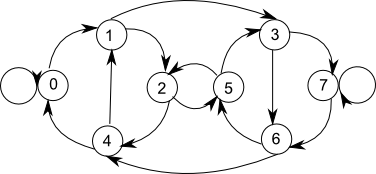
\includegraphics[width=0.5\textwidth]{img_2_1.png} 
\caption{Grafo dirigido}
\end{figure}


Si $M_{R_i} \quad i=1,2$ es una representación en matriz booleana de la relación $R_i$, entonces tenemos:

$$M_{R_1\cup R_2}=M_{R_1}\lor M_{R_2}\quad ; \quad
M_{R_1\cap R_2}=M_{R_1}\land M_{R_2}$$

\section{Posets}
Un conjunto S junto con una relación de orden parcial R se denomina un conjunto parcialmente ordenado o Poset y se le denota por $(S,R)$. En el caso de los Posets se usa la notación $aRb$ para indicar que $(a,b)\in R$.\\
\textbf{Ejemplo: } Si $\backslash$ denota la relación de divisibilidad entre enteros, entonces el par $(\mathds{N},\backslash)$ es un poset.\\
\textbf{Ejemplo: }\\
$\begin{array}{rl}7\in \mathds{N}, (7,7)\in \backslash \quad & reflexiva.\\
(6,2)\in \backslash \land 6\not=2 \; pero\; (2,6)\not\in \backslash \quad & antisimetrica.\\
(16,8)\in R \land (8,2)\in R \rightarrow (16,2)\in R \quad & transitiva.\end{array}$\\
 
Si A es cualquier conjunto, entonces $(2^A,\subseteq)$ es también un poset. Los posets pueden ser representados gráficamente mediante los diagramas Hasse. Estos están basados en el hecho que si $aRb \land bRc$ en un Poset (S,R) entonces $aRc$.\\
Sea (S,R) un poset. Denotamos $R_H \subseteq R$ la relación definida como sigue: $aR_H b$ si y solo si aRb y no hay $a\not=c\not=b$ tal que aRc y cRb.\\
En otras palabras $R_H$ es el conjunto mas pequeño con $R_H^*=R$.\\
\textbf{Ejemplo: }Sea $S=\lbrace 0,1,3\rbrace \; y \; R =\subseteq$, graficaremos el Poset $(2^S, \subseteq)$\\
$2^S=\lbrace \phi,\lbrace 0\rbrace,\lbrace 1\rbrace,\lbrace 2\rbrace,\lbrace 0,1\rbrace,\lbrace 0,2\rbrace,\lbrace 1,2\rbrace, S\rbrace$

\begin{figure}
\centering 
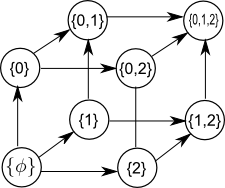
\includegraphics[width=0.35\textwidth]{img_2_2.png}
\caption{Gráfico del Poset}
\end{figure}

\section{Funciones}
El conjunto $f\subset A\times B$ es una función si:
\begin{itemize}
\item $Dom(f)=A$
\item Si $(x,y),(x,z)\in f \; entonces\; y=z$
\end{itemize}
Esto significa que para todo elemento x en A, existe un único y tal que $(x,y)\in f$.\\
\textbf{Notación: } $f:A\rightarrow B\\
					y=f(x)\quad(x,y)\in f$
					
A una función de éstas características la denominaremos función total.\\

\textbf{Teorema: }Sean las funciones $f:A\rightarrow B\; y\; g:A\rightarrow B$ Entonces $f=g$ si $f(x)=g(x) \forall x\in A$.

\subsection{Función Parcial}
Una relación $f\subseteq A\times B$ se denomina función parcial si:
\begin{itemize}
\item $Dom(f)\subseteq A$
\item Si $(x,y),(x,z)\in f\; entonces\; y=z$
\end{itemize}

\subsection{Imagen}
Sea $f:A\rightarrow B$ una función. Si $X\subseteq A$ se dice la imagen de X bajo f a : $f(x)=\lbrace y\in B/ y=f(x) ; para\; x\in X\rbrace$

\subsection{Imagen Inversa}
Sea $Y\subseteq B$, la imagen inversa de Y bajo f es: $f^{-1}(Y)=\lbrace x\in A / f(x)=y$ para algún $y\in Y\rbrace$

\textbf{Definición: } Sea $f:A\rightarrow B$ una función. Su rango es: $\lbrace f(x)/x\in A\rbrace$ que es un subconjunto del codominio B.

\subsection{Tipos Especiales de Funciones}
Sea $f:A\rightarrow B$ una función.
\begin{enumerate}
\item \textbf{Función Inyectiva: }f es inyectiva ó 1 a 1 si cumple:\\
	Para cualquier $(x,z)\in f \land (y,z)\in f\Rightarrow x=y$ o equivalente: si $f(x)=f(y) \Rightarrow x=y$
\item \textbf{Función Sobreyectiva: }f es sobreyectiva si su rango es todo el conjunto B o equivalente. $\forall y\in B, \exists x\in A / y=f(x)$
\item \textbf{Función Biyectiva: }Si f es a la vez inyectiva y sobreyectiva se dirá biyectiva. Cuando f es una biyección, $f^{-1}:B\rightarrow A$ es una función. La función inversa $f^{-1}:B\rightarrow A$ satisface:\\
$f^{-1}(f(x))=x \land f(f(f^{-1}(x))=y$
\end{enumerate}

\textbf{Ejemplo: }Para las siguientes funciones indique si son inyectivas y/o sobreyectivas.
\begin{enumerate}
\item $f:\mathds{N}\rightarrow \mathds{N} / f(n)=n$
\item $g:\mathds{N}\rightarrow \mathds{Z} / g(n)=n+1$
\item $h:\mathds{R}\rightarrow \mathds{R} / h(x)=x^2$
\end{enumerate}

\textbf{Solución: }Analizando cada uno de los casos.
\begin{itemize}
\item f es inyectiva, f es sobreyectiva.
\item g es inyectiva pero no sobreyectiva.
\item Si $h(x)=h(y)\\
			x^2=y^2\\
			\rightarrow x=y \lor x=-y$, entonces h no es inyectiva.
\item Si $y=-8, \not\exists x\in \mathds{R} / h(x)=y$ , entonces h no es sobreyectiva.
\end{itemize}

\section{Composición de Funciones}
Sean $f:A\rightarrow B \land g:C\rightarrow D$ definimos $g\circ f: A\rightarrow D$\\



$g\circ f(x)= \left \{  \begin{array}{rp{1cm}l} g(f(x)) & &x\in Dom\, f \land f(x)\in Dom\, g
				\\	indefinido & &\mbox{para otros casos}\end{array}\right.$\\

En general $f\circ g\not=g\circ f$\\

\textbf{Ejemplo: }Sean: $$\begin{array}{l} f:\mathds{Z}\rightarrow \mathds{N}/f(n)=|n|+1 \\
										g:\mathds{N}\rightarrow\mathds{Z}/g(n)=1-n\end{array}$$
Halle $f\circ g, g\circ f$.
\chapter{Operaciones Binarias}

Sea A un conjunto, una operación binaria en A es una función $f:A\times A \rightarrow A$.
\begin{itemize}
\item $Dom(f)=A\times A$
\item Solo un elemento de A se asigna a cada par (a,b)
\end{itemize}

\textbf{Convención: }Usaremos * en vez de f. $a*b \mbox{ en vez de f(a,b)}$.\\
\textbf{Ejemplo: }
\begin{enumerate}
\item Si $A=\mathds{Z}$ Definiendo a*b = a+b.\\
		* es na operación binaria.
\item Sea $A=\mathds{R}$ y definimos $a*b=a/b$\\
		* no es una operación binaria pues para (a,0) no está definida a*0.
\item Sea $A=\mathds{Z}^+$ y definimos $a*b=a-b$\\
		* no es una operación binaria (ejem: 3*7 = -4, -4 no pertenece a A)
\item Sea $A=\mathds{Z}$ y sea $a*b=max(a,b)$\\
		* es una operación binaria.
\item Dado un conjunto S y su respectivo P(S). Si V y W son subconjuntos de S, definimos $V*W=V\cup W$\\
		\textbf{Ejemplo: }$S=\lbrace 1,3,5\rbrace$\\
		$P(S)=\lbrace \phi,\lbrace 1\rbrace,\lbrace 3\rbrace,\lbrace 5\rbrace,\lbrace 1,3\rbrace,\lbrace 1,5\rbrace,\lbrace 3,5\rbrace, S\rbrace$\\
		$\lbrace 3\rbrace * \lbrace 1,5\rbrace =\lbrace 1,3,5\rbrace$\\
		* es una operación binaria.
\end{enumerate}

Para un conjunto finito $A=\lbrace a_1,a_2,...,a_n\rbrace$ podemos definir una operación binaria mediante la tabla.

\begin{center}
\begin{tabular}{c|ccc}
* & $a_1 \quad a_2$&$...\; a_j\; ...$&$a_n$\\ \hline
$a_1$ & &   $\vdots$&\\
$a_2$ &    &$\vdots$&\\
$\vdots$ &   &$\vdots$&\\
$a_i$ & $\cdots \cdots$& $a_i*a_j$&\\
$a_n$ & & &
\end{tabular}
\end{center}

\textbf{Ejemplo: }Sea $A=\lbrace 0,1\rbrace$ podemos representar las operaciones binarias $\lor,\land$ mediante.
%foto2
\begin{center}
\begin{tabular}{cp{2cm}c}
\begin{tabular}{c|cc}
$\lor$ & 0 & 1\\ \hline
0	&	0	&	1\\
1	&	1	&	1\\
\end{tabular}
& &
\begin{tabular}{c|cc}
$\land$ & 0 & 1\\ \hline
0	&	0	&	0\\
1	&	0	&	1\\
\end{tabular}
\end{tabular}
\end{center}

\section{Propiedades de las Operaciones Binarias}

\textbf{P1: }Una operación binaria * es conmutativa si $a*b=b*a \quad \forall a,b \in A$\\
\textbf{Ejemplo: }De los ejemplos anteriores.
\begin{enumerate}
\item $A=\mathds{Z}\quad *=+$\\
		* es conmutativa: a+b = b+a.
\item $A=\mathds{Z}^+ \quad \quad *=-$\\
		* no es conmutativa: $\begin{array}{rll}3*5&\not=&5*3 \\ -2&\not=&2\end{array}$
\item Sea $A=\lbrace a,b,c,d\rbrace$ Cuál de las siguientes representaciones es conmutativa?
\begin{center}
\begin{enumerate*}
\item
\begin{tabular}{c|cccc}
*	&a	&b	&c	&d \\ \hline
a	&a	&c	&b	&d \\
b	&b	&c	&b	&a \\
c	&c	&d	&b	&c \\
d	&a	&a	&b	&b \\
\end{tabular}
\item
\begin{tabular}{c|cccc}
*&a&b&c&d\\ \hline
a&a&c&b&d\\
b&c&d&b&a\\
c&b&b&a&c\\
d&d&a&c&b\\
\end{tabular}
\end{enumerate*}
\end{center}

Entonces:
\begin{itemize}
\item $\left.\begin{matrix} a*b & =c \\ b*a & =b \end{matrix}\right\}$ * no es conmutativa.

\item $a*b=c=b*a\\ c*d=c=d*c \\ d*a=d=a*d$\\ Si la matriz de resultados M verifica que $M=M^T$, la operación es conmutativa. * es conmutativa.

\end{itemize}
\end{enumerate}

\textbf{P2 :}Una operación binaria  * es asociativa si:
$(a*b)*c=a*(b*c)\quad \forall a,b,c \in A$

\textbf{Ejemplo: }
\begin{enumerate}
\item Sea $A=\mathds{Z}$ y * = +\\
		* es asociativa
\item Si $A=\mathds{Z}$ y * = -\\
		* no es asociativa\\
		$\begin{array}{rll}		
		(3*5)*2&\not=& 3*(5*2)\\
		-2*2 &\not=& 3*3\\
		-4 &\not=& 0\end{array}$
\end{enumerate}

\section{Semigrupo}

Un semigrupo es un conjunto no vacío S, junto a una operación binaria asociativa * definida sobre S.\\
\textbf{Notación: }Denotamos al semigrupo por (S,*). Adicionalmente si * es conmutativa se dirá semigrupo conmutativo.\\
\textbf{Ejemplo: }
\begin{enumerate}
\item $(\mathds{Z},+)$ es semigrupo conmutativo.
\item $(\mathds{Z},-)$ no es semigrupo.
\item Para un conjunto S, $(P(S), \cup)$ es semigrupo conmutativa.
\item Sea S un conjunto no vacío, denotamos $S^S$ como el conjunto de todas las funciones $f:S\rightarrow S$\\
		Sean $f,g\in S^S \, definimos: \; f*g=f\circ g$\\
		$(S^S,*)$ es un semigrupo. Sin embargo no es conmutativa, porque $f\circ g\not= g\circ f$
\end{enumerate}

\textbf{Definición } A un elemento ''e'' en el semigrupo (S,*) se le llama identidad si: $$a*e=a=e*a\quad\quad \forall a\in S$$
\textbf{Ejemplo: }
\begin{enumerate}
\item Si $(\mathds{Z},+)$ se tiene el elemento identidad, es e = 0.
\item En el semigrupo $(\mathds{Z}^+,-)$ no hay elemento identidad.
\end{enumerate}
		
\textbf{Teorema: }S un semigrupo $(S,*)$ tiene elemento identidad, éste debe ser único.\\
\textbf{Prueba: } Supongamos que $e_1\; y\; e_2$ son elementos identidad. Como $e_1$ es identidad: $e_2 * e_1 = e_2 = e_1*e_2$\\
$e_2$ es identidad: $e_1*e_2=e_1=e_2*e_1$\\
$e_2=e_1*e_2=e_1$, luego sólo hay un elemento identidad.

\textbf{Definición: } Un semigrupo es un monoide si tiene elemento identidad.\\
\textbf{Ejemplo: }
\begin{enumerate}
\item El semigrupo $(P(S),\cup)$ donde S es un conjunto no vacío, tiene elemento identidad $e=\phi$, pues $\phi \cup V=V$. El semigrupo es un monoide.
\item En el semigrupo $(S^S,\circ)$ se tiene elemento identidad $e=id_S$\\
		$id_S \circ f = f=f\circ id_S \quad\quad \forall f\in S^S$\\
		$(S^S,\circ)$ es un monoide.
\end{enumerate}

\textbf{Definición: }Sea (S,*) un semigrupo y sea $T\subset S$. Si T es cerrado bajo la operación * [ si $a,b\in T$ entonces $a*b\in T$] entonces $(T,*)$ es un subsemigrupo de $(S,*)$.

\textbf{Definición: }Sea (S,*) un semigrupo y sea $\phi\not= T\subset S$. Si T es cerrado bajo * y $e\in T$, entonces a (T,*) se le llama submonoide de (S,*).

\section{Isomorfismos}

Sean (S,*),(T,*') dos semigrupos. A la función $f:S\rightarrow T$ , se le llama isomorfismo de (S,*) en (T,*') si f es inyectiva, sobreyectiva y además  $f(a*b)=f(a)*' f(b) \quad\quad \forall a,b\in S$.\\
\textbf{Notación: }Si los semigrupos (S,*) y (T,*') son isomorfos se le denota por $S\simeq T$.\\

\textbf{Método: }Para demostrar que $S\simeq T$, se seguirá el procedimiento:
\begin{enumerate}
\item Defínase una función $f:S\rightarrow T$
\item Verifique que f sea inyectiva
\item Verifique que f sea sobreyectiva
\item Demuestre que $f(a*b)=f(a)*' f(b)$
\end{enumerate}

\textbf{Ejemplo: }Sea T el conjunto de los pares. Demuéstrese que los semigrupos $(\mathds{Z},+)$ y $(T,+)$ son isomorfos.\\
\textbf{Solución: } 
\begin{enumerate}
\item Definimos la función $f:S\rightarrow T$.  $f(x)=2x\quad \quad x\in \mathds{Z}$

\item Sean $x_1,x_2$:
\begin{center}
$f(x_1)=f(x_2)$ \\$2x_1=2x_2$ \\ $x_1=x_2$\\
f es inyectiva.
\end{center}
\item Sea $b\in T$ cualquiera, luego $b=2a \quad a\in \mathds{Z}$\\
$f(a)=f(\frac{b}{2})=\not2.\frac{b}{\not2}=b$\\
Luego f es sobreyectiva.

\item P.P que: $f(a*b)=f(a)*' f(b) \\
				f(a*b)=2(a*b)=2a+2b=f(a)+f(b)\\
				f(a*b)=f(a)*'f(b)$\\
				Luego $\mathds{Z}\simeq T$.						
\end{enumerate}

Sean (S,*),(T,*') dos semigrupos finitos y sus operaciones las expresamos mediante tablas. Entonces $S\simeq T$ si es posible reordenar y etiquetar los elementos de S para que su tabla sea idéntica a la tabla de T.\\
\textbf{Ejemplo: }Sean $S=\lbrace a,b,c\rbrace$ y $T=\lbrace x,y,z\rbrace$ con tablas respectivas.

\begin{center}
\begin{tabular}{cp{2cm} c}
\begin{tabular}{c|c}
* & a b c\\ \hline
a & a b c\\
b & b c a\\
c & c a b
\end{tabular}
& &
\begin{tabular}{c|c}
*' & x y z\\ \hline
x & z x y\\
y & x y z\\
z & y z x
\end{tabular}
\end{tabular}



\end{center}

Sea:
\begin{center}
$f(a)=y $\\ $f(b)=x$\\ $f(c)=z$
\end{center}

\begin{center}
\begin{tabular}{c c c}
\begin{tabular}{c|c} 
  & y x z\\ \hline
y & y x z\\
x & x z y\\
z & z y x
\end{tabular}%
& $\rightarrow$ &
\begin{tabular}{c|c}
  & x y z\\ \hline
x & z x y\\
y & x y z\\
z & y z x
\end{tabular}
\end{tabular}

\end{center}

Luego $S\simeq T$.\\

\textbf{Teorema: }Sean los semigrupos (S,*) y (T,*') monoides y con identidades $e$ y $e'$. Sea f un isomorfismo, entonces $e'=f(e)$.\\
\textbf{Demostración: }Sea $b\in T$. Al ser f un isomorfismo, es sobreyectiva, existe $a\in S/ f(a)=b$.\\
Como $e$ es identidad:
\begin{itemize}
\item 	
$\begin{array}{lll}
a	& =	& a*e\\
f(a)& =	& f(a*e)\\
b 	& =	& f(a)*'f(e)\\
b	& = & b*'f(e)
\end{array}$		
		
\item   
$\begin{array}{lll}
a	& =&e*a\\
f(a)& =&f(e*a)\\
b	& =&f(e)*'f(a)\\
b	& =&f(e)*'b \end{array}$
\end{itemize}

Del 1er y 2do item, $b*'f(e)=b=f(e)*'b$, luego $f(e)$ es identidad en T, $\therefore e'=f(e)$.\\

\textbf{Definición: }Sean (S,*) y (T,*') dos semigrupos. A una función $f:S\rightarrow T$. Se le llama un homomorfismo si:
$$f(a*b)=f(a)*'f(b)\quad\quad \forall a,b\in S$$

\chapter{Grupo}

Un grupo $(G,*)$ es un monoide tal que satisface las siguientes propiedades.
\begin{description}
\item [P1 Propiedad asociativa: ]$(a*b)*c= a*(b*c)\quad \forall a,b,c \in G$.
\item [P2 Existencia de una identidad: ]Existe un elemento único $\in$ G tal que :
	$a*e=a=e*a$ $a\in G$.
\item [P3 Existencia del elemento inverso: ]$\forall$ G, existe el elemento inverso denotado por  $a' \in G$ tal que:
$a*a'=e=a'*a$.
\end{description}

En un grupo $(G,*)$, * operación binaria, G deberá ser cerrada bajo *, es decir.
$a*b \in G \quad \forall a,b \in G$.

\textbf{Definición: }Si $(G,*)$ es conmutativo, es decir: $a*b=b*a$, se le llamará \textbf{Abeliana}.\\

\textbf{Ejemplo: }$(\mathds{Z},+)$
\begin{itemize}
\item P1 se cumple.
\item P2 e=0.
\item P3 $y\in \mathds{Z} \quad \exists y\in \mathds{Z} \quad \quad y*y'=e$
\end{itemize}

\textbf{Ejemplo: }$(\mathds{Z}^+,\cdot)$
\begin{itemize}
\item P1 si.
\item P2 si.
\item P3 no.
\end{itemize}

\textbf{Ejemplo: }$(\mathds{R}-\lbrace 0 \rbrace,\cdot)$
\begin{itemize}
\item P1 si.
\item P2 e=1.
\item P3 si.
\end{itemize}

\textbf{Ejemplo: }Sea G el conjunto de los reales sin el ''cero'' y sea $a*b=\frac{ab}{2}; a,b\in G$ Pruebe que $(G,*)$ es Grupo.\\
* es una operación binaria.
\begin{itemize}
\item $Dom=G\times G \; ; \quad *G\times G \rightarrow G$.
\item $a*b= \frac{ab}{2}$ es único $\forall a,b\in G$.
\end{itemize}

\begin{enumerate}
\item Veamos que $(G,*)$ es asociativa.\\
$(a*b)*c=(\frac{ab}{2})*c=\frac{abc}{4}$\\
$a*(b*c)=a*({bc\over2})={abc\over4}$\\
$(a*b)*c=a*(b*c)$

\item Afirmamos que $e=2$ es la identidad.\\
$a*e= \frac{a(2)}{2} = a$\\
$e*a=\frac{2(a)}{2}=a$

\item Afirmamos que $a'={4\over a} \in G$ es la inversa de a.\\
$a*a'=\frac{a({4\over a})}{2} = 2 = e$\\
$a'*a=\frac{({4\over a})(a)}{2}=2=e$\\
$\therefore$ G es un grupo.
\end{enumerate}

\textbf{Teorema 1: }Sea G n grupo . Cada elemento $a\in G$ tiene un inverso único en G.\\

\textbf{Teorema 2: }Sea G un grupo y sean a,b,c elementos en G. Entonces.
\begin{itemize}
\item $a*b=a*c \Rightarrow b=c$ Propiedad cancelativa izquierda.
\item $b*a=c*a \Rightarrow b=c$ Propiedad cancelativa derecha.
\end{itemize}

\textbf{Teorema 3: }Sea $(G,*)$ un grupo y $a,b\in G$. Entonces.
\begin{itemize}
\item $(a')'=a$
\item $(a*b)'=b'*a'$
\end{itemize}

Si G es un conjunto finito, su operación binaria * se puede obtener mediante una tabla.\\
Sea $G=\lbrace a_1,a_2,...a_n\rbrace$. La tabla de multiplicación bajo * cumple:
\begin{itemize}
\item La fila etiquetada por $e$ deberá contener a:  $a_1, a_2, \cdots a_n$
\item La columna etiquetada por $e$ debe contener a:  $\begin{matrix}a_1\\a_2\\a_3\\ \vdots \\ a_n\end{matrix}$

\item Cada elemento ''b'' en el grupo deberá aparecer exactamente una vez en cada fila y en cada columna.
\end{itemize}

\textbf{Definición: }Sea $(G,*)$ un grupo que tiene un número finito de elementos.
\begin{itemize}
\item Se dice que G es finito.
\item El orden de G es el número de elementos y se denota por $|G|$.
\end{itemize}


\textbf{Ejemplo: }
\begin{itemize}
\item Si G es unitario, $G=\lbrace e\rbrace$ , $e*e=e$.
\item Si $|G|=2, G=\lbrace e,a\rbrace$.Su tabla es:

\begin{tabular}{c|cc}
 &e&a\\ \hline
e&e&a\\
a&a&e
\end{tabular}
$\begin{matrix}
a'=a \\
e'=e
\end{matrix}$
\item Si $|G|=3, G=\lbrace e,a,b\rbrace$. Su tabla es:\\
\begin{tabular}{c|ccc}
 &e&a&b\\ \hline
e&e&a&b\\
a&a&b&e\\
b&b&e&a
\end{tabular}

$\begin{matrix} a*b=e \quad & a'=b\\
b*a=e \quad & b'=a\\
e*e=e \quad & e'=e\end{matrix}$
\end{itemize}

\textbf{Ejemplo: }Sea $B=\lbrace 0,1\rbrace$ y $*=+$
\begin{center}
\begin{tabular}{c|cc}
+&0&1\\ \hline
0&0&1\\
1&1&0
\end{tabular}

$\begin{matrix}
0*0=0 \quad 0'=0\\
1*1=0 \quad 1'=1
\end{matrix}$
\end{center}

\section{Cadenas}

Un tipo de problema a revisar es el de decisión. Un problema de decidibilidad es una función que produce como resultado uno de dos valores: ''si'' o ''no''.\\

\textbf{Definición: }Un símbolo es un objeto indivisible. Utilizaremos como símbolos las letras iniciales del alfabeto y los dígitos.

\textbf{Definición: }Un alfabeto es un conjunto finito o infinito de símbolos.\\
\textbf{Notación: }$\sum , V,\Gamma$\\

\textbf{Ejemplo: }
\begin{enumerate}
\item Alfabeto Binario $\Sigma = \lbrace 0,1\rbrace$
\item Alfabeto de letras mayúsculas $\Sigma =\lbrace A,B,C,...,Z\rbrace$
\end{enumerate}

\textbf{Definición: }Una cadena ó palabra es una secuencia finita de símbolos, tomados a partir de un alfabeto.\\
\textbf{Notación: } $W (x,y,...)$.\\
Sea $W=a_1,a_2,...a_k$ con $a_i \in \Sigma$, $i=1,...k$\\
Longitud:\\
$|W|=k \Leftrightarrow W=a_1...a_k$\\
Sea $\Sigma=\lbrace 0,1 \rbrace$ y $W=001101 \Rightarrow |W|=6$

\section{Cadena Vacía}

Es la cadena de longitud ''cero''.\\
\textbf{Notación: }$\varepsilon, \lambda$.
\textbf{Notación: }Denotamos por $W_k$ al conjunto de todas las cadenas de longitud $k$ sobre un alfabeto $\Sigma$.\\

$W_k=\lbrace W/|W|=k$ y $W=a_1...a_k; a_i\in \Sigma \rbrace$\\

$W_0=\lbrace \varepsilon \rbrace $ y lo denotamos por $\varepsilon$ \\ %negrita
Al conjunto de todas las cadenas finitas posibles.

Sobre $\Sigma$, lo denotamos por $W= \bigcup_{k=0}^\infty W_k$

\section{Operación con Cadenas}
\subsection{Concatenación}
El producto de cadenas es una operación binaria en W.\\
$m:W\times W \rightarrow W$\\
Si $x=a_1,...a_i; y=b_1...b_j$ entonces $m(x,y)=a_1...a_i,b_1...b_j$. Denotamos $m(x,y)$ por $x.y$ ó simplemente $xy$.\\

\textbf{Definición: }Sea $W=xz$. Entonces:\\
''x'' es un prefijo de W, es un prefijo propio si $z\not= \varepsilon$\\
''z'' es un sufijo de W, es un sufijo propio si $x\not=\varepsilon$

\subsection{Propiedades de la Concatenación}
Sea $W=xyz$
\begin{enumerate}
\item \textbf{Cerradura: }$\forall x, y\in W \quad xy\in W$
\item \textbf{Asociatividad: }$(x.y).z=x.(y.z) \quad x,y,z\in W$
\item \textbf{Identidad: }$w.\varepsilon = w = \varepsilon .w \quad \forall w\in W$
\item \textbf{Longitud: }Para $wx \Rightarrow \quad |wx|=|w|+|x| \quad w,x \in W$
\end{enumerate}
La concatenación no necesariamente es conmutativa. $wx\not=xw$ En general.\\
\textbf{Notación: }$w^k=\underbrace{ww...w}_{k\; veces}$

Si $w=a_1...a_k$ entonces $w^R=a_k...a_1$

\section{Lenguajes}
Un lenguaje L es un conjunto de cadenas definidas sobre $\Sigma$.\\
$L\subset W$\\

\textbf{Ejemplo: }
\begin{enumerate}
\item Sea $\Sigma = \lbrace a_0,a_1\rbrace$. Entonces:\\
	$L=\lbrace a_0 a_1...a_{i_k} / a_{i_j} \in \Sigma \rbrace$ es un lenguaje.

\item Sea $\Sigma = \lbrace a\rbrace$\\
	$L=\lbrace a^k / k>0 \rbrace$ es el lenguaje de todas las cadenas de ''a'' de longitud finita.

\item Sea $\Sigma=\lbrace 0,1\rbrace$\\
	$L=\lbrace ww^R/w=a_1...a_k \quad a_i \in \Sigma\rbrace$ L es el lenguaje de los palíndromos formados con ceros y unos.
\end{enumerate}

\section{Operaciones con Lenguajes}
Sean $L_1, L_2$ dos lenguajes. Definimos las siguientes operaciones:\\

$\begin{array}{rl}L_1\cup L_2 &=\lbrace w/w \in L_1 \lor w \in L_2\rbrace\\
L_1\cap L_2 &= \lbrace w/w\in L_1 \land w\in L_2\rbrace\\
I &=\lbrace w/w \not \in L \land w=a_1...a_k; \quad a_i\in \Sigma\rbrace\\
L_1.L_2 &=\lbrace vw/v\in L_1 \land w\in L_2\rbrace
\end{array}$\\

\textbf{Propiedad: }La cardinalidad de la concatenación de dos lenguajes es menor o igual que el producto de las cardinalidades de cada uno de ellos.\\

\textbf{Ejemplo: }Sean $L_1=\lbrace a,ab\rbrace \quad L_2=\lbrace c,bc\rbrace$ sobre $\Sigma =\lbrace a,b,c\rbrace$\\
$\begin{array}{rl}L_1 L_2 &=\lbrace ac,abc,...,abbc\rbrace\\
|L_1 L_2| &\leq |L_1||L_2|\\
3 &\leq 2\times 2
\end{array}$

\textbf{Propiedad (Identidad): }El conjunto $L_\varepsilon =\lbrace \varepsilon \rbrace$ es la identidad en la concatenación de lenguajes.\\
$L.L_\varepsilon =\lbrace w.x/w\in L,x\in L_\varepsilon \rbrace = \lbrace w/w\in L\rbrace$ como $w.\varepsilon = w= \varepsilon . w$\\
$L_\varepsilon .L= L.L_\varepsilon = L$\\ %lenguaje identidad

\textbf{Elemento Nulo: }Es el conjunto vacío $\phi$.\\

\textbf{Propiedad Asociativa } $(L_1 L_2)L_3=L_1(L_2 L_3)$\\

\textbf{Propiedad Distributiva }$L_1(L_2\cup L_3)=L_1 L_2 \cup L_1 L_3$\\

¿Es la concatenación de lenguajes distributiva respecto a la intersección?\\

\textbf{Definición: }Sea $\Sigma$ un alfabeto y $L\subseteq W$ un lenguaje sobre $\Sigma$. Definimos las siguientes potencias de L:\\

$\begin{array}{rl}
L^0 &= \lbrace \varepsilon \rbrace\\
L^1 &=L \\
L^k &=L^{k-1}.L
\end{array}$\\

\textbf{Definición: }La cerradura del lenguaje L es $L^* =\bigcup_{k=0}^\infty L^k$. Al operador * se le llama ''Estrella de Kleene'' o ''Cerradura de Kleene''.\\

\textbf{Ejemplo: }Sea $\Sigma=\lbrace a,b,c\rbrace$ y $L=\lbrace a,ab,ac\rbrace$. Halle: $L^2, L^3$.\\

$L^2=L.L=\lbrace aa,aab,aac,aba,abab,abac,aca,acab,acac \rbrace$\\
$L^3=L^2 .L=\lbrace aaa,aaab,aaac,aaba,aabab,aabac,\\ aaca,aacab,aacac,...acaca,acacab,acacac \rbrace$

\textbf{Ejemplo: }Sea $L=\lbrace a\rbrace \quad \Sigma =\lbrace a \rbrace$\\
$L^* =\lbrace \varepsilon, a,aa,aaa,... \rbrace$\\

\textbf{Ejemplo: }Sea $L=\lbrace 0,1,00,01 \rbrace \quad \Sigma = \lbrace 0,1\rbrace$\\
$L^* = \lbrace \varepsilon , 0,1,00,01,00,01,000,001,... \rbrace$\\

\textbf{Ejemplo: }Sea L un lenguaje. $L^R=\lbrace w^R/ w\in L\rbrace$\\
Sea ahora $L=\lbrace ww^R/w=a_1...a_k ; a_i \in \Sigma \rbrace$\\
a este lenguaje se le conoce como ''Lenguaje espejeado''. %diferencia entre espejeado y palindromo es que este ultimo es mas general obs

% ver una forma simplificada de algunos lenguajes, pendiente.
\chapter{Lenguajes Formales}

En oposición al lenguaje natural, un lenguaje formal es tal que:
\begin{enumerate}
\item Tiene una sintaxis bien definida. De tal modo que dada una sentencia, es posible saber si pertenece o no al lenguaje.
\item Tiene una semántica precisa. No es posible encontrar sentencias ambiguas o sin significado.
\end{enumerate}
\textbf{Ejemplo: }C, Java, HTML.

\section{Lenguajes Regulares}

Son un tipo de Lenguaje Formal. Reciben este nombre porque sus palabras contienen regularidades o repeticiones de los mismos componentes.

\textbf{Ejemplo: }
\begin{itemize}
\item $L_1=\{cd,cdcd,cdcdcd,...\}$

Las cadenas contienen las subcadenas un número dado de veces.
\item $L_2=\{ abc,cc,abab,abccc,ababc,...\}$

La regularidad consiste encadenas que empiezan con repeticiones de ''ab'' seguidas de repeticiones de c.
\end{itemize}

Se considerará a los lenguajes finitos también regulares.

$L_3=\{ hoy, es, sabado \}$ $L_3$ es regular.

\section{Aplicación}

Se pueden utilizar para especificar la generación de analizadores léxicos.
\subsection{Analizadores Léxicos}

Es un programa que recibe como entrada el código fuente de otro programa y produce como salida Lexemas.

Las palabras están compuestas por lexemas y morfemas.

\subsubsection{Lexema}
Es la raíz o parte de la palabra que no varía.

\textbf{Ejemplo: }\textbf{deport}-e, \textbf{deport}-ivo, \textbf{deport}-ista.
\subsubsection{Morfema}
Es la parte que se le añade al lexema para completar su significado y así generar nuevas palabras.

\textbf{Ejemplo: }moder-\textbf{o}, modern-\textbf{as}, modern-\textbf{ísimo}.

\subsection{Definición Recursiva}

Sea un alfabeto $\Sigma$, Un lenguaje $L\subseteq \Sigma^*$ regular se define recursivamente como sigue.
\begin{itemize}
\item $\phi$, el lenguaje vacío, es un lenguaje regular.
\item $\{ \varepsilon \}$ es un lenguaje regular.
\item $\{ a \}$ es un lenguaje regular $\forall a\in \Sigma$.
\item Si $L_1$ y $L_2$ son lenguaje regulares, entonces $L_1 \cup L_2, L_1 \cdot L_2 ,L_1^*$ son lenguajes regulares.
\item Ningún otro lenguaje sobre $\Sigma$ (definida en las 4 anteriores) es un lenguaje regular.
\end{itemize}

\textbf{Ejemplo: }Sea $\Sigma =\{ a,b \}$. Encuentre 6 lenguajes regulares.

$\begin{array}{rl}
L_1 &=\phi \\
L_2 &=\{a\} \quad L_4\{b\}\\
L_5 &=\{a,b\} \quad L_6=\{ ab\} \quad L_7=\{ a,ab,b\}
\end{array}$

\textbf{Ejemplo: }Dado $\Sigma = \{ a,b\}$. Describa 3 L.R. infinitas y representarlos de forma abreviada.

$L_1=\{ w\in \Sigma^* / w$ empieza con $b\}$ $=\{b\}\Sigma^*$

$L_2=\{ w\in \Sigma^* / w$ contiene exactamente una $a\}$ $=\{b\}^* \cdot\{a\} \cdot\{ b\}^*$

$L_3=\{ w\in \Sigma^* / w \mbox{ contiene a la subcadena } ba\}$ \\
$\begin{array}{p{0.65cm}l}
   &=\{ ba,aaba,bbabba,abbaaab,...\} \\
   &=\Sigma^* \{ ba\}\Sigma^*
\end{array}$

$L_4=\{ w\in\Sigma^* / w$ contiene exactamente dos símbolos $b\}$ $=\{a\}^* \{b\}\{a\}^* \{b\}\{a\}^*$

$L_5=\{a^k /k \geq 0, a\in\Sigma \}$


\section{Características}
Un L.R tiene estas características.
\begin{enumerate}
\item Puede ser escrito mediante una ''Expresión Regular''.
\item Puede ser reconocido mediante un ''Autómata Finito''.
\item Puede ser generado mediante una ''Gramática Regular''.
\end{enumerate}

\section{Expresiones Regulares (ER)}
Una ER es una secuencia de caracteres que forma un patrón de búsqueda. Se usa para especificar un conjunto de cadenas requeridas para un propósito particular.

\textbf{Aplicaciones: }
\begin{itemize}
\item Búsqueda de patrones de cadenas de caracteres.
\item Operaciones de sustitución.
\end{itemize}

\textbf{Ejemplo: }Dadas las cadenas Handel, H\"andel, Haendel. Describa el patrón que los especifique.

H$\{a|\ddot{a}|ae\}$ndel

\subsection{Definición Recursiva}
Dado un alfabeto $\Sigma$, una ER se define recursivamente como sigue:
\begin{itemize}
\item El símbolo $\phi$ es una ER.
\item $\varepsilon$ es una ER.
\item $a\in\Sigma$, es una ER.
\item Si p y q son ER, entonces p.q, p$\cup$q, p* son ER.
\end{itemize}

Se cumple que toda ER sobre $\Sigma$ describe a un LR sobre $\Sigma$.

\textbf{Abreviatura: }

Para los lenguajes siguientes, a continuación se dan las abreviaturas correspondientes.

$\begin{array}{cc}
 & \mbox{Exp. Regulares} \\
\{v\}\cup \{w\} & v+w\\
\{v.w\} & vw\\
\{w\}^* & w^*\\
\{w\}^+ & w^+\\
\end{array}$

\subsection{Nivel de Prioridad}

$\begin{array}{cc}

\mbox{Operador} & \mbox{Prioridad} \\
* & 1 \\
\cdot & 2 \\
+ & 3
\end{array}$

\textbf{Ejemplo: }Reducir la expresión. $E=( \{ a\}^*\{b\} )\cup \{c\}$.

Queda: $a^*b+c$, mediante las ER.

\textbf{Definición: }Dada una expresión regular $\alpha$, denotado por $L(\alpha)$ como:

\begin{itemize}
\item $L(\phi)=\phi$
\item $L(\varepsilon)=\{\varepsilon\}=L_\varepsilon$
\item $L(a)=\{a\}$, donde $a\in\Sigma$
\item $L(\alpha \cdot \beta)= L(\alpha)\cdot L(\beta)$, donde $\alpha, \beta$ son ER.
\item $L(\alpha +\beta)=L(\alpha)\cup L(\beta)$, donde $\alpha, \beta$ son ER.
\item $L(\alpha^*)=(L(\alpha))^*$
\end{itemize}

\section{Equivalencia de ER}

\textbf{Definición: }Dadas las ER $\alpha,\beta$ definidas sobre $\Sigma$, diremos que son equivalentes si ambas generan el mismo lenguaje.

$L(\alpha)=L(\beta)$

\textbf{Notación: }Si $\alpha$ y $\beta$ son equivalentes se denotará $\alpha =\beta$.
\section{Propiedades de las ER}

Sea $\Sigma$ un alfabeto $\alpha,\beta$ y $\gamma$ ER. Se cumple:
\begin{enumerate}
\item $\alpha+\beta=\beta+\alpha$
\item $\alpha+\phi=\alpha=\phi+\alpha$
\item $\alpha+\alpha=\alpha$
\item $(\alpha+\beta)+\gamma=\alpha+(\beta+\gamma)$
\item $\varepsilon \alpha =\alpha=\alpha \varepsilon$
\item $\phi \alpha=\alpha=\alpha\phi$
\item $(\alpha \beta)\gamma= \alpha (\beta \gamma)$ %obs!!
\item $\alpha(\beta+\gamma)=\alpha \beta+\alpha \gamma\\
(\alpha+\beta) \gamma =\alpha\gamma+\beta\gamma$
\item $\phi^* =\varepsilon$
\end{enumerate}

\textbf{Pruebas}

P1:Debemos probar que $\alpha+\beta\subseteq\beta+\alpha; \quad \beta+\alpha\subseteq\alpha+\beta$. 

PPQ $\alpha+\beta\subseteq\beta+\alpha$

Sea $ w\in\alpha+\beta \Rightarrow w\in \alpha \lor w\in\beta$\\
$\begin{array}{p{3cm}l}
					& \Rightarrow w\in\beta \lor w\in\alpha \\ 
					& \Rightarrow w\in \beta +\alpha
					\end{array}$
					
PPQ $\beta+\alpha\subseteq\alpha+\beta$

Sea $z\in \beta+\alpha  \Rightarrow z\in\beta \lor z\in\alpha$\\
$\begin{array}{p{3cm}l}
			& \Rightarrow z\in \alpha \lor z\in \beta \\
			& \Rightarrow z\in\alpha+\beta
\end{array}$

$$\therefore \alpha+\beta=\beta+\alpha$$


P9: Tenemos que $\alpha=\beta$ si $L(\alpha)=L(\beta)$. Bastará probar que $L(\phi^*)=L(\varepsilon)$.

$L(\phi^*)=(L(\phi))^*=\phi^*$

$\begin{array}{rl}
\phi^* = \bigcup_{k=0}^\infty \phi^k &= \phi^0 \cup\phi^1 \cup\phi^2...\\
				&=\phi^0\\
				&=\{\varepsilon\}\\
				&=L(\varepsilon)
				\end{array}$
				
$$\therefore L(\phi^*)=L(\varepsilon)$$
\textbf{OBS: }\\
$\begin{array}{ll}
L(\phi)&=\phi\\
L^* &=\bigcup_{k=0}^\infty L^k \\
L^0 &=\{\varepsilon\}\\
L^1 &=L\\
L^{k+1} &=L^{k}L\\
L(\varepsilon) &=\{\varepsilon\}
\end{array}$

\textbf{Ejemplo: }Sea $\Sigma=\{0,1\}$ y la ER $\alpha=0^*10^*$. Describa a las cadenas de $L(\alpha)$, usando las propiedades.

\textbf{Solución:}

$\begin{array}{rl}
L(\alpha)=L(0^*10^*) &=L(0^*)L(1)L(0^*)\\
		&=(L(0))^* L(1)(L(0))^* \\
		&=\{0\}^*\{1\}\{0\}^*\\
		&=\{0^j.1.0^k / j\geq 0 \quad k\geq 0 \}
\end{array}$
\chapter{Derivada de una ER}

Sea $\alpha$ una ER sobre cierto alfabeto $\Sigma$ y sea $a\in \Sigma$. La derivada de la ER $\alpha$ respecto de \textbf{a} se denota por $D_a(\alpha)$; es una ER que describe al Lenguaje:
$$L(D_a(\alpha))=\{ w\in\Sigma^* / aw \in L(\alpha)\}$$

\section{Reglas de Derivación}

Se aplica de forma recursiva las siguiente reglas de derivación.
\begin{enumerate}
 \item $D_a(\phi)=\phi$
 \item $D_a(\varepsilon)=\phi$
 \item $D_a(a)=\varepsilon \quad D_a(b)=\phi \quad \forall b\not=a, b\in \Sigma$
 \item $D_a(\alpha+\beta)= D_a(\alpha)+D_a(\beta)$
 \item $D_a(\alpha \cdot \beta)=D_a(\alpha). \beta + \delta(\alpha). D_a(\beta)$ % d= def
 
$\delta(\alpha)=\left \{ \begin{array}{c}
			 \varepsilon \mbox{ si }\varepsilon \in L(\alpha) \\
			 \phi \mbox{ si } \varepsilon \not\in L(\alpha)\end{array}\right.$
			 
 \item $D_a(\alpha^*)=D_a(\alpha). \alpha^*$
\end{enumerate}

\textbf{Ejemplo: }Sea $\Sigma=\{ a,b\}$ y $\alpha=a^* ab$. Derive $\alpha$ respecto a los símbolos $a$ y $b$.
\begin{align*}
D_a(\alpha)	&=D_a(\downlegend{a^*}{$\alpha$} ab) = D_a(a^*). ab+ \delta(a^*)D_a(ab)\\
			&=D_a(a).a^* .ab + \delta(a^*)(D_a(a).b+\delta(a).D_a(b))\\
			&\downlegend{L(a)=\{a\}}{$\varepsilon \not\in L(a)$} \qquad \downlegend{L(a^*)=\{\varepsilon,a,aa,aaa,...\}}{$\varepsilon\in L(a^*)$}\\
			&=\varepsilon.a^*.ab+\varepsilon(\varepsilon b + \phi.\phi)\\
			&=a^* ab+b
\end{align*}

\textbf{Nota: }Podemos derivar una ER $\alpha$ respecto de una cadena de símbolos $x$.
$$L(D_x(\alpha))=\{ w\in \Sigma^* / x.w\in L(\alpha)\}$$

\section{Ecuaciones de ER}

Definimos una ecuación de ER con variables $x_1,x_2,x_3,...x_n$ a una ecuación del tipo:
$$x_i=\alpha_{i0} +\alpha_{i1}x_1+...\alpha_{in}x_n$$

Donde cada $\alpha_{ij}$ es una ER; $\alpha_{i0}$ es el término independiente. Una solución para $x_i$ es una ER.

\textbf{Definición: }A una ecuación de la forma $x=\alpha x+\beta$ donde $\alpha,\beta$ son ER, se le conoce como ecuación fundamental de ER.

\textbf{Lema de Arden: }Se prueba que $x=\alpha^* .\beta$ es una solución para la ecuación fundamental. Se cumple que:
\begin{itemize}
 \item Es única si $\varepsilon\in L(\alpha)$.
 \item Tiene infinitas soluciones, de la forma $\alpha^*(\beta+\gamma)$ ($\gamma$ es una ER) en otro caso.
\end{itemize}

\section{Algoritmo de Solución de Sistemas de ecuaciones de ER}

\textbf{Entrada: }$n$ ecuaciones de ER con variables $x_1,...,x_n$.

\textbf{Salida: }Una solución para cada $x_i$.

\begin{algorithm}[!h]
\caption{Funcion1()\label{alg1}}
$i \leftarrow n $\\
\While{$i\geq 2$}{
	Expresar ecuación para $x_i$ como: $x_i=\alpha x_i+R$\\
	Obtener $x_i \leftarrow \alpha^* .R$\\
	\For{ $j=i-1$ \KwTo 1}{
		Sustituir en la ecuación para $x_j$ la variable $x_i$ por $\alpha^* R$\\		
	}
	$i\leftarrow i-1$\\
}
\end{algorithm}

\begin{algorithm}[!h]
\caption{Funcion2()\label{alg2}}
$i\leftarrow 1$\\
\While{$i\leq n$}{
	Obtener la solución $x_i\leftarrow\alpha^*\beta$\\
	\For{ $j=i+1$ \KwTo $n$}{
		Sustituir en la ecuación para $x_j$ la variable $x_i$ por $\alpha^* .\beta$\\		
	}
	$i\leftarrow i+1$\\
}
\end{algorithm}

\textbf{Ejemplo: }Sea $\Sigma=\{ 0,1\}$. Resolver el sistema de ecuaciones de ER sobre $\Sigma$.
\begin{center}
$\begin{array}{lllll}
x_1	&=\varepsilon	&+1.x_1	&+0.x_2	&  \\
x_2	&=				&		&1.x_2 	&+0.x_3 \\
x_3	&=				&0.x_1	&		&+1.x_3
\end{array}$
\end{center}
Diagonalizando, usando el algoritmo:
\begin{align*}
x_3	&=1.x_3+ \overbrace{0.x_1}^R\\
x_3	&=1^*0x_1
\end{align*}
\begin{align*}
x_2	&=1.x_2+0x_3 = 1x_2+01^*0x_1\\
x_2	&=1^*01^* 0x_1
\end{align*}
Luego:
\begin{align*}
x_1	&=1x_1+\varepsilon+0x_2=1x_1+\varepsilon+01^* 01^*0x_1\\
x_1	&=(1+01^* 01^* 0)x_1 +\varepsilon\\
x_1	&=(1+01^*01^*0)^*\\
x_2	&=1^*01^*0(1+01^*01^*0)^*\\
x_3	&=1^*0(1+01^*01^*0)^*
\end{align*}

%maquina de estado finito
\section{Máquina de Estados Finitos}
$$\begin{array}{l|c|c|c|c|c}
	  		&t_0	&t_1	&t_2		&t_3		&t_4			\\ \hline
Estados   	&s_0	&s_1(5c)&t_2(10c)	&s_3(20c)	&\not{s_4}s_0 	\\ \hline
Entradas  	&5c		&5c		&10c		&D			&		 		\\ \hline
Salidas   	&-		&-		&-			&Cerveza	& 
\end{array}$$


$$\begin{array}{l|c|c}
		&t_0		&t_1		\\ \hline
Estados	&s_0		&s_1(20c)	\\ \hline
Entrada	&25c		&N			\\ \hline
Salida	&5c			&Gaseosa
\end{array}$$

Se reconocen:
\begin{itemize}
 \item Un conjunto de estados: \textit{S}
 \item Un alfabeto de entrada: \textit{I}
 \item Un alfabeto de salida: \textit{O}
 \item Un estado inicial: $s^*$
\end{itemize}

Se definen 2 funciones:
\begin{itemize}
 \item Función de estado siguiente: $f:S\times I \rightarrow S$
 \item Función de salida $g:S\times I \rightarrow O$
\end{itemize}

Una máquina de estados finitos \textbf{MEF} se representa M, es una séxtupla formada por:
$$M=(S,I,O,f,g,s^*)$$

\chapter{Máquinas de Estado Finito(MEF)}

Una MEF $M$ es una séxtupla $M=(S,I,O,f,g,s^*)$ donde:

\begin{itemize}
\item $S$: Segmento de estado, $s\not=\phi$.
\item $I$: Alfabeto de entrada.
\item $O$: Alfabeto de salida.
\item $s^*$: Estado inicial , $s^*\in S$.
\item $f$: Función de estado siguiente. $f:S\times I \rightarrow S$.
\item $g$: Función de salida. $g:S\times I \rightarrow O$.
\end{itemize}

$$ f(\uplegend{s}{estado actual},\downlegend{x}{simbolo})=\uplegend{s_2}{siguiente estado}$$ %s estado actual, x simbolo, s2 siguiente estado
\subsection{Tipo de Representación}
Existen 2 tipos de representaciones que son las siguientes:

\begin{enumerate}
\item \textbf{Tablas de Estado: }Conocidas como tablas de transmisión. Podemos representar a las MEF $M$ por medio de una tabla que liste.

$f(s,x);g(s,x)\qquad \forall s\in S, \forall x\in I$

\textbf{Ejemplo: }Sea la MEF $M$ donde:

$S=\{ s_0,s_1,s_2\}$

$I=\{0,1\}=Q$

$f$ y $g$ están dados en la siguiente tabla:

\begin{center}
$\begin{array}{c|c|c|c|c}
S/I		&\multicolumn{2}{c}{f}	&\multicolumn{2}{c}{g}\\ 
		&0		&1		&0	&1	\\ \hline
s_0	&s_0	&s_1	&0	&0	\\ \hline
s_1	&s_2	&s_1	&0	&0	\\ \hline
s_2	&s_0	&s_1	&0	&1
\end{array}$
\end{center}

Se pide:
	\begin{itemize}
	\item Obtener $f(s_1,1)$ y $g(s_1,1)$.
	\item Si tenemos como entrada la cadena $u=1010$, determine la cadena de salida $w$.
	
	\textbf{Solución: }
	\item $f(s_1,1)=s_1\qquad g(s_1,1)=0$
	\item Tenemos: $s^*=s_0$, $u=1010$
	\begin{center}
	$\begin{array}{c|c|c|c|c|c}
	Estado	&s_0	&s_1	&s_2	&s_1	&s_2	\\ \hline
	Entrada	&1	&0	&1	&0	&	\\ \hline
	Salida	&0	&0	&1	&0	&	
	\end{array}$\\	
	\end{center}
	$g(s_0,1)=0 \quad f(s_0,1)=s_1 \quad f(s_2,1)=s_1$ %donde g es (3,2), f=(1,3) 
	
	La cadena de salida es $w=0010$.
	\end{itemize}
\item \textbf{Diagramas de Estados: }
	\begin{itemize}
	\item Cada estado interno de $S$ es representado con un nodo.
	\item Dados los estados $s_i,s_j$
	
	si: $\begin{array}{cl}
	f(s_i,x)=s_j	&\mbox{para }x\in I	\\
	g(s_i,x)=y		&y\in O	
	\end{array}$
	\end{itemize}
	Los representamos mediante una arista dirigida desde $s_i$ a $s_j$ y rotulando el arco con la entrada $x$ y la salida $y$
	%grafico: circulo(s_i) flecha(x,y) circulo(s_j)
	\begin{figure}[h]
	\centering
	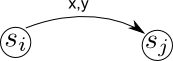
\includegraphics[width=0.3\textwidth]{img_7_1.png} 
	\caption{Representación Diagrama de Estados}
	\end{figure}
	
	Usando el ejemplo anterior, dibujamos el diagrama de estados para $M$.
	%grafico:
	\begin{figure}[h]
	\centering
	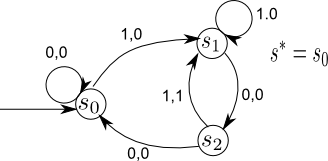
\includegraphics[width=0.5\textwidth]{img_7_2.png} 
	\caption{Diagrama de Estado de $M$}
	\end{figure} 
\end{enumerate}

\section{Sumador Binario}

Sean las cadenas $x,y$

$x=x_5x_4x_3x_2x_1=00111$

$y=x_5y_4y_3y_2y_1=01101$

Un sumador binario en serie es una MEF que nos sirve para hallar x+y.

\textbf{Representación}

%grafico caja
\begin{figure}
\centering
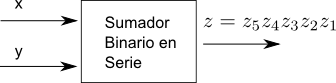
\includegraphics[width=0.5\textwidth]{img_7_3.png} 
\caption{Sumador Binario}
\end{figure}

Para la adición $z=x+y$ tenemos:

$\begin{array}{cccccc}
x=	&0	&0	&1	&1	&1	\\
y=	&0	&1	&1	&0	&1	\\ \hline
	&1	&0	&1	&0	&0
\end{array}$

Podemos modelar este sumador binario mediante una MEF $M$, en la cual.

$S=\{s_0,s_1\}	\qquad \begin{matrix}
s_0 \mbox{ indica un caracter de 0} \\
s_1 \mbox{ indica un caracter de 1}
\end{matrix}$\\

$I=\{00,01,10,11\} \qquad s^*=s_0$

$O=\{0,1\}$

Las funciones $f$ y $g$ quedan definidas en la tabla.

\begin{center}
$\begin{array}{c|cccc|cccc}
S/I	&\multicolumn{4}{c}{f}	&\multicolumn{4}{c}{g}\\
	&00	&01	&10	&11	&00	&01	&10	&11	\\ \hline
s_0	&s_0&s_0&s_0&s_1&0	&1	&1	&0	\\
s_1	&s_0&s_1&s_1&s_1&1	&0	&0	&1
\end{array}$
\end{center}

$$f(s_0,11)=s_1 \qquad g(s_0,11)=0$$

El diagrama de estados para $M$ será (Figura \ref{fig7_4}):

%grafico
\begin{figure}[h]
\centering
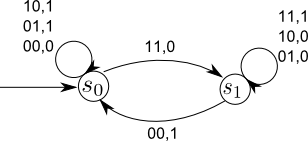
\includegraphics[width=0.5\textwidth]{img_7_4.png} 
\caption{Diagrama de Estados de $M$}\label{fig7_4}
\end{figure}

\textbf{Ejercicio: }Sea $M=(S,I,O,f,g,s^*)$ donde:

$\begin{array}{l}
S=\{s_0,s_1,s_2,s_3\}\\
I=\{a,b,c\} \\
O=\{0,1\}
\end{array}$
\begin{center}
$\begin{array}{c|ccc|ccc}
S/I	&	&f	&	&	&g	&	\\
	&a	&b	&c	&a	&b	&c	\\ \hline
s_0	&s_0&s_3&s_2&0	&1	&1	\\
s_1	&s_1&s_1&s_3&0	&0	&1	\\
s_2	&s_1&s_1&s_3&1	&1	&0	\\
s_3	&s_2&s_3&s_0&1	&0	&1
\end{array}$
\end{center}
Si $s^*=s_0$

\begin{itemize}
\item Obtener la cadena de salida si la entrada es $u=abbccc$.
\item Dibuje el diagrama de estados.
\end{itemize}

\textbf{Solución: }
\begin{center}
$\begin{array}{c|c|c|c|c|c|c}
Estado &s_0	&s_0	&s_3	&s_3	&s_0	&s_2	\\ \hline
Entrada	&a	&b	&b	&c	&c	&c	\\ \hline
Salida	&0	&1	&0	&1	&1	&1
\end{array}$
\end{center}
\begin{align*}
u=abbccc \\
v=101010
\end{align*}

%grafico
\begin{figure}[h]
\centering
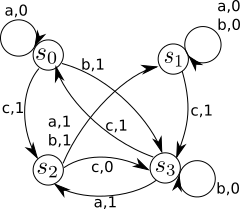
\includegraphics[width=0.4\textwidth]{img_7_5.png}
\caption{Diagrama de Estados}
\end{figure}

\section{Extensión de las funciones $f$ y $g$}

Para una MEF $M=(S,I,O,f,g,s^*)$, la entrada puede ser realizada con un elemento de $I^*$, con la salida $O^*$. Extendemos los dominios de $f$ y $g$ de $S\times I$ a $S\times I^*$.

Para $g$, ampliamos el codominio de $O$ a $O^*$. Con estas extensiones, si $x_1,x_2,x_3...x_k \in I^*$ entonces empezando en cualquier estado $s_1 \in S$ tenemos:
\begin{align*}
f(s_1,x_1)&=s_2	\\
f(s_1,x_1x_2)&=f(f(s_1,s_1),x_2)=f(s_2,x_2)	\\
f(s_1,x_1x_2x_3)&=f(f(\underbrace{f(s_1,x_1)}_{s_2},x_2),x_3)	\\
	&=f(\underbrace{f(s_2,x_2)}_{s_3},x_3)=f(s_3,x_3)	\\
&\vdots	\\
f(s_1,x_1...x_k)&=f(s_k,x_k)=s_{k+1}
\end{align*}

función de estado siguiente extendida.
\begin{align*}
g(s_1,x_1)&=y_1\\
g(s_1,x_1x_2)&=g(s_1,x_1).g(f(s_1,x_1),x_2)\\
&=y_1.g(s_2,x_2)=y_1.y_2\\
g(s_1,x_1x_2x_3)&=g(s_1,x_1).g(s_2,x_2).g(s_3,x_3)\\
&=y_1.y_2.y_3\\
&\vdots\\
g(s_1,x_1...x_k)&=g(s_1,x_1)g(s_2,x_2)...g(s_k,x_k)\\
&=y_1y_2...y_k
\end{align*}

También $f(s_i,\varepsilon)=s_i \qquad \forall s_i \in S$
\chapter{MEF parte II}

\textbf{Definición: }Sea $M=\{S,I,D,f,g,s^*\}$ una MEF.

\begin{enumerate}
\item Para $s_i,s_j\in S$ se dice que $s_j$ es \textbf{alcanzable} desde $s_i$ si $s_i=s_j$ o si hay cadenas de entrada $w\in I^+$ tal que $f(s_i,w)=s$.
\item Un estado $s\in S$ se dice \textbf{transitorio} si $f(s,w)=s$ para $w\in I^* \Rightarrow w=\varepsilon$, es decir, no hay $w\in I^+ /f(s,w)=s$.


\textbf{Ejemplo: }Sea la MEF con diagrama de transición(Figura \ref{img_8_1}).

%imagen
\begin{figure}[h!]
\centering
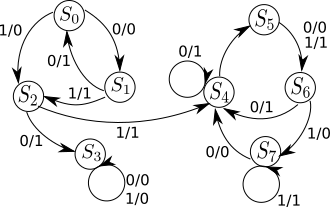
\includegraphics[width=0.35\textwidth]{img_8_1.png}
\caption{Diagrama de Transición}\label{img_8_1}
\end{figure}

\begin{itemize}
\item ¿ Desde qué estados es alcanzable $s_3$?
	
	$s_0,s_1,s_2$
\item ¿ Desde qué estados no es alcanzable $s_3$?

	$s_4,s_5,s_6,s_7$
\item Encuentre un estado transitorio en M.

	$s_2$ es un estado transitorio.
\end{itemize}

\item Un estado $s\in S$ es un estado \textbf{sumidero} si: $f(s,w)=s\qquad \forall w\in I^*$

\item Sea $S_1\in S, \quad I_1 \subseteq I$. Si $ f_1=f|_{S_1\times I_1}$

	$f_1:S_1\times I_1\rightarrow S$ tiene su rango dentro de $S_1$ entonces $g_1=g|_{S_1\times I_1}$
	
	$g_1: S_1\times I_1 \rightarrow O$, entonces $M_1=(S_1,I_1,O_1,f_1,g_1,s^*)$ se llama \textbf{submáquina} de la MEF $M$.
	
\item Una máquina se denomina \textbf{fuertemente conexa} si para cualquier estado $s_i$, $s_j$ es accesible desde $s_i$.

\textbf{Ejemplo: }Usando la MEF anterior.

\begin{itemize}
\item Identifique un estado sumidero.

	$s_3$
\item Encuentre una submáquina.
\begin{itemize}
	\item Sea $s_1=\{s_0,s_1,s_2\}\subseteq S$ y $I_1=\{0,1\}\subseteq I$, 
	$f_1$ tiene algunos estados que caen fuera de $S_1$. ( \xmark )
	
	\item Sea $S_1=\{s_4,s_5,s_6,s_7\}\subseteq S$ y $I=\{0,1\}$ luego $M_1=(S_1,I_1,O,f_1,g_1,s^*)$ es una submáquina de $M$. ( \cmark )
	\item Encuentre una máquina fuertemente conexa.
	
	$M$ no es fuertemente conexa, sin embargo, $M_1$ si es fuertemente conexa.
	
\end{itemize}
\end{itemize}
	

\end{enumerate}

\textbf{Definición: }Para una MEF $M=\{S,I,O,f,g,s^*)$. Sean $s_i,s_j \in S$ dos estados distintos. Una cadena de entrada $w\in I^+$ es llamada \textbf{secuencia de transferencia o transición} desde $s_i$ a $s_j$ si:
\begin{itemize}
\item $f(s_i,w)=s_j$
\item $v\in I^+$ con $f(s_i,v)=s_j\Rightarrow |v|\geq |w|$
\end{itemize}

\textbf{Ejemplo: }Obtener una secuencia de transferencia desde el estado $S_0$ hacia el estado $S_2$ para la MEF $M$ definida sobre $I=\{0,1\}=O$

$S=\{s_0,s_1,s_2,s_3,s_4,s_5,s_6\}$

$M$ está representada por la siguiente tabla.

\begin{center}
$\begin{array}{c|cc|cc}
	&	\multicolumn{2}{c}{f}	&\multicolumn{2}{c}{g}\\
	&0	&1	&0	&1	\\ \hline
s_0	&	s_6		&s_1	&0	&1	\\
s_1	&	s_5		&s_0	&0	&1	\\
s_2	&	s_1		&s_2	&0	&1	\\
s_3	&	s_4		&s_0	&0	&1	\\
s_4	&	s_2		&s_1	&0	&1	\\
s_5	&	s_3		&s_5	&1	&1	\\
s_6	&	s_3		&s_6	&1	&1	\\
\end{array}$
\end{center}

Representamos las transiciones de estado como un árbol(Figura \ref{img_8_2}).

%grafica
\begin{figure}[h!]
\centering
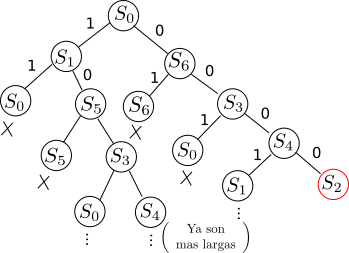
\includegraphics[width=0.4\textwidth]{img_8_2.png}
\caption{Representación como árbol}\label{img_8_2}
\end{figure}

La cadena de transferencia es $w=0000$ con $f(s_0,w)=s_2$ y $g(s_0,w)=0100$. Otra cadena es $v=1000$ pero $|v|>|w|$.

\section{Tipos de MEF}

Para el modelamiento de las calculadoras se ha desarrollado muchos tipos de MEF.

\begin{enumerate}
\item \textbf{Máquina de Moore}
	Una máquina de Moore $M_0=(S,I,O,f,g,s^*)$ es tal que :
\begin{align*}
	S:	&\mbox{ Conjunto de estados}	\\
	I:	&\mbox{ Alfabeto de entrada}	\\
	O:	&\mbox{ Alfabeto de salida}	\\
	f:	&\mbox{ Función de estado siguiente.} f:S\times I\rightarrow S	\\
	g:	&\mbox{ Función de salida, } g:S\rightarrow O	
\end{align*}

\textbf{Representación }\\
\textbf{Ejemplo: }A continuación se presenta la tabla de transición de una máquina de Moore.

\begin{center}
$\begin{array}{c|cc|c}
	&\multicolumn{2}{c|}{f}	&g	\\
S	&a	&b	& 	\\ \hline
s_0	&s_3	&s_2	&0	\\
s_1	&s_1	&s_0	&0	\\
s_2	&s_2	&s_3	&1	\\
s_3	&s_0	&s_1	&0
\end{array}$
\end{center}

Se pide:
\begin{itemize}
\item Dibuje su diagrama de estado.
\item Obtener la cadena de salida para $w=bababbb$
\end{itemize}
\textbf{Solución: }

%grafica
\begin{figure}[h!]
\centering
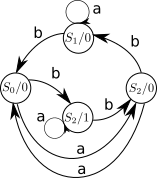
\includegraphics[width=0.2\textwidth]{img_8_3.png}
\caption{Diagrama de Transición}\label{img_8_3}
\end{figure}

\begin{center}
$\begin{array}{c|c|c|c|c|c|c|c}
s_0	&s_2&s_2&s_3&s_0&s_2&s_3&s_1	\\ \hline
b	&a	&b	&a	&b	&b	&b	&		\\ \hline
0	&1	&1	&0	&0	&1	&0	&
\end{array}$
\end{center}

La cadena de salida es $s=0110010$

\item \textbf{Máquina de Mealy: }Fueron estudiados por G.H. Mealy en 1955. En este tipo de máquina las salidas corresponden a transiciones entre estados. Aquí:

\begin{align*}
f:	&S\times I\rightarrow S	\\
g:	&S\times I\rightarrow O
\end{align*}

\textbf{Ejemplo: }Dibuje una máquina de Mealy que imprime el complemento de una cadena de bits de entrada.

\textbf{Solución: }

$S=\{s_0\}$\\
$I=\{0,1\}=O$

\begin{figure}[h!]
\centering
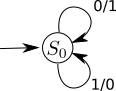
\includegraphics[width=0.15\textwidth]{img_8_4.png}
\caption{Máquina de Mealy}\label{img_8_4}
\end{figure}

\begin{center}
$\begin{array}{c|cc|cc}
	&\multicolumn{2}{c|}{f}	&\multicolumn{2}{c}{g}	\\
	&0	&1	&0	&1	\\ \hline
s_0	&s_0&s_0&1	&0
\end{array}$
\end{center}

\end{enumerate}

\textbf{Teorema: }Si $M_0$ es una máquina de Moore, entonces existe una máquina de Mealy equivalente(Figura \ref{img_8_5}).

\textbf{Método:}
\begin{enumerate}
\item Considere cualquier estado $q_i$ en $M_0$.
\item Suponga que $M_0$ imprime el carácter $t$ al ingresar $q_i$, luego se tiene el rótulo $q_i/t$ en el estado $q_i$.
\item Suponga que hay $n$ arcos de entrada $q_i$ con etiquetas $a_1...a_n$
\item Creamos la máquina de Mealy $M_0$ combinando las etiquetas de los arcos entrantes a $q_i$ a $a_m/t$, $m=1,2,...n$ y cambiamos la etiqueta del estado $q_i/t$ a $q_i$.

%grafico
\begin{figure}[h!]
\centering
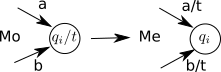
\includegraphics[width=0.30\textwidth]{img_8_5.png}
\caption{Equivalencia entre Mealy y Moore}\label{img_8_5}
\end{figure}
\end{enumerate}
\textbf{Ejemplo: }Convierta la máquina de Moore en la equivalente máquina de Mealy.

%grafico
\begin{figure}[h!]
\centering
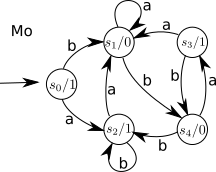
\includegraphics[width=0.25\textwidth]{img_8_6.png}
\caption{Diagrama de Transición}\label{img_8_6}
\end{figure}
%grafico
\begin{figure}[h!]
\centering
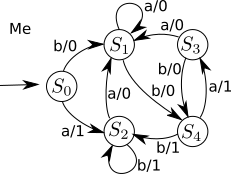
\includegraphics[width=0.25\textwidth]{img_8_7.png}
\caption{Diagrama de Transición}\label{img_8_7}
\end{figure}

\section{MEF sin Salida}
Se usan para el reconocimiento de lenguajes.
\subsection{Autómatas Finitos}

Este tipo de máquinas tienen estados finales y una cadena será reconocida por la máquina si produce una transición desde el estado inicial a una de sus estados finales.

\subsubsection{A.F. Deterministas}
Su salida está limitada a los valores aceptados o rechazados. Formalmente, un $AFD=(S,I,\delta, s^*,F)$
\begin{align*}
	S:	& \mbox{ conjunto finito de estados} (s\not=\phi)	\\
	I:	& \mbox{ alfabeto de entrada}	\\
	\delta:	&\; S\times I\rightarrow S	\\
	F:	& \mbox{ conjunto de estados de aceptacion } (F\subseteq S)	\\
	s^*:	& \mbox{ estado inicial}
\end{align*}

\textbf{Representación: }

Sea el AFD $D$ tal que:
\begin{align*}
S=	&\{s_0,s_1,s_2\}	\\
I=	&\{a,b\}	\\
s^*=	&s_0	\\
F=	&\{s_0\}
\end{align*}
\begin{align*}
\delta(s_0,a)	&=s_1	&\delta(s_0,b)	&=s_2	\\
\delta(s_1,a)	&=s_1	&\delta(s_1,b)	&=s_2	\\
\delta(s_2,a)	&=s_2	&\delta(s_2,b)	&=s_2	
\end{align*}

\textbf{Tabla de Transición: }

\begin{center}
$\begin{array}{c|cc}
	&\multicolumn{2}{c}{\delta}	\\
	&a	&b	\\ \hline
\sharp s_0	&s_1&s_2	\\
s_1	&s_1&s_2	\\
s_2	&s_2&s_2
\end{array}$
\end{center}

\textbf{Diagrama de Transición: }

%grafico
\begin{figure}[h!]
\centering
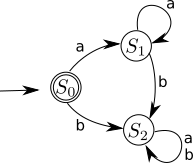
\includegraphics[width=0.25\textwidth]{img_8_8.png}
\caption{Diagrama de Transición de $D$}\label{img_8_8}
\end{figure}

$w=babb$ no es aceptada por $D$.

$F=\{s_1\}$
\begin{figure}[h!]
\centering
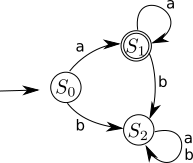
\includegraphics[width=0.25\textwidth]{img_8_9.png}
\caption{Diagrama de Transición}\label{img_8_9}
\end{figure}
\begin{align*}
\left. \begin{array}{c}
	u_1	=a	\\
	u_2	=aa	\\
	\vdots	\\
	u_n	=a^n
	\end{array}\right \} \mbox{Son aceptados por D}
\end{align*}
En el autómata Fig \ref{img_8_9}. Este autómata acepta cadenas formadas solo por $a$. El estado  $s_2$ es un estado \textbf{muerto}.

\textbf{Estado Muerto: }Es aquel estado que no es de aceptación y no parte de él ninguna transición hacia otro estado.

\textbf{Nota: }El AF $D$ se llama determinístico porque el $(s_2)$ estado siguiente queda bien definido (es único) si son conocidos el estado $(s_1)$ y el símbolo $(a)$:
$$\delta(s_1,a) = s_2$$

\section{Autómatas Incompletos}
En algunas ocasiones podemos encontrar autómatas donde no estén definidas todas las transiciones.

Si una cadena hace llegar al AFD a una situación no definida, se asumirá que la cadena no ha sido reconocido por el autómata.

\chapter{AFD parte II}
\textbf{Ejemplo: }Del ejemplo de la anterior clase.
%grafico1
\begin{figure}[h!]
\centering
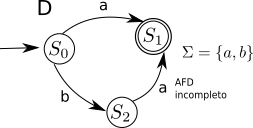
\includegraphics[width=0.4\textwidth]{img_9_1.png}
\caption{AFD incompleto}\label{img_9_1}
\end{figure}


Para que el autómata $D$ se vuelva completo se debe añadir un estado muerto.

%grafico2
\begin{figure}[h!]
\centering
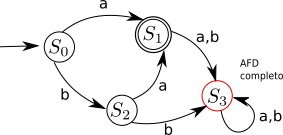
\includegraphics[width=0.4\textwidth]{img_9_2.png}
\caption{AFD completo}\label{img_9_2}
\end{figure}

\textbf{Definición: }Un AFD es conexo si todos sus estaso son accesibles desde el estado inicial.

\textbf{Definición: }En un autómata que no es conexo, se llamará la \textbf{parte conexa} del autómata al conjuto de estados accesibles desde el estado inicial.

\textbf{Ejemplo: }Dibuje un AFD no conexo y determine su parte conexa.
%grafico3
\begin{figure}[h!]
\centering
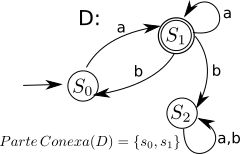
\includegraphics[width=0.4\textwidth]{img_9_3.png}
\caption{Diagrama AFD $D$}\label{img_9_3}
\end{figure}

\textbf{Definición: }Sea un AFD $D=(S,I,\delta,s^*,F)$, llamaremos función de transición extendida a $\widehat{\delta}$ que actúa no solo sobre símbolos sino sobre cadena de símbolos. $\widehat{\delta}$ la definimos recursivamente como sigue:
\begin{enumerate}
\item $\widehat{\delta}(s;\varepsilon)=S \qquad \forall s\in S$
\item (parte recursiva) $\widehat{\delta}(s,au) = \widehat{\delta}(\delta(s,a),u)\qquad a\in \Sigma^* \qquad u\in I^*$

OBS: Notar que $\widehat{\delta}(s,a)=\delta(s,a)$
\begin{align*}
\widehat{\delta}(s,a)&=\widehat{\delta}(s,a.\varepsilon)	\\
				&=\widehat{\delta}(\downlegend{\delta(s,a)}{Estado sgte},\varepsilon) \\
				&=\delta(s,a)
\end{align*}
\end{enumerate}

\textbf{Ejemplo: }Para el AFD $D$

%grafico4
\begin{figure}[h!]
\centering
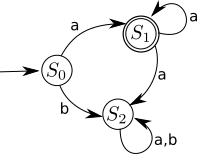
\includegraphics[width=0.3\textwidth]{img_9_4.png}
\caption{Diagrama de Transición de $D$}\label{img_9_4}
\end{figure}
Obtener:
\begin{itemize}
\item $\widehat{\delta}(s_0,a)$
\item $\widehat{\delta}(s_0,ab)$
\item $\widehat{\delta}(s_0,baba)$
\end{itemize}
Usaremos la evaluación rápida.

\textbf{Solución: }
\begin{itemize}
\item $\widehat{\delta}(s_0,a)=\delta(s_0,a)=s_1$

	$s_0\xrightarrow{a} \underline{s_1}$
\item $\widehat{\delta}(s_0,ab)=s_2$

	$s_0\xrightarrow{a}s_1\xrightarrow{b}\underline{s_2}$
\item $\widehat{\delta}(s_0,baba)=s_2$

camino: $s_0\xrightarrow{b}s_2\xrightarrow{a}s_2\xrightarrow{b}s_2\xrightarrow{a}\underline{s_2}$
\end{itemize}
\textbf{Ejemplo: }Sea el AFD $D$, con $\Sigma=\{0,1\}$.

%grafico5
\begin{figure}[h!]
\centering
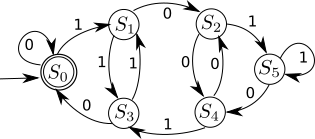
\includegraphics[width=0.4\textwidth]{img_9_5.png}
\caption{Diagrama de Transición de $D$}\label{img_9_5}
\end{figure}

Donde $s^*=s_0$, $F=\{s_0\}\rightarrow\mbox{estado de aceptación}$

Obtener: $\widehat{\delta}(s_0,w)$ para $w=1010$, usando la definición recursiva.
\begin{align*}
\widehat{\delta}(s_0,\downlegend{1}{a}\underbrace{010}_{u})&=\widehat{\delta}(\delta(s_0,1),010)	\\
				&=\widehat{\delta}(s_1,\downlegend{0}{a}\underbrace{10}_{u})	\\
				&=\widehat{\delta}(\delta(s_1,0),10)	\\
				&=\widehat{\delta}(s_2,\downlegend{1}{a}\downlegend{0}{u})	\\
				&=\widehat{\delta}(\delta(s_2,1),0)	\\
				&=\widehat{\delta}(s_5,0)	\\
				&=\delta(s_5,0)	\\
				&= s_4
\end{align*}

$w$ no es aceptada por $D$, para ser aceptada debió acabar en $s_0$.

\textbf{Definición: }El lenguaje reconocido por un autómata $D=(S,I,\delta,s^*,F)$ es el conjunto:
$$L(D)=\{ w\in I^*/\widehat{\delta}(s^*,w)\in F\}$$

Son todas las cadenas aceptadas por el autómata.

\textbf{Ejemplo: }Identifique los elementos del AFD $D$ cuyo lenguaje está dado por el siguiente conjunto:
$$L(D)=\{ w\in I^*/ w \mbox{ tiene un número par de símbolos}\}$$
$$I=\{0,1\}$$

Para el autómata $D=(S,I,\delta,s^*,F)$ se tiene: 
\begin{align*}
I=&\{0,1\}	\\
S=&\{S_{par},S_{impar}\}	\\
F=&\{S_{par}\} \qquad \rightarrow\mbox{Estado de aceptación}	\\
s^*= &S_{par}
\end{align*}
Su tabla de transición será:
\begin{center}
\begin{tabular}{r|cc}
	&\multicolumn{2}{c}{$\delta$}	\\
+	&0		&1	\\ \hline
$(*)\rightarrow S_{par}$	&$S_{impar}$	&$S_{impar}$	\\
$S_{impar}$	&$S_{par}$	&$S_{par}$

\end{tabular}
\end{center}
(*):Tenemos longitud de cadena par + $0$ =$S_{impar}$

Su diagrama de estados:

%grafica6
\begin{figure}[h!]
\centering
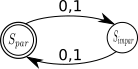
\includegraphics[width=0.2\textwidth]{img_9_6.png}
\caption{Diagrama de Transición de $D$}\label{img_9_6}
\end{figure}

\textbf{Ejemplo: }Identifique los elementos del AFD $D$ que reconoce el lenguaje:
$$L(D)=\{w\in I^*/ w \mbox{ tiene un número}\overbrace{\mbox{ par de 0's}}^{P}\mbox{ y un número} \underbrace{\mbox{impar de 1's}}_{P}\}$$

Dibuje su tabla y diagrama de transición, $I=\{0,1\}$.
\begin{align*}
s^*=&PP	\\
S=&\{\uplegend{P}{(1)}\uplegend{P}{(2)},\downlegend{P}{(3)}\downlegend{I}{(4)},IP,II\}	\\
F=&\{PP\}
\end{align*}
(1):par de 0's; (2):par de 1's; (3):par de 0's; (4):impar de 1's.

Donde:
\begin{itemize}
\item PP: cantidad par de ceros y cantidad par de unos.
\item PI: cantidad par de ceros y cantidad impar de unos.
\item IP: cantidad impar de ceros y cantidad par de unos.
\item II: cantidad impar de ceros y cantidad impar de unos.
\end{itemize}

\begin{center}
\begin{tabular}{c|cc}
	&\multicolumn{2}{c}{$\delta$}\\
+	&0	&1	\\ \hline
$(*)\rightarrow$PP	&IP	&PI	\\
PI	&II	&PP	\\
IP	&PP	&II	\\
II	&PI	&IP	
\end{tabular}
\end{center}
(*): PP le aumentamos $0$ y quedaría cantidad impar de ceros, 1's no varían.

Diagrama:

%grafico7
\begin{figure}[h!]
\centering
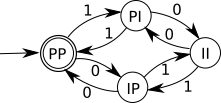
\includegraphics[width=0.4\textwidth]{img_9_7.png}
\caption{Diagrama de Transición de $D$}\label{img_9_7}
\end{figure}

\section{Minimización de un AFD}

\textbf{Definición: }Dos estados $s_1,s_2\in S$ se dirán equivalentes, denotándolos por $s_1\simeq s_2$, si $\forall w\in I^*$:
$$\widehat{\delta}(s_1,w)\in F \Leftrightarrow \widehat{\delta}(s_2,w)\in F$$

Es decir las transiciones que parten de ellos para cada uno de los símbolos del alfabeto llevan al mismo estado $0$ a estados que son equivalentes entre si:

\textbf{Definición: }Un AFD $D$ se llamará autómata mínimo para el lenguaje $L(D)$ si ningún AFD $M$ para $L(M)$ contiene un menor número de estados que $D$.

\section{Algoritmo de Minimización de Estados de un AFD}

\textbf{Objetivo: } Agrupar estados equivalentes para conseguir un AFD equivalente al original.

Pasos:
\begin{enumerate}
\item Vamos a construir una partición $\pi$ de $S$ formada por dos componentes: los estados de aceptación y los que no son.
\item Refinar la partición separando en diferentes componentes a los estados que no son equivalentes.
\item Terminar cuando cada componente de la partición, agrupa estados equivalentes.
\end{enumerate}

\textbf{Ejemplo: }Minimizar el AFD $D$ siguiente(Figura \ref{img_9_8}):

%grafico8
\begin{figure}[h!]
\centering
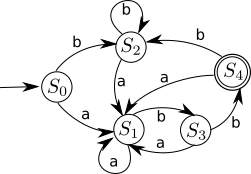
\includegraphics[width=0.4\textwidth]{img_9_8.png}
\caption{Diagrama de Transición de $D$}\label{img_9_8}
\end{figure}

$$\Sigma=\{a,b\} \qquad, s^*=s_0$$

\textbf{Solución: }Tenemos $I=\{a,b\}; S=\{s_0,s_1,s_2,s_3,s_4\}; F=\{s_4\}$.

\begin{enumerate}
\item Construimos $\pi=\{P_1,P_2\}$
\begin{align*}
P_1=&\{s_4\} \\
P_2=&\{s_0,s_1,s_2,s_3\}
\end{align*}
Evaluamos $P_2$ en $I$
\begin{center}
\begin{tabular}{c|cl}
	&\multicolumn{2}{c}{$\delta$}\\
	&a	&b	\\ \hline
$s_0$	&$s_1\in P_2$	&$s_2\in P_2$	\\
$s_1$	&$s_1\in P_2$	&$s_3\in P_2$	\\
$s_2$	&$s_1\in P_2$	&$s_2\in P_2$	\\
$s_3$	&$s_1\in P_2$	&$s_4\not\in P_2,\in P_1\rightarrow (*)$
\end{tabular}
\end{center}
(*): No es estado equivalente. $s_3$ no es equivalente a los estados $s_0,s_1,s_2$.

\item Refinamos la partición $\pi=\{P_1,P_2,P_3\}$
$$P_1=\{s_4\},\qquad P_2=\{3\},\qquad P_3=\{s_0,s_1,s_2\}$$
Analizamos $P_3$ en $I$.
\begin{center}
$\begin{array}{c|cl}
	&a	&b	\\ \hline
s_0	&s_1\in P_3	&s_2\in P_3	\\
s_1	&s_1\in P_3	&s_3\in P_2\rightarrow (1)	\\
s_2	&s_1\in P_3	&s_2\in P_3

\end{array}$
\end{center}
(1): No es estado equivalente. $s_1\not\simeq s_0,s_2$.
\item Refinamos la partición $\pi=\{P_1,P_2,P_3,P_4\}$.
$$P_1=\{s_4\},\qquad P_2=\{s_3\},\qquad P_3=\{s_1\},\qquad P_4=\{s_0,s_2\}$$
Analizamos $P_4$ en $I$.
\begin{center}
$\begin{array}{c|cc}
	&a	&b \\ \hline
s_0	&s_1\in P_3	&s_2\in P_4	\\
s_2	&\underbrace{s_1\in P_3}_{Equivalencia}	&\underbrace{s_2\in P_4}_{Equivalencia}
\end{array}$
\end{center}
Ya no es posible hacer mas refinamientos.

%grafico9
\begin{figure}[t!]
\centering
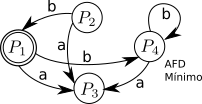
\includegraphics[width=0.4\textwidth]{img_9_9.png}
\caption{Diagrama de Transición del AFD $D$ mínimo}\label{img_9_9}
\end{figure}
\end{enumerate}

\chapter{Minimización de AFD}

\section{Minimización de un AFD. AFD equivalentes}

\textbf{Definición: }Dos AFD definidos sobre un alfabeto $I$, se dice equivalentes si ambos reconocen el mismo lenguaje.

Formalmente:

$D_1$ es equivalente a $D_2$ sobre $I$ si $L(D_1)=L(D_2)$

\section{Método de Comprobación}

Sean los autómatas $D_1=(S_1,I,\delta_1,s_1^*,F_1)$ y $D_2=(S_2,I,\delta_2,s_2^*,F_2)$

\begin{enumerate}
\item Unirlos en un único autómata determinista de modo que no sea conexo, como sigue:

$D=D_1\cup D_2=(S_1\cup S_2,I,\delta,s^*,F_1\cup F_2)$

donde :

$\delta(s,a)=\left\{ \begin{array}{ll} 
\delta_1(s,a) 	&	s\in S_1	\\
\delta_2(s,a)	& 	s\in S_2	\end{array}\right.$

Para $s^*$, podemos elegir $s_1^*$ o $s_2^*$

\item Minimizar el autómata AFD $D$.
\item Si se verifica que los estados iniciales $s_1^*$ y $s_2^*$ son equivalentes diremos que $D_1$ y $D_2$ lo son.

\end{enumerate}

\textbf{Ejemplo: }Sean los AFD $D_1$ y $D_2$ representados por su diagrama de transición(Figura \ref{img_10_1} y \ref{img_10_2}):

%Grafico1
\begin{figure}[h!]
\centering
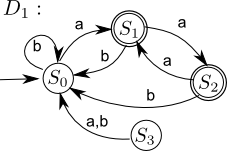
\includegraphics[width=0.3\textwidth]{img_10_1.png}
\caption{Diagrama de transición $D_1$}\label{img_10_1}
\end{figure}

$I=\{a,b\}$
%Grafico2
\begin{figure}[h!]
\centering
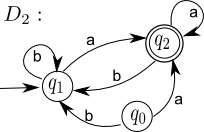
\includegraphics[width=0.3\textwidth]{img_10_2.png}
\caption{Diagrama de transición $D_2$}\label{img_10_2}
\end{figure}

\begin{center}
$\begin{array}{lp{1cm}l}
\mbox{Para }D_1:&			&\mbox{Para }D_2:	\\
S_1=\{s_0,s_1,s_2,s_3\}&		&S_2=\{q_0,q_1,q_2\}\\
s_1^*=s_0&					&s_2^*=q_1	\\
F_1=\{ s_1,s_2\}&			&F_2^=\{q_2\}
\end{array}$
\end{center}

Para $D$: 
\begin{align*}
S=&\{s_0,s_1,s_2,s_3,q_0,q_1,q_2\}\\
F=&\{s_1,s_2,q_2\}
\end{align*}

Minimizamos $D$:

Se tiene $\pi =\{P_1,P_2\}$, donde:
\begin{align*}
P_1=&\{s_1,s_2,q_2\}\mbox{	y}\\
P_2=&\{s_0,s_3,q_0,q_1\}
\end{align*}

Evaluamos $P_1$ para cada símbolo de $I$.

\begin{center}
\begin{tabular}{c|cc}
		&\multicolumn{2}{c}{$\delta$}	\\
$S\backslash I$	&$a	$			&$b$			\\ \hline
$s_1$	&$s_2\in P_1$	&$s_0\in P_2$	\\
$s_2$	&$s_1\in P_1$	&$s_0\in P_2$	\\
$q_2$	&$\downlegend{q_2\in P_1}{estados  equivalentes}$	&$q_1\in P_2$
\end{tabular}
\end{center}

Evaluamos $P_2$ para cada símbolo de $I$.

\begin{center}
\begin{tabular}{c|ccl}
		&\multicolumn{2}{c}{$\delta$}	\\
$S\backslash I$	&$a$	&$b$	&\\ \hline
$s_0$	&$s_1\in P_1$	&$s_0\in P_2$ &	\\
$s_3$	&$s_0\in P_2$	&$s_0\in P_2$ &$\rightarrow$ **	\\
$q_0$	&$q_2\in P_1$	&$q_1\in P_2$ &	\\
$q_1$	&$q_2\in P_1$	&$q_1 \in P_2$ &

\end{tabular}
\end{center}

**: No es equivalente al resto.

Refinamos la partición $\pi=\{P_1,P_2,P_3\}$
\begin{align*}
\alpha \left \{
\begin{array}{ll}
P_1=	&	\{s_1,s_2,q_2\}	\\
P_2=	&	\{s_3\}\rightarrow \mbox{este es equivalente a si mismo} \\
P_3=	&	\{s_0,q_0,q_1\}
\end{array}\right.
\end{align*}

Evaluamos $P_3$ para cada símbolo de $I$(miramos D aún), comparamos con $\alpha$.
\begin{center}
\begin{tabular}{c|cc}
				&\multicolumn{2}{c}{$\delta$}	\\
$S\backslash I$	&$a$			&$b$			\\ \hline
$s_0$			&$s_1\in P_1$	&$s_0\in P_3$	\\
$q_0$			&$q_2\in P_1$	&$q_1\in P_3$	\\
$q_1$			&$q_2\in P_1$	&$q_1\in P_3$	
\end{tabular}
\end{center}
Todos son equivalentes.

Así que ya no refinamos. Además en $P_3$, $s_0,q_1$ son equivalentes, luego $D_1$ y $D_2$ son equivalentes. El autómata equivalente a $D_1$ y $D_2$ es(Figura \ref{img_10_3}):
\begin{figure}[h!]
\centering
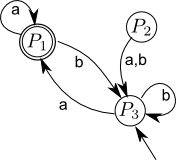
\includegraphics[width=0.3\textwidth]{img_10_3.png}
\caption{Diagrama de transición $D$}\label{img_10_3}
\end{figure}
Para el estado inicial, veo en que conjunto está incluido y ese será mi estado inicial. Veo elementos de $P_2$, y veo con que símbolo está en la primera gráfica, luego veo donde cae o (estado siguiente) y ese estado veo en que conjunto final está.

\begin{align*}
\left. \begin{array}{c}
aba \; \checkmark \\
bba \; \checkmark \end{array}\right \} \mbox{acepta} \rightarrow \mbox{pero no pasa por } P_2
\end{align*}

Se identifica que $P_2$ es un estado inaccesible, luego podemos retirarlo(Figura \ref{img_10_4}).
\begin{figure}[h!]
\centering
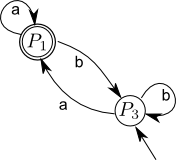
\includegraphics[width=0.3\textwidth]{img_10_4.png}
\caption{Autómata Finito Simplificado}\label{img_10_4}
\end{figure}

En un AFD: $\delta( \downlegend{s_1}{(1)},\downlegend{a}{(2)})=\downlegend{s_2}{(3)}$

donde: $\begin{array}{cl}
			(1)	& 	\mbox{Estado actual} \\
			(2)	&	\mbox{Símbolo}	\\
			(3)	&	\mbox{Estado siguiente}
\end{array}$

\section{Autómatas Finitos No Deterministas}

Si la condición que existe una única transición para el par $(s,a)$ se elimina, es decir, si para algún par $(s,a)$ hubiera transiciones hacia dos o más estados se tiene lo que se denomina, un autómata no determinístico \textbf{(AFND)}.

\begin{figure}[h!]
\centering
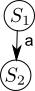
\includegraphics[width=0.05\textwidth]{img_10_5.png}
\caption{AFD}\label{img_10_5}
\end{figure}

\begin{figure}[h!]
\centering
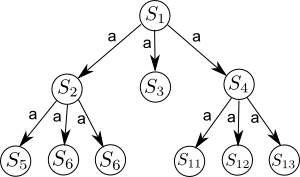
\includegraphics[width=0.5\textwidth]{img_10_6.png}
\caption{AFND}\label{img_10_6}
\end{figure}

\textbf{Definición: }Un autómata FND, $N=(S,I,\delta,s^*,F)$. $S,I,s^*$ y $F$ se definen del mismo modo que en los AFD.

\begin{center}
$\begin{array}{ll}
\delta:	&\mbox{regla de transición}	\\
\delta:	& S\times I \rightarrow P(s)	\\
P(s)	&\mbox{incluye a } \phi
\end{array}$
\end{center}

Como $\delta$ asigna a cada par de estado y símbolo, un conjunto de estados, se le denomina relación de transición.

\subsection{Representaciones para un AFND}

\begin{enumerate}
\item Tabla de transición:
	Sea el AFND $N$, donde:
	
	$\begin{array}{ll}
	S=	&\{s_0,s_1,s_2\}	\\
	I=	&\{a,b\}\rightarrow **	\\
	s^*=&s_0	\\
	F=&\{s_0\}	
	\end{array}$
	
	**: Cada estado debe tener dos salidas(normalmente). en este caso(AFND) no se cumple.
	
\textbf{Ejemplo: } Si: 

$\begin{array}{ll}
	\delta(s_0,a)=	&\{s_1\}	\\
	\delta(s_1,b)=	&\{s_0,s_2\}	\\
	\delta(s_2,a)=	&\{s_0\}
\end{array}$

Dibuje la tabla de transición:

\begin{center}
\begin{tabular}{r|cl}
	&$a$	&$b$	\\ \hline
$(1)\rightarrow \#s_0$	&$\{s_1\}$	&$\phi$	\\
$s_1$		&$\phi$	&$\{s_0,s_2\}$	\\
$s_2$		&$\{s_0\}$	&$\phi\rightarrow (2)$	
\end{tabular}
\end{center}

(1): Estado de aceptación; (2):Si no me dan información se pone $\phi$.
\item Diagrama de Transición:

\begin{figure}[h!]
\centering
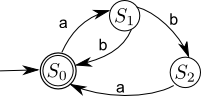
\includegraphics[width=0.3\textwidth]{img_10_7.png}
\caption{Diagrama de Transición}\label{img_10_7}
\end{figure}

\textbf{Ejercicio: }Halle el D.T del AFND siguiente:
\begin{center}
\begin{tabular}{r|cc}
	&$0$	&$1$	\\ \hline
$\rightarrow s_0$	&$\{s_0,s_1\}$	&$\{s_3\}$	\\
$s_1$				&$\{s_0\}$		&$\{s_1,s_3\}$\\
$\#s_2$				&$\{\phi\}$		&$\{s_0,s_2\}$\\
$\#s_3$				&$\{s_0,s_1,s_2\}$&$\{s_1\}$
\end{tabular}
\end{center}

\begin{figure}[h!]
\centering
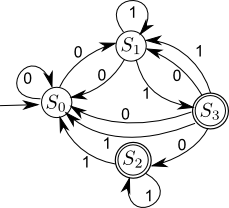
\includegraphics[width=0.3\textwidth]{img_10_8.png}
\caption{Diagrama de Transición}\label{img_10_8}
\end{figure}
\end{enumerate}

\textbf{Ejemplo: }Considere AFND: $N=(S,I,\delta,s^*,F)$. Procesemos la cadena $w=aba$, $s^*=s_0$

\begin{center}
$\begin{array}{cl}
\delta(s_0,a)=	&s_1	\\
\delta(s_1,b)=	&s_2 \rightarrow \mbox{Elijo }\{s_0,s_2\}	\\
\delta(s_2,a)=	&s_0 \rightarrow \mbox{estado de aceptación}
\end{array}$
\end{center}

Al ser $\delta(s_1,b)=s_0$ y $\delta(s_0,a)=s_1 \rightarrow w$ no es aceptada.

Pero si hay un camino que $w$ si es aceptada entonces $w$ es aceptada por AFND. $w$ es aceptada por AFND $N$.

En un modelo de computación no determinista se asume que siempre se hace la elección correcta.

\textbf{Definición: }Sea un AFND $N=(S,I,\delta,s^*,F)$. La regla de transición extendida para $N$ es una relación de $P(s)\times I^*$ hacia $P(s)$, la cual se define de forma recursiva como sigue:

\begin{itemize}
\item $\widehat{\delta}(\phi,w)=\phi$, $\forall w\in I^*$
\item $\widehat{\delta}(A,\varepsilon)=A$,  $\forall A\subseteq S$
\item $\widehat{\delta}(A,au)=\widehat{\delta}\left(\bigcup_{s\in A}\delta(s,a),u\right)$,  $A\subseteq S, a\in I, u\in I^*$

En particular cuando $w=a$ y $A\not= \phi$.
\begin{align*}
\widehat{\delta}(A,a)&=\widehat{\delta}(A,a.\varepsilon)	\\
	&=\widehat{\delta}\downlegend{\left(\bigcup_{s\in A}\delta(s,a)\varepsilon\right)}{$B=\{s_1\cup s_2\cup s_3\}$}, \\
	&=\bigcup_{s\in A}\delta(s,a)
\end{align*}
\end{itemize}

\textbf{Ejemplo: }Dado el AFND, $N$ donde:
\begin{align*}
S=&\{s_0,s_1\}	\\
I=&\{0,1\}	\\
s^*=&s_0	\\
F=&\{s_1\}
\end{align*}
\begin{center}
\begin{tabular}{c|cc}
	&$0$	&$1$	\\ \hline
$\rightarrow s_0$	&$\{s_0,s_1\}$	&$\{s_0\}$	\\
$\#s_1$	&$\phi$		&$\phi$
\end{tabular}
\end{center}
Use la función recursiva y determine si $w=1010$ es aceptada o no por $N$ en $I=\{0,1\}$.

\begin{align*}
\widehat{\delta}(\{\underbrace{s_0}_{A}\},\uplegend{1}{a}\overbrace{1010}^{u}) &=\widehat{\delta}(\delta(s_0,1),010)	\\
					  &=\widehat{\delta}(\{s_0\},\uplegend{0}{a}\overbrace{10}^{u})\\
					  &=\widehat{\delta}(\delta(s_0,0),10)	\\
					  &=\widehat{\delta}(\{s_0\},10)	\\
					  &=\widehat{\delta}(\delta(s_0,1),0)	\\
					  &=\widehat{\delta}(\{s_0\},0)	\\
					  &=\delta(\{s_0\},0)	\\
					  &=\{s_1,s_0\}
\end{align*}

Si es estado de aceptación, entonces $w$ es aceptada por $N$.

\textbf{Definición: }El lenguaje reconocido por un AFND $N$ es el conjunto:
$$L(N)=\{ w\in I^* / \widehat{\delta}(\{s^*\}, w)\cap F\not= \phi\}$$

Para afirmar que una cadena no está en $L(N)$ debemos agotar todas las posibilidades (formas posibles) de recorrer el diagrama de transición para dicha cadena.

\chapter{Autómatas con Transiciones Epsilon}
Extenderemos la definición de los AFND para incluir transiciones de un estado a otro que no dependen de ninguna entrada.

\textbf{Notación: }AFND-$\varepsilon$

\textbf{Definición: }Formalmente un AFND-$\varepsilon$ es una quíntupla $N=(S,I,\delta,s^*,F)$ donde $S,I,s^*,F$ se definen como en los AFND. $\delta$ es una función total de $(S\times I \cup\{\varepsilon\} \rightarrow P(s))$\\

\textbf{Ejemplo: }El siguiente AFND-$\varepsilon$ (Figura \ref{img_11_1}), $I=\{0,1,2\}$

%grafico1
\begin{figure}[h!]
\centering
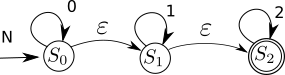
\includegraphics[width=0.5\textwidth]{img_11_1.png}
\caption{Diagrama de Transición} \label{img_11_1}
\end{figure}
$$L(N)=\{0^m1^n2^p/m\geq0,n\geq 0,p\geq 0\}$$

\textbf{Ejemplo: }Averiguar si la cadena $w=002$ es aceptada por el AFND-$\varepsilon$ $N$ (Figura \ref{img_11_1}), usando la definición recursiva.

\begin{align*}
\widehat{\delta}(s_0,\downlegend{0}{a}\downlegend{02}{u}) &=\widehat{\delta}(\delta(s_0,0),\downlegend{0}{a}\downlegend{2}{u})=\widehat{\delta}(s_0,02)=\widehat{\delta}(\delta(s_0,0),2) \\
&=\widehat{\delta}(s_0,\downlegend{2}{$\varepsilon 2$})=\widehat{\delta}(\delta(s_0,\varepsilon),2)=\widehat{\delta}(s_1,\downlegend{2}{$\varepsilon 2$})=\widehat{\delta}(\delta(s_1,\varepsilon),2)\\
&=\widehat{\delta}(s_2,2)=\delta(s_2,2)=s_2
\end{align*}

$w$ es aceptado por $N$, pues $s_2\in F$.

El camino que va de $s_0$ hacia $s_2$ es: 
$$s_0\rightarrow \downlegend{s_0}{0}\rightarrow \downlegend{s_0}{0}\rightarrow \downlegend{s_1}{$\varepsilon$}\rightarrow \downlegend{s_2}{$\varepsilon$} \rightarrow \downlegend{s_2}{2}$$

\textbf{Representación de un AFND}-$\varepsilon$: $\delta$ toma un estado de $S$ y un elemento de $I\cup \{\varepsilon\}$.

\textbf{Ejemplo: }Dibuje la tabla de transición para $N$
\begin{center}
$\begin{array}{c|cccc}
s		&0		&1		&2		& \varepsilon	\\ \hline
s_0		&s_0	&\phi	&\phi	&s_1	\\
s_1		&\phi	&s_1	&\phi	&s_2	\\
\sharp s_2	&\phi	&\phi	&s_2	&\phi
\end{array}$
\end{center}

\textbf{Definición: }Para todo estado $s\in S$ definimos la $\varepsilon$-clausura de $s$ como:
$$clausura_\epsilon(s)=\{ q/q \mbox{ es accesible desde }s\mbox{ sin consumir nada en la entrada} \}$$

\textbf{Nota: }El estado $s$ pertenece a $clausura_\epsilon(s)$.

\textbf{Ejemplo: }En el AFND-$\varepsilon$ $N$ (Figura \ref{img_11_1}) determine la clausura $\varepsilon$ para:

\begin{itemize}
\item $s=s_0$
\item $s=s_1$
\item $s=s_2$
\end{itemize}
\textbf{Solución: }
\begin{itemize}
\item $clausura_\varepsilon(s_0)=\{s_0,s_1,s_2\}$
\item $clausura_\varepsilon(s_1)=\{s_1,s_2\}$
\item $clausura_\varepsilon(s_2)=\{s_2\}$
\end{itemize}

Podemos extender la $\varepsilon$-clausura a un conjunto de estados $Q$ como sigue:
\begin{align*}
clausura_\varepsilon(Q)&=\bigcup_{q\in Q}clausura_\varepsilon(q)\\
clausura_\varepsilon(\{q_1,q_2,...,q_{i_N}\})&= \bigcup_{k=1}^N clausura_\varepsilon(q_{i_k})\\
Q\subseteq S
\end{align*}

\textbf{Ejemplo: }Dado el siguiente diagrama (Figura \ref{img_11_2}):

%grafico2
\begin{figure}[h!]
\centering
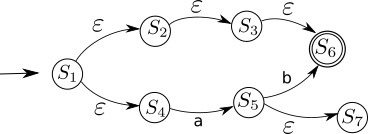
\includegraphics[width=0.5\textwidth]{img_11_2.png}
\caption{Diagrama de Transición} \label{img_11_2}
\end{figure}
Determine:
\begin{itemize}
\item $clausura_\varepsilon(s_1)$
\item El camino seguido para llegar a cada estado
\end{itemize}
\textbf{Solución: }
\begin{itemize}
\item $clausura_\varepsilon(s_1)=\{s_1,s_2,s_3,s_4,s_6\}$
\item
$\begin{array}{c|c}
s	&\mbox{camino}	\\ \hline
s_1	&s_1	\\
s_2	&s_1\rightarrow s_2	\\
s_3	&s_1\rightarrow s_2\rightarrow s_3	\\
s_4	&s_1\rightarrow s_4	\\
s_6	&s_1\rightarrow s_2\rightarrow s_3\rightarrow s_6
\end{array}$
\end{itemize}

\textbf{Definición: }La función de transición extendida a cadenas $\widehat{\delta}$ se define recursivamente:
\begin{itemize}
\item $\widehat{\delta}(s,\varepsilon)=clausura_\varepsilon(s)$
\item $\widehat{\delta}(s,ua)=clausura_\varepsilon(Q)$ Donde:

	$Q=\{q/\exists r\in \widehat{\delta}(s,u)\land q\in \delta(r,a)\}$
	
	$a\in I;u\in I^*;r,s\in S$ %%revisar
\end{itemize}

\textbf{Definición: }El lenguaje aceptado por un AFND-$\varepsilon$ $N=(S,I,\delta,s^*,F)$ es el conjunto.
$$L(N)=\{w/\widehat{\delta}(s^*,w)\land F\not= \phi\}$$

\textbf{Ejemplo: }Determine si $N$ acepta a la cadena $w=01$ en (Figura \ref{img_11_1}).

\textbf{Solución: }Hallamos primero $\widehat{\delta}(s_0,\varepsilon)$ y $\widehat{\delta}(s_0,0)$, $F=\{s_2\}$.
\begin{itemize}
\item $\widehat{\delta}(s_0,\varepsilon)=clausura_\varepsilon(s_0)=\{s_0,s_1,s_2\}$
\item \begin{align*}
\widehat{\delta}(s_0,\underbrace{0}_{\varepsilon 0})&=clausura_\varepsilon(\delta(\widehat{\delta}(s_0,\underbrace{\varepsilon}_{u}),\underbrace{0}_{a}))\\
&=clausura_\varepsilon(\delta(\{\underbrace{s_0,s_1,s_2}_{Q}\},0))\\
&=clausura_\varepsilon(\delta(s_0,0)\cup \delta(s_1,0)\cup \delta(s_2,0))\\
&=clausura_\varepsilon(s_0)=\{s_0,s_1,s_2\}
\end{align*}
Así:
\begin{align*}
\widehat{\delta}(s_0,\underbrace{0}_{u}\underbrace{1}_{a})&=clausura_\varepsilon(\delta(\widehat{\delta}(s_0,0),1))\\
&=clausura_\varepsilon(\delta(\{\underbrace{s_0,s_1,s_2}_{Q}\},1))\\
&=clausura_\varepsilon(\underbrace{\delta(s_0,1)}_{\phi}\cup \underbrace{\delta(s_1,1)}_{s_1}\cup \underbrace{\delta(s_2,1)}_{\phi})\\
&=clausura_\varepsilon(s_1)=\{s_1,s_2\}
\end{align*}
Como $\{s_1,s_2\}\cap F=\{s_2\}$, se acepta $w$.
\end{itemize}

\textbf{Definición: }Se define el conjunto de estado que siguen a $p$, pasando  por $\sigma$, mediante:
$$d(p,\sigma)=\{q/\mbox{hay una transición de }p\mbox{ a }q\mbox{ etiquetada por  }\sigma\}\qquad \sigma\in I$$

\textbf{Extensión}
$$d(\{\underbrace{p_{i_1},p_{i_2},...,p_{i_k},a}_{Q}\})=\bigcup_{j=1}^{k}d(p_{i_j},a)$$

\textbf{Ejemplo: }Sea el AFND-$\varepsilon$ dado el DT (Figura \ref{img_11_3}):

%grafico3
\begin{figure}[h!]
\centering
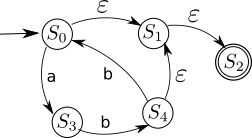
\includegraphics[width=0.4\textwidth]{img_11_3.png}
\caption{Diagrama de Transición} \label{img_11_3}
\end{figure}
$I=\{a,b\}$
$F=\{s_2\}$
Obtener:
\begin{itemize}
\item $\mbox{clausura}_\varepsilon(s_3) \qquad d(s_0,a)$
\item $\mbox{clausura}_\varepsilon(s_0) \qquad d(s_0,b)$
\item $\mbox{clausura}_\varepsilon(s_4) \qquad d(\{s_3,s_4\},b)$
\end{itemize}

\textbf{Solución: }
\begin{align*}
\mbox{clausura}_\varepsilon(s_3)	&=\{s_3\}	\\
\mbox{clausura}_\varepsilon(s_0)	&=\{s_0,s_1,s_2\}	\\
\mbox{clausura}_\varepsilon(s_4)	&=\{s_4,s_1,s_2\}	\\
d(s_0,a)	&=\{s_3\}	\\
d(s_0,b)	&=\phi	\\
d(\{s_3,s_4\},b)	&=d(s_3,b)\cup d(s_4,b)=\{s_4,s_0\}
\end{align*}
\chapter{Repaso}
\section{AFD - Función de transición extendida}
Sea un AFD $D=(S,I,\delta,s^*,F)$, la función de transición extendida:
$$\widehat{\delta}:S\times I^*\rightarrow S$$
Queda definida:
\begin{itemize}
\item $\widehat{\delta}(s,\varepsilon)=s\qquad \forall s\in S$
\item $\widehat{\delta}(s,au)=\widehat{\delta}(\delta(s,a),u)\qquad a\in I,u\in I^*, s\in S$
\end{itemize}
\section{AFND - Función de transición extendida}
Sea un AFND $N=(S,I,\delta,s^*,F)$ la función de transición extendida $\widehat{\delta}$:
$$\widehat{\delta}:P(s)\times I^*\rightarrow P(s)$$
\begin{itemize}
\item $\widehat{\delta}(\phi,w)=\phi	\qquad w\in I^*$
\item $\widehat{\delta}(A,\varepsilon)=A	\qquad A\subseteq S$
\item $\widehat{\delta}(A,au)=\widehat{\delta}(\bigcup_{s\in A}\delta(s,a),u)\qquad a\in I, A\subseteq S, s\in A, u\in I^*$
\end{itemize}
\section{Equivalencia entre AFND y AFD}
Para cualquier AFND se puede construir un AFD que reconozca el mismo lenguaje, sea el AFND $N=(S,I,\delta,s^*,F)$. El AFD equivalente será $D=(S^d,I,\delta^d,s^{*d},F^d)$ en la que:

$S^d=P(S)$, donde:
\begin{itemize}
\item Para cada $X\subseteq S \land a\in I$
$$\delta^d(X,a)=\bigcup_{s\in X}\delta^d(s,a)$$
\item Para cada $a\in I, \quad \delta^d(\phi,a)=\phi$
\item $F^d=\{X\subseteq S/X\cap F\not=\phi\}$
\end{itemize}
Utilizamos el siguiente lema para probar la equivalencia.

\textbf{Lema: }Sea $D$ y $N$ los autómatas definidos anteriormente. Entonces para cada $X\subseteq S$ y $w\in I^*$
$$\widehat{\delta}^d(X,w)=\widehat{\delta}(X,w)$$

\textbf{Prueba: }Usaremos inducción sobre \textbar w\textbar. Para $w=\varepsilon$ tiene $\widehat{\delta}^d(X,\varepsilon)=\downlegend{X}{(1)}=\widehat{\delta}(X,\varepsilon)$

(1): por concepto de AFD.

Por hipótesis de inducción, para una cadena de longitud $n, w$ se cumple:
$$\widehat{\delta}^d(X,w)=\widehat{\delta}(X,w)$$

Bastará probar que $\widehat{\delta}^d(X,aw)=\widehat{\delta}(X,aw)$

\textbf{CASO I: }$X=\phi$
\begin{align*}
\widehat{\delta}^d(\phi,aw)	&=\widehat{\delta}^d(\delta^d(\phi,a),w)	\\
			&=\widehat{\delta}^d(\phi,w)\stackrel{hi}{=}\widehat{\delta}(\phi,w)	\\
			&=\phi	\\
			&\stackrel{AFND(a)}{=}\widehat{\delta}(\phi,aw)
\end{align*}

\textbf{CASO II: }$X\not=\phi$
\begin{align*}
\widehat{\delta}(X,aw) &\stackrel{b.AFD}{=}\widehat{\delta}^d(\delta^d(X,a),w)	\\
		&=\widehat{\delta}^d\left(\underbrace{\bigcup_{s\in X}\delta^d(s,a)}_{B},w\right)	\\
		&\mbox{por la construcción}	\\
		&=\widehat{\delta}^d(B,w)	\\
		&=\widehat{\delta}(B,w)	\\
		&=\widehat{\delta}\left(\bigcup_{s\in X}\delta^d(s,a),w\right)	\\
		&=\widehat{\delta}(X,aw)
\end{align*}

\textbf{Teorema: }Sea $N=(S,I,\delta,s^*,F)$ un AFND, entonces existe un AFD $D=(S^d,I,\delta^d,s^{*d},F^d)$ que es equivalente a $N$.

\textbf{Prueba: }Sea $N$ un AFND $N=(S,I,\delta,s^*,F)$ y un AFD $D=(P(S),I,\delta^d,s^{*d},F^d)$ donde $\delta^d$ y $F^d$ siguen las definiciones anteriores.

Para probar que $L(D)=L(N)$ basta probar que :
$$w\in L(D) \Leftrightarrow w\in L(N)\quad \forall w\in I^*$$

Tomemos una cadena $w\in I^*$ arbitraria, se cumple:
\begin{align*}
w\in L(D)&\Leftrightarrow \widehat{\delta}^d(s^*,w) \in F^d	\\
		&\Leftrightarrow \widehat{\delta}^d(s^*,w)\cap F^d\not=\phi	\\
		&\Leftrightarrow \widehat{\delta}(s^*,w)\cap F^d\not=\phi	\\
		&\Leftrightarrow w\in L(N)
\end{align*}

\textbf{Ejemplo: }Sea el AFND $N$ sobre $I=\{a,b\}$ dado por el D.T:
%figura 12.1
\begin{figure}[h!]
\centering
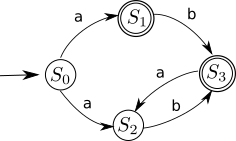
\includegraphics[width=0.4\textwidth]{img_12_1.png}
\caption{Diagrama de Transición}\label{img_12_1}
\end{figure}
Obtener el AFD $D$ equivalente.

\textbf{Solución: }Para $N: S=\{s_0,s_1,s_2,s_3\}, F=\{s_1,s_3\}, s^*=s_0$

La tabla de transición de N:
\begin{center}
\begin{tabular}{c|cc}
	&\multicolumn{2}{c}{$\delta$}	\\
	&a	&b	\\ \hline
$\phi$	&$\phi$	&$\phi$	\\
$\rightarrow s_0$ &$\{s_1,s_2\}$	&$\phi$	\\
\#$s_1$	&$\phi$	&$s_3$	\\
$s_2$	&$\phi$	&$s_3$	\\
\#$s_3$	&$s_2$	&$\phi$
\end{tabular}
\end{center}
\begin{align*}
A=\{s_1,s_2\}	\\
\delta(s_1,d)\cup\delta(s_2,d)	\\
I=\{a,b\}
\end{align*}
\begin{center}
\begin{tabular}{c|cc}
	&a	&b	\\ \hline
$\{s_0\}$	&$\{s_1,s_2\}\checkmark$	&$\phi\checkmark$	\\
$\{s_1,s_2\}$	&$\phi$	&$\{s_3\}\checkmark$	\\
$\phi$	&$\phi$	&$\phi$	\\
$\{s_3\}$	&$\{s_2\}$	&$\phi$	\\
$\{s_2\}$	&$\{\phi\}$	&$\{s_3\}$
\end{tabular}
\end{center}
%grafico 12.2
\begin{figure}[h!]
\centering
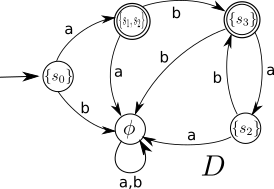
\includegraphics[width=0.5\textwidth]{img_12_2.png}
\caption{Diagrama de Transición}\label{img_12_2}
\end{figure}

\section{Conversión de un AFND -$\varepsilon$ a un AFD}
Definiremos operaciones básicas que describen computaciones en los estados de un AFND.
\begin{center}
\begin{tabular}{c|p{8cm}}
Operación	&Descripción	\\ \hline
$clausura_\varepsilon(s)$	&Conjunto de estados alcanzables desde $s$ usando solo transiciones $\varepsilon$.	\\
$clausura_\varepsilon(Q)$	&$\bigcup_{q\in Q}clausura_\varepsilon(q)$	\\
$mover(Q,a)$	&Conjuntos de estados del AFND, en los cuales hay una transición al leer el símbolo $a$ desde algún estado $q\in Q$.
\end{tabular}
\end{center}

\section{Técnica de Construcción de Subconjuntos}

\textbf{Entrada: }Un AFND $N=(S,I,\delta,s^*,F)$

\textbf{Salida: }Un AFD $D$ que acepta el mismo lenguaje $D=(S^d,I,\delta^d,s^{*d},F^d)$\\

El estado inicial de $D$ es $s^{*d}=clausura_\varepsilon(s^*)$.\\

$D_{tran}$, es la tabla de transición para $D$. $F^d$, son los estados de aceptación de $D$, son todos aquellos estados de $N$ que incluyen al menos un estado de aceptación de $N$.\\

El conjunto de estados de $D$, se denotará por $D_{estados}$.

Inicialmente, $clausura_\varepsilon(s^*)$ es el único estado de $D_{estados}$ y está sin marcar.\\
\\

\begin{algorithm}

\While {Exista un estado sin marcar Q en $D_{estados}$}{
	\For {cada símbolo de entrada} {
		$U=clausura_\varepsilon(mover(Q,a))$\\
		\If {U no esta en $D_{estados}$}{
			añadir U como un estado no marcado a $D_{estados}$		
		}
		$D_{tran}(Q,a)=U$	
	}
}
\end{algorithm}

Sea el AFND-$\varepsilon$ $N$ sobre $I=\{a,b\}$ convertido a un AFD $D$.
%grafico 12.3
\begin{figure}[h!]
\centering
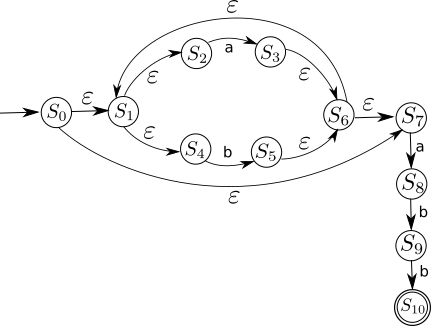
\includegraphics[width=0.65\textwidth]{img_12_3.png}
\caption{Diagrama de Transición}\label{img_12_3}
\end{figure}

Se tiene $F=\{s_{10}\}, s^*=s_0$. Hallamos $s^{*d}=clausura_\varepsilon(s_0)=\{s_0,s_1,s_2,s_4,s_7\}=A$ (sin marcar).

\begin{enumerate}
\item Marcamos $A$ y calcular:
	\begin{itemize}
	\item $D_{tran} (A,a)=clausura_\varepsilon(mover(A,a))$
	\begin{align*}
mover(A,a)=\{s_3,s_8\}	&	\\
\delta(s_0,a)=\phi \qquad &\delta(s_2,a)=s_3	\\
\delta(s_1,a)=\phi 	\qquad &\delta(s_4,a)=\phi	\\
							&\delta(s_7,a)=s_8	\\
	\end{align*}
	\begin{align*}
clausura_\varepsilon(\{s_3,s_8\})&=clausura_\varepsilon(s_3)\cup clausura_\varepsilon(s_8)	\\
				&=\{s_3,s_6,s_7,s_1,s_2,s_4\}\cup \{s_8\}	\\
				&=\{s_6,s_7,s_1,s_2,s_3,s_4,s_8\}\not = A
	\end{align*}
	Por eso lo llamaremos $B$(no marcado).

	\item $D_{tran}(A,B)=clausura_\varepsilon(mover(A,b))$
	\begin{align*}
mover(A,b)&=\{s_5\}	\\
\delta(s_4,b)	&=s_5	\\
clausura_\varepsilon(\{s_5\})&=\{s_5,s_6,s_7,s_1,s_2,s_4\}=C (no\; marcado)
	\end{align*}
	\end{itemize}
\item Marcamos $B$ y calcular.
	\begin{itemize}
	\item $D_{tran}(B,a)=clausura_\varepsilon(mover(B,a))$. Vemos el conjunto B.
	$$mover(B,a)=\{s_3,s_8\}$$
	\begin{align*}
	clausura_\varepsilon(\{s_5,s_9\})&=clausura_\varepsilon(\{s_5\})\cup clausura_\varepsilon(\{s_9\})	\\
	ignorar:	&=\{s_5,s_6,s_7,s_1,s_2,s_4,s_9\}=D (es \not= de\; B)\\
	clausura_\varepsilon(\{s_3,s_8\})	&=B(\mbox{ya lo teniamos})
	\end{align*}
	\item $D_{tran}(B,b)=clausura_\varepsilon(mover(B,b))$
	\begin{align*}
	mover(B,b)	&=\{s_5,s_9\}	\\
			&=clausura_\varepsilon(\{s_5,s_9\}=clausura_\varepsilon(\{s_5\})\cup clausura_\varepsilon(\{s_9\})	\\
			&=\{s_1,s_2,s_4,s_5,s_6,s_7,s_9\}	\\
			&=D
	\end{align*}
	\end{itemize}
\item Marcamos $C$ y calcular:
	\begin{itemize}
	\item $D_{tran}(C,a)=clausura_\varepsilon(mover(C,a))$
	\begin{align*}
	mover(C,a)	&=\{s_3,s_8\}	\\
				&=clausura_\varepsilon(\{s_3,s_8\})	\\
				&=B
	\end{align*}
	\item $D_{tran}(C,b)=clausura_\varepsilon(mover(C,b))$
	\begin{align*}
	mover(C,b)	&=\{s_5\}	\\
				&=clausura_\varepsilon(\{s_5\})=C
	\end{align*}
	\end{itemize}
\item Marcamos $D$ y calcular:
	\begin{itemize}
	\item $D_{tran}(D,a)=clausura_\varepsilon(mover(D,a))$
	\begin{align*}
	mover(D,a)	&=\{s_3,s_8\}	\\
				&=clausura_\varepsilon(\{s_3,s_8\})=B
	\end{align*}
	\item $D_{tran}(D,b)=clausura_\varepsilon(mover(D,b))$
	\begin{align*}
	mover(D,b)	&=\{s_5,s_{10}\}	\\
				&=clausura_\varepsilon(\{s_5,s_{10}\})	\\
				&=clausura_\varepsilon(\{s_5\})\cup clausura_\varepsilon(\{s_{10}\})	\\
	clausura_\varepsilon(\{s_{10}\})=\{s_{10}\}	\\
				&=clausura_\varepsilon(\{s_5,s_{10}\})	\\
				&=\{s_1,s_2,s_4,s_5,s_6,s_7,s_{10}\}=E	(s_{10}\in E)
	\end{align*}
	\end{itemize}
\item Marcamos $E$ y calcular:
	\begin{itemize}
	\item $D_{tran}(E,a)=clausura_\varepsilon(mover(E,a))$
	\begin{align*}
	mover(E,a)	&=\{s_3,s_8\}	\\
				&=clausura_\varepsilon(\{s_3,s_8\})=B	\\
	\end{align*}
	\item $D_{tran}(E,b)=clausura_\varepsilon(mover(E,b))$
	\begin{align*}
	mover(E,b)	&=\{s_5\}	\\
				&=clausura_\varepsilon(\{s_5\})=C
	\end{align*}
	\begin{center}
	\begin{tabular}{c|cc}
		&a	&b	\\ \hline
	A	&B	&C	\\
	B	&B	&D	\\
	C	&B	&C	\\
	D	&B	&E	\\
	E	&B	&C	
	\end{tabular}
	\end{center}
	%grafico 12.4
	\begin{figure}[h!]
	\centering
	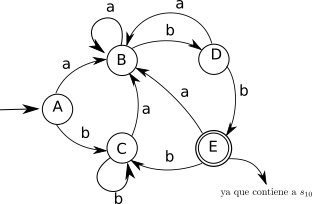
\includegraphics[width=0.5\textwidth]{img_12_4.png}
	\caption{Diagrama de Transición}\label{img_12_4}
	\end{figure}
	\end{itemize}
\end{enumerate}
\chapter{Gramáticas}

Mientras que los autómatas nos sirven para reconocer cadenas de un lenguaje, las gramáticas son un formalismo diseñado para la definición de lenguajes. Representan un medio para la generación de cadenas que pertenecen a un lenguaje. El elemento fundamental en una gramática es la regla.

\section{Regla}

Dado un alfabeto $\Sigma$, una regla(o producción) definida sobre $\Sigma$, es un par ordenado $(x,y)$ donde $x,y\in \Sigma^*$. Aquí se dirá a:
\begin{itemize}
\item x: Parte izquierda de la regla.
\item y: Parte derecha de la regla.
\end{itemize}

\textbf{Notación: }$x::=y$

\subsection{Regla Compresora}
Una regla es compresora cuando la longitud de la parte izquierda es mayor o igual a la longitud de la parte derecha.

$$
|x|\geq |y|
$$

\section{Tipos de Derivación}
\subsection{Derivación Directa}
Dado un alfabeto $\Sigma$, un conjunto de producciones $P$ sobre $\Sigma$, donde:

$P= \left \{ \begin{array}{c}
					x_1::=y_1\\
					x_2::=y_2\\
					\vdots \\
					x_n::=y_n \end{array} \right.$
					

y sea $v,w\in \Sigma^*$. Diremos que $w$ deriva directamente de $v$, si $\exists t,u \in \Sigma^*$ y una regla en $P$; $x_i::=y_i$. tal que $v=tx_iu$  y  $w=ty_iu$

\textbf{Notación: } $v\rightarrow w$; se lee ''$v$ produce directamente $w$''.

\textbf{Definición: } Dado un alfabeto $\Sigma$, un conjunto de producciones sobre $\Sigma$ y $v,w\in\Sigma^*$, se dice que $w$ deriva de $v$ si $\exists w_0,w_1,...w_m \in\Sigma^*$ tales que:
\begin{align*}
v	=&w_0\rightarrow w_1\\
	 & w_1\rightarrow w_2\\
	 &\vdots\\
	 &w_{m-1}\rightarrow w_m = w 
\end{align*}

\textbf{Notación: }$v\xrightarrow{*}w$ se lee $v$ produce $w$.

\textbf{Ejemplo: }Defina un conjunto de reglas que permitan la correcta formación de frases.

\textbf{Solución: }Sea el conjunto de producciones $P$:
\begin{align*}
\begin{array}{lrl}
	R_1	&	<oracion>&::=<sujeto><predicado>	\\
	R_2	&	<sujeto>&::=<articulo><sustantivo>	\\
	R_3	&	<predicado>&::=<verbo><complemento>	\\
	R_4	&	<predicado>&::=<verbo>	\\
	R_5	&	<articulo>&::=el	\\
	R_6	&	<articulo>&::=la	\\
	R_7	&	<sustantivo>&::=atleta	\\
	R_8	&	<sustantivo>&::=voleibolista	\\
	R_9	&	<verbo>&::=salta	\\
	R_{10}&	<verbo>&::=corre	\\
	R_{11}&	<complemento>&::=alto	\\
	R_{12}&	<complemento>&::=velozmente
\end{array}
\end{align*}

A partir de $P$ y comenzando en el item $<oracion>$ podemos obtener:
\begin{center}
	''el atleta salta alto''\\
	''la voleibolista corre velozmente''\\
	''la voleibolista salta''
\end{center}
Pero hay frases que no podríamos generar como: ''velozmente salta voleibolista''.

\textbf{Ejemplo: }Describa como se construye la frase ''la voleibolista salta'' a partir de $<oracion>$

\textbf{Solución: }
\begin{align*}
<oracion>&\rightarrow<sujeto><predicado>	& (R_1)	\\
		 &\xrightarrow{*}<articulo><sustantivo><predicado>	& (R_2)	\\
		 &\xrightarrow{*}<articulo><sustantivo><verbo>	& (R_4)	\\
		 &\xrightarrow{*}la <sustantivo><verbo>			& (R_6)	\\
		 &\xrightarrow{*}\mbox{la voleibolista }<verbo>	& (R_8)	\\
		 &\xrightarrow{*}\mbox{la voleibolista salta}	& (R_9)	
\end{align*}
\textbf{Ejemplo: }Defina un conjunto de reglas que describan cómo son las  las instrucciones que permiten asignar el valor de una expresión a una variable en un lenguaje de programación.'m'

\textbf{Solución: }Sea el conjunto $P$.
\begin{align*}
\begin{array}{lrl}
R_1	&	<asignacion>&::=<variable>'=\,'<expresion>	\\
R_2	&	<expresion>&::=<variable>	\\
R_3	&	<expresion>&::=<numero>		\\
R_4	&	<expresion>&::=<expresion>'+\;'<expresion>	\\
R_5	& 	<expresion>&::=<expresion>'*\;'<expresion>	\\
R_6	&	<variable>&::='A\;'\\
R_7	&	<variable>&::='B\;'	\\
R_8	&	<variable>&::='C\;'	\\
R_9	&	<numero>&::='3\;'		\\
R_{10}&	<numero>&::='6\; '		\\
\end{array}
\end{align*}
Si asumimos que A,B,C son $<variables>$; 3, 6 son $<numeros>$ podremos generar:
%Obtenemos instrucciones como:
\begin{align*}
A&=B+C	\\
B&=B*3	\\
C&=B+6
\end{align*}
No podemos obtener las siguientes instrucciones:
\begin{align*}
A&=+2*+4	\\
4&=B
\end{align*}

En resumen:
\begin{itemize}
\item El objeto es llegar a tener una secuencia correcta de símbolos.
\item Los símbolos son: el, la, atleta, voleibolista, corre, etc. A, B, C, 3, 6, *, +
\item Se usan algunas producciones.
\end{itemize}

\textbf{Definición: }Una gramática formal definida sobre $\Sigma$ es una cuádrupla $G=(\Sigma_N,\Sigma_T,P,s)$ donde:
\begin{align*}
\Sigma_N	&: \mbox{Alfabeto de símbolos no terminales}	\\
\Sigma_T	&: \mbox{Alfabeto de símbolos terminales}	\\
P			&: \mbox{Conjunto de producciones}	\\
s			&: \mbox{símbolo inicial}	\\
\end{align*}
Además se cumple:
\begin{itemize}
\item $s\in \Sigma_N$
\item $\Sigma_N \cap \Sigma_T=\phi$
\item $\Sigma=\Sigma_N\cup\Sigma_T$
\end{itemize}
\textbf{Ejemplo: }Defina formalmente una gramática para obtener cualquier número natural precedido de un signo.

\textbf{Solución: }Los elementos de $G$ son:
\begin{align*}
\Sigma_T	&=\{+,-,0,1,...,9\}	\\
\Sigma_N	&=\{<signo>,<digito>,<numero>,<caracter>\}	\\
s			&=<numero>	\\
\end{align*}
\begin{align*}
P\left \{ \begin{array}{rl}
<numero>	&::=<signo><digito>	\\  
<signo>		&::= +	\\
<signo>		&::= -	\\
<digito>	&::= <caracter><digito>	\\
<digito>	&::= <caracter>	\\
<caracter>	&::= 0	\\
<caracter>	&::= 1	\\
			&\vdots	\\
<caracter>	&::= 9	
\end{array}\right.
\end{align*}
Con esta gramática generamos números como: $+371,-4692,+7$.

\section{Forma Normal de Backus-Naur (BNF)}
Es una forma estandarizada de enunciar la composición de una gramática. En la BNF:
\begin{itemize}
\item Los símbolos no terminales inician en ''\textless'' y terminan en ''\textgreater''.
\item La regla $(S,T)$ se expresa $S::=T$
\item Las reglas de la forma:
	$s::=T_1, s::=T_2,...,s::=T_n$

pueden combinarse en: $s::=T_1|T_2|...|T_n$. La barra se lee como ''ó''
\end{itemize}

\textbf{Ejemplo: }Defina el conjunto $P$ usando la notación BNF.
\begin{align*}
P\left\{ \begin{array}{rl}
<numero>	&::=<signo><digito>	\\	
<signo>		&::=+ | -	\\
<digito>	&::=<digito><caracter>|<caracter>	\\
<caracteer>	&::=0|1|2|...|9 
\end{array}\right.
\end{align*}

\textbf{Definición: }La relación $\xrightarrow{n}$ se define recursivamente mediante:
\begin{itemize}
\item $x\xrightarrow{0}x\qquad \forall x\in\Sigma^*$
\item $w\xrightarrow{n}xuy \cap u\rightarrow v$ entonces $w\xrightarrow{n+1}xvy;	\quad x,y,u,v,w \in\Sigma^*$

Cuando se tiene $x\xrightarrow{n}y$ se lee $y$ deriva de $x$ en $n$ pasos.
\end{itemize}

\textbf{Observación: }Se usarán las notaciones:
\begin{itemize}
\item $x\xrightarrow{*}y$ si existe $n \geq 0$ tal que $x\xrightarrow{n}y$
\item $x\xrightarrow{+}y$ si existe $n>0$ tal que $x\xrightarrow{n}y$
\end{itemize}

\textbf{Ejemplo: }Sea la gramática $G$, donde $P$ está dado por:
\begin{align*}
\begin{array}{lrl}
R_1	&s	&::=aAbc \\
R_2	&A	&::=aAbC	\\
R_3	&A	&::=\varepsilon	\\
R_4	&Cb	&::=bC	\\
R_5	&Cc	&::=cc
\end{array}
\end{align*}
Verifique:
\begin{itemize}
\item Si.\\     
$
\begin{array}{lrl}
	&s	&\xrightarrow{2}abc	\\
(R_1)& s &::=aAbc	\\
(R_3)&	 &::=abc
\end{array}
$

\item $s\xrightarrow{n}a^3b^3c^3 \qquad n=?$
\end{itemize}

\textbf{Ejemplo: }La siguiente gramática se usa para generar cualquier numero natural precedido de un signo. Los elementos para G seran:
\begin{align*}
\Sigma_T	&=\{0,1,2,...,9,+,-,(,)\}	\\
\Sigma_N	&=\{<signo>,<digito,<numero>,<caracter>\}	\\
\end{align*}
Donde S está formado por:
\begin{align*}
S\left \{\begin{array}{rl}
<numero>&::=<signo><digito>\\	
<signo>&::=+	\\
<signo>&::=-	\\
<digito>&::=<caracter><digito>	\\
<digito>&::=<caracter>	\\
<caracter>&::=0	\\
<caracter>&::=1	\\
 \vdots & \\
<caracter>&::=9	\\
\end{array}\right.
\end{align*}


\textbf{Definición:} Dada una gramática $G=(\Sigma_N,\Sigma_T,P,S)$, llamaremos lenguage generado a partir de una gramatica $G$ al conjunto:

$$
L(G)=\{w \in \Sigma_{T}^{*}/S\xrightarrow{*} w\}
$$

Son las palabras formadas por simbolos terminales derivables a partir del simbolo inicial S.

\textbf{Definición(Recursividad): }Una gramática es recursiva si tiene alguna derivación recursiva, es decir si $A\xrightarrow{*}xAy$ donde $A\in \Sigma_N, x,y\in \Sigma^*$
\begin{itemize}
\item Si $x=\varepsilon$ la gramática es recursiva por la izquierda.
\item Si $y=\varepsilon$ la gramática es recursiva por la derecha.
\end{itemize}

\textbf{Ejemplo: }Sea la gramática que genera expresiones aritméticas conteniendo operadores de suma, resta y paréntesis.
\begin{align*}
\Sigma_T	&=\{0,1,2,...,9,+,-,(,)\}	\\
\Sigma_N	&=\{E,T,N,D\}	\\
\end{align*}
donde P está formado por:
\begin{align*}
P\left \{\begin{array}{rl}
E	&::=E+T|E-T|T\\	
T	&::=(E)|N	\\
N	&::=DN|D	\\
D	&::=0|1|...|9	
\end{array}\right.
\end{align*}

Se pide:
\begin{itemize}
\item A partir de T obtenga una secuencia de sumas y/o restas de T usando recursividad a la izquierda.
\item A partir de N genere un número de 4 cifras usando recursividad a la derecha.
\end{itemize}

\textbf{Solución: }
\begin{itemize}
\item 
\begin{align*}
E	&\rightarrow E+T	\qquad &(R_1)	\\
	&\xrightarrow{*}E-T+T	&(R_2)	\\
	&\xrightarrow{*}E-T-T+T	&(R_2)	\\
	&\xrightarrow{*}T-T-T+T	&(R_3)	\\
\end{align*}
\item 
\begin{align*}
N	&\rightarrow DN		&(R_6)	\\
	&\xrightarrow{*}DDN	&(R_6)	\\
	&\xrightarrow{*}DDDN	&(R_6)	\\
	&\xrightarrow{*}DDDD	&(R_7)	\\
\end{align*}
\end{itemize}

\section{Clasificación de las Gramáticas}

\subsection{Gramáticas Regulares (GR)}
Se llaman también lineales y es el grupo más restringido de gramática. En la parte derecha de la regla tenemos como máximo dos símbolos.

Hay dos tipos de gramáticas regulares:
\begin{enumerate}
\item Gramática Lineal por la Derecha (GLD). Sus reglas son de la forma:

$\begin{array}{clc}
A&::=a	&\qquad A,B\in \Sigma_N \\
A&::=aB	&\qquad a\in\Sigma_T	\\
A&::=\varepsilon	&
\end{array}$
	
\item Gramática Lineal por la Izquierda (GLI). Sus reglas son de la forma:
\begin{align*}
A&::=a	\\
A&::=Ba	\\
A&::=\varepsilon
\end{align*}
\end{enumerate}
Hay una equivalencia entre la GLD y la GLI.

\textbf{Ejemplo: }Sea la gramática regular.
\begin{align*}
P\left\{\begin{array}{rl}
S&::=aA	\\	
S&::=bA	\\
A&::=bB	\\
A&::=a	\\
B&::=aA	\\
B&::=bA		
\end{array}\right.
\end{align*}
Entonces:
\begin{itemize}
\item Determine si $ba\in L(G)$
\item Muestre una derivación de la cadena $w=bababa$
\end{itemize}
\chapter{Autómatas Finitos y Gramáticas Regulares}

\textbf{Teorema: }La clase de los lenguajes generados por una gramática regular es precisamente la de los lenguajes regulares.

\section{Procedimiento de Conversión de una GR a un AF}
\begin{enumerate}
\item Para cada símbolo no terminal de la gramática asociar un estado en el autómata.
\item Para cada regla $A::=bC$ en la gramática origina una transición $(A,b,C)$ en el autómata.
\item Para cada regla $A::=b$ se tendrá transiciones $(A,b,Z)$ donde $Z$ será el único estado final del autómata.
\end{enumerate}

\textbf{Ejemplo: }Sea la GR $G=(\Sigma_N,\Sigma_T,S,P)$ donde $P$ esta dado por:
\begin{align*}
\mbox{Del ejemplo anterior: }	\\
S::=aA	\\
S::=bA	\\
A
\end{align*}
%grafico 14.1
\begin{figure}[h!]
\centering
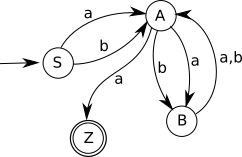
\includegraphics[width=0.4\textwidth]{img_14_1.png}
\caption{Diagrama de Transición}\label{img_14_1}
\end{figure}

\section{Procedimiento de Conversión de un AFD a un GR}

\begin{enumerate}
\item Para cada transición de la forma $((\downlegend{p}{(1)},a),\downlegend{q}{(2)})$ en el AFD( (1): estado anterior, (2): estado siguiente), donde:

$p,q\in S, a\in I$ habrá una regla $X_p::=aX_q$ en la gramática. En la que $X_i$ es la variable en que corresponde al estado $i$ del AFD.
\item Para cada transición $((p,a),q)$ donde $q\in F$ incorpora ademas la regla.
$$X_p::=a\qquad (\mbox{también }X_p::=aX_q)$$
\end{enumerate}
\textbf{Ejemplo: }Dado el AFD. Obtener la GR equivalente.
%grafico 14.2
\begin{figure}[h!]
\centering
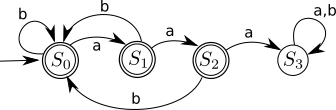
\includegraphics[width=0.4\textwidth]{img_14_2.png}
\caption{Diagrama de Transición}\label{img_14_2}
\end{figure}

\textbf{Solución: }Se obtiene las siguientes reglas:
\begin{align*}
P\left \{ \begin{array}{c}
s_0::=bs_0	\\
s_0::=as_1	\\
s_1::=as_2	\\
s_1::=bs_0	\\
s_2::=as_3	\\
s_2::=as_0	\\
s_3::=as_3	\\
s_3::=bs_3	\\
s_0::=b	\\
s_0::=a	\\
s_1::=a	\\
s_1::=b	\\
s_2::=b
\end{array}\right.
\end{align*}
Dado un AFD $D=(S,I,\delta,s^*,F)$ se desea encontrar un GLD $G$, tal que $L(D)=L(G)$. Si $q$ no es un estado final, la gramática buscada es $G=(\Sigma_N,\Sigma_T,P,q)$ en la que $P$ consiste de reglas de la forma: 
\begin{align*}
p&::=aq	&\mbox{Si }\delta(p,a)=q	\\
p&::=a	&\mbox{Si }\delta(p,a)=q\in F
\end{align*}
\textbf{Ejemplo: }Sea el AFD $D$ dado por Fig \ref{img_14_3}:
%grafico 14.3
\begin{figure}[h!]
\centering
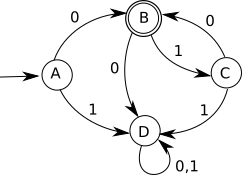
\includegraphics[width=0.4\textwidth]{img_14_3.png}
\caption{Diagrama de Transición}\label{img_14_3}
\end{figure}
\begin{align*}
A&::=0B	\\
A&::=1D\qquad\xmark	\\
B&::=0D\qquad\xmark	\\
B&::=1C	\\
C&::=0B	\\
C&::=1D\qquad\xmark	\\
D&::=0D\qquad\xmark	\\
D&::=1D\qquad\xmark	\\
A&::=0	\\
C&::=0
\end{align*}
$D$ es un estado muerto, quitamos las reglas de la forma $p::aD$

Quedará:
\begin{align*}
P\left \{ \begin{array}{c}
A::=0B	\\
B::=1C	\\
C::=0B	\\
A::=0	\\
C::=0
\end{array}\right.
\end{align*}
$0$ y $1$ son $\Sigma_T$

\section{Conversión de una Gramática Regular GR a AFND-$\varepsilon$}
Sea la GLD $G=(\Sigma_N,\Sigma_T,s,P)$ encontraremos un AFND-$\varepsilon$.
$$N=(S^{nd},I^{nd},\delta^{nd},s^*,F^{nd})$$
tal que $L(G)=L(N)$

Sea:
\begin{enumerate}
\item $I^{nd}=\Sigma_T$
\item Los estados $S^{nd}$ de $N$ serán $S$ además de los sufijos de la parte derecha de las reglas.
\item $s^*=S$
\item Para definir $\delta$, se tiene:
	\begin{itemize}
	\item Si $\alpha::=\beta\quad\in P$ entonces se define $\delta(\alpha,\varepsilon)=\beta$
	\item Si $a\alpha\in S^{nd},a\in I^{nd}$ se hace $\delta(a\alpha,a)=\alpha$
	\end{itemize}
\end{enumerate}
Los estados finales $F^{nd}$ del autómata $N$ serán los estados rotulados como $\varepsilon$.

\textbf{Ejemplo: }Sea $G$ la GLD definida por:
\begin{align*}
\Sigma_T&=\{0,1\}	\\
S&::=0A	\\
A&::=|A|\varepsilon
\end{align*}
Obtener el AF equivalente.

\textbf{Solución: }
\begin{itemize}
\item $I^{nd}=\{0,1\}\cup\{\varepsilon\}$
\item $S^{nd}=\{S,0A,1A,\uplegend{A}{sufijo},\varepsilon\}$
\item $s^*=S$
\item Diagrama en Fig \ref{img_14_4}.
%grafico 14.4
\begin{figure}[h!]
\centering
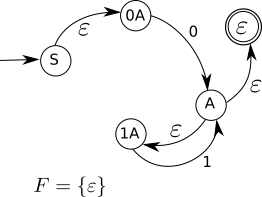
\includegraphics[width=0.4\textwidth]{img_14_4.png}
\caption{Diagrama de Transición}\label{img_14_4}
\end{figure}

\end{itemize}
\section{Jerarquía de las Gramáticas}
De acuerdo a Noam Chomsky se tiene la siguiente clasificación para las gramáticas.
\begin{enumerate}
\item G. Regulares.
\item G. Sensibles al contexto.
\item G. sin Restricciones.
\item G. Libres de contexto.
\end{enumerate}
\section{Gramáticas Sensibles al Contexto}
También se les conoce como gramáticas del tipo I y sus producciones son de la forma.
\begin{align*}
&xAy\rightarrow xvy&\\
A\in\Sigma_N,&\quad x,y\in\Sigma^*,&\quad v\in\Sigma^*
\end{align*}
En una gramática S. Contexto no hay reglas compresoras.

\textbf{Ejemplo: }Sea G la gramática.
\begin{align*}
S::=&\overbrace{abc}^{R_1}|\overbrace{aAbc}^{R_2}	\\
A::=&\overbrace{abc}^{R_3}|\overbrace{aAbc}^{R_4}	\\
Cb::=&\overbrace{bC}^{R_5}	\\
Cc::=&\overbrace{cc}^{R_6}
\end{align*}

\begin{align*}
S	&::=aAbc	&(R_2)	\\
	&::=aabCbc	&(R_3)	\\
	&::=aabbCc	&(R_5)	\\
	&::=aabbccc	&(R_6)	\\
\end{align*}

$L(G)=\{abc,\overbrace{aa}^{a^2}\overbrace{bb}^{b^2}\overbrace{ccc}^{c^3}, a^3b^3c^3,...\}$

$L(G)=\{a^nb^nc^n/n\geq 1\}$

\section{G. Sin Restricciones}
Se llaman también recursivamente enumeradas o gramáticas del tipo ''O''. Sus reglas son de la forma:

$xAy::=v\qquad A\in\Sigma_N;x,y,v\in\Sigma^*	$

\textbf{Ejemplo: }La gramática G:
\begin{align*}
\left \{ \begin{array}{c}
aS::=bSb	\\
aSb::=\varepsilon	\\
SbS::=bcS
\end{array}\right.
\end{align*}
Es una gramática sin restricciones.

\section{G. Libres de Contexto}
También conocidos como gramáticas del tipo 2. Se caracterizan porque la parte izquierda de la regla está formado por un único símbolo no terminal.
$$A::=v;	\qquad A\in\Sigma_N; \qquad v\in\Sigma^*=\Sigma_N\cup\Sigma_T;\cup:  combinacion$$

Estas gramáticas son especialmente adecuadas para representar los aspectos sintácticos de un lenguaje de programación. Se observa de la definición que podemos incluir $A\rightarrow\varepsilon$.

\textbf{Ejemplo: }
\begin{enumerate}
\item Sea $\Sigma_T=\{a,b\}$ y $P$.
\begin{align*}
S::=\overbrace{\varepsilon}^{R_1}|\overbrace{aSb}^{R_2}	\\
S::=aSb\qquad(R_2)	\\
S::aaSbb\qquad(R_2)	\\
S::=aaaSbbb\qquad(R_2)	\\
S::=a^nSb^n\qquad(R_2)	\\
S::=a^n\varepsilon b^n=a^nb^n\qquad(R_1)	\\
L(G)=\{a^nb^n/n\geq 0\}	\\
\mbox{ya que }	\\
S::=\varepsilon	\\
S\rightarrow\varepsilon
\end{align*}
\item Sea $\Sigma_T=\{a,b\}$ y $P$.
$$S::=\underbrace{aSa}_{R_1}|\underbrace{bSb}_{R_2}|\underbrace{a}_{R_3}|\underbrace{a}_{R_4}|\underbrace{\varepsilon}_{R_5}$$
\begin{align*}
L=\{a,b,\varepsilon,abaaaaba,...\}	\\
S::=aba\qquad(R_1)	\\
S::=abSba\qquad(R_2)	\\
S::=abaSaba\qquad(R_1)	\\
S::=abaaSaaba\qquad(R_2)	\\
S::=abaa|aaba\qquad(R_5)	\\
L=\{uu^R/u\in\Sigma^*\}	\\
L=\{w/w=w^R,w\in\Sigma^*\}
\end{align*}
\item Sea $\Sigma=\{a,b\}$ y $P$ dado por:
\begin{align*}
S::=aS|aB	\\
B::=bC	\\
B::=bC	\\
c::=aC|a
\end{align*}
\end{enumerate}
\chapter{Árbol de Derivación}
\textbf{Definición: }Sea $G=\{\Sigma_N,\Sigma_T,S,P\}$ una gramática libre de contexto(GLC). Un AD es un árbol ordenado, construido recursivamente como sigue:
\begin{enumerate}
\item Un árbol sin aristas cuyo único vértice tiene etiqueta $S$, es un AD de $S$.
\item Si $x\in \Sigma_N$ es etiqueta de una hoja $h$ de un AD $A$, entonces:
	\begin{itemize}
	\item Si $x\rightarrow \varepsilon \in P$, entonces el árbol obtenido incrementando a $A$ un vértice $v$ con etiqueta $\varepsilon$ y una arista $\{h,v\}$ es un AD.
	\item Si $x\rightarrow x_1x_2...x_n \in P$, donde $x_1,x_2,...x_n \in \Sigma_T \cup \Sigma_N$, entonces el árbol obtenido incrementando a $A$ $n$ vértices $v_1,v_2,...,v_n$ con etiquetas $x_1,x_2,...,x_n$ en ese orden, y con $n$ aristas $\{h,v_1\},\{h,v_2\},...\{h,v_n\}$ es un AD. 
	\end{itemize}
\end{enumerate}

\textbf{Ejemplo: }Sea $G$ un GLC donde $P$ está dado por:
\begin{align*}
& E\rightarrow E+T|T	\\
& T\rightarrow T+F|F	\\
& F\rightarrow (E)|t
\end{align*}
Obtener el AD para la cadena $w=t+(t+t)$, partiendo de E.

\textbf{Solución: }
\begin{align*}
E	&\rightarrow T			&\qquad (R_2)\\
	&\rightarrow T+F		&\qquad (R_3)\\
	&\rightarrow T+(E)		&\qquad (R_5)\\
	&\rightarrow T+(E+T)	&\qquad (R_1)\\
	&\rightarrow T+(T+T)	&\qquad (R_2)\\
\intertext{Luego se aplica las reglas reiteradas veces, uno a la vez}
	&\rightarrow F+(T+T)	&\qquad (R_4)\\
	&\rightarrow F+(F+T)	&\qquad (R_4)\\
	&\rightarrow F+(F+F)	&\qquad (R_4)\\
	&\rightarrow t+(F+F)	&\qquad (R_6)\\
	&\rightarrow t+(t+F)	&\qquad (R_6)\\
	&\rightarrow t+(t+t)	&\qquad (R_6)
\end{align*}
%GRAFICO 1
\begin{figure}[h!]
\centering
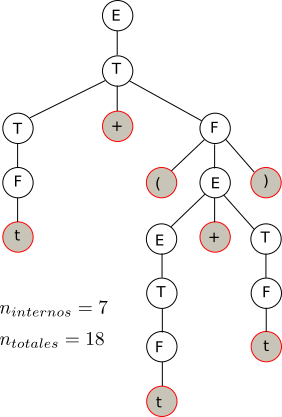
\includegraphics[width=0.3\textwidth]{img_15_1.png}
\caption{Arbol de derivación}\label{img_15_1}
\end{figure}
Se ha requerido 11 pasos para derivar $w$ (Fig \ref{img_15_1}).


\textbf{Reglas}

\begin{enumerate}
    \item La raiz se etiqueta con el simbolo inicial
    \item Los hijos de la raiz son aquellos simbolos que aparecen al lado derecho de la composicion usado para reemplazar el simbolo inicial.
    \item Todo nodo etiquetado con un no terminal tiene unos nodos hijos etiquetados en los simbolos del lado derecho de la produccion usada para sustituir ese no terminal.
    \item Los nodos que no tienene hijos deben ser etiquetados con sumbolos terminales.
\end{enumerate}


\textbf{Ejemplo: }Dada la la GLC dada por:
  \[
    P=\left\{
                \begin{array}{lll}
                    S	&\rightarrow AB		& \\
                    A	&\rightarrow aA|a	& \\
                    B	&\rightarrow bB|b	& \\
                \end{array}
              \right.
  \]
\begin{align*}
\intertext{1. Verifique si w=aabbb se deriva a partir de S}
\intertext{2. En caso afirmativo, presente el arbol de derivacion}
\intertext{\textbf{Solución: }}
S	&\rightarrow AB		&(R_1)	\\
	&\rightarrow aAB	&(R_2)	\\
	&\rightarrow aaB	&(R_3)	\\
	&\rightarrow aabB	&(R_4)	\\
	&\rightarrow aabbB	&(R_4)	\\
	&\rightarrow aabbb	&(R_5)	\\
\end{align*}
La cantidad de pesos para derviar $w$ es 6.
%graficon

Cada nodo interno del árbol será un símbolo no terminal, mientras que las hojas serán los símbolos terminales. Una regla $A:= x_1...x_n$ se representará como un símbolo cuyo nodo padre es A, siendo sus nodos hijos $x_1,x_2,...,x_n$.

\textbf{Ejemplo: }Sea $G$ la GLC dada por:
\begin{align*}
S	&\rightarrow AB		& \\
	&\rightarrow aA|a	& \\
	&\rightarrow bB|b	& \\
\intertext{Obtener el Árbol de Derivación para $w=aabbb$ e indicar la cantidad de pasos}
\intertext{\textbf{Solución: }}
S	&\rightarrow AB		&(R_1)	\\
	&\rightarrow aAB	&(R_2)	\\
	&\rightarrow aaB	&(R_3)	\\
	&\rightarrow aabB	&(R_4)	\\
	&\rightarrow aabb	&(R_5)	\\
\end{align*}
%GRAFICO 2

\begin{figure}[h!]
\centering
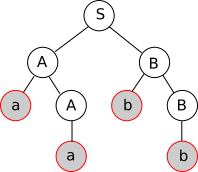
\includegraphics[width=0.22\textwidth]{img_15_2.png}
\caption{Arbol de derivación}\label{img_15_2}
\end{figure}
\begin{align*}
\left. \begin{array}{c}
n_i=4	\\
n_T=9
\end{array}\right \} \mbox{Pasos }=9-4=5 \quad \cmark
\end{align*}
\textbf{Definición: }Una GLC $G$ se llama ambigua, cuando es posible obtener dos o mas ADs diferentes para alguna sentencia que genere. Puede haber otras gramáticas GLC equivalente a una GLC ambigua, y que éstas gramáticas no sean ambiguas.

\textbf{Ejemplo: }Sea $G$ una GLC donde P esta dado por:
\begin{align*}
S	&\rightarrow S+S	&(R_1)	\\
	&\rightarrow S*S	&(R_2)	\\
	&\rightarrow (S)	&(R_3)	\\
	&\rightarrow t		&(R_4)	\\
\intertext{Obtener el AD para $w=t+t+t$ partiendo de $S$.}
\end{align*}
\textbf{Solución: }
\begin{align*}
S	&\rightarrow S+S	&(R_1)	\\
S	&\rightarrow S+S+S	&(R_1)	\\
S	&\rightarrow t+S+S	&(R_4)	\\
S	&\rightarrow t+t+S	&(R_4)	\\
S	&\rightarrow t+t+t	&(R_4)
\end{align*}
\begin{enumerate}
\item $n_i=5$, $n_t=10$.
%GRAFICO 3 
\begin{figure}[h!]
\centering
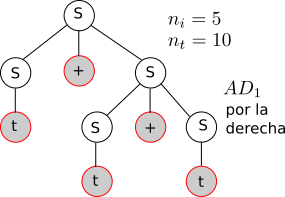
\includegraphics[width=0.3\textwidth]{img_15_3.png}
\caption{Arbol de derivación}\label{img_15_3}
\end{figure}
\item 
\begin{align*}
S	&\rightarrow S+S	&(R_1)	\\
S	&\rightarrow t+S	&(R_4)	\\
S	&\rightarrow t+S+S	&\mbox{ERROR }(R_1)	\\
S	&\rightarrow t+t+S	&(R_4)	\\
S	&\rightarrow t+t+t	&(R_4)
\end{align*}
%GRAFICO 4
\begin{figure}[h!]
\centering
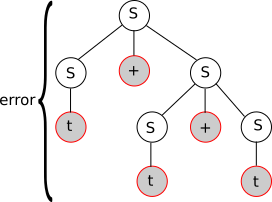
\includegraphics[width=0.45\textwidth]{img_15_4.png}
\caption{Arbol de derivación}\label{img_15_4}
\end{figure}

\begin{align*}
S	&\rightarrow S+S	&(R_1)	\\
S	&\rightarrow S+S+S	&(R_1)	\\
S	&\rightarrow S+S+t	&(R_4)	\\
S	&\rightarrow t+S+t	&(R_4)	\\
S	&\rightarrow t+t+t	&(R_4)
\end{align*}
%GRAFICO 5
\begin{figure}[h!]
\centering
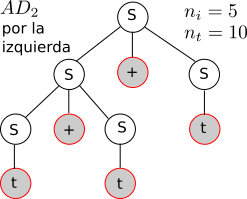
\includegraphics[width=0.45\textwidth]{img_15_5.png}
\caption{Arbol de derivación}\label{img_15_5}
\end{figure}

El (1) se puede interpretar como
$$\downlegend{t}{segundo}+(\underbrace{t+t}_{primero})$$
El (2) se puede interpretar como
$$(\underbrace{t+t}_{primero})+\downlegend{t}{segundo}$$
\end{enumerate}

\textbf{Definición: }Un lenguaje libre de contexto $L$ se dice inherentemente ambiguo si todas las GLC para $L$ son ambiguas.


\textbf{Definición: }Una derivación se denomina derivación a la izquierda si en cada paso, se expande la variable más a la izquierda.

Una derivación se dirá derivación a la derecha si en cada paso se expande la variable más a la derecha.

\textbf{Ejemplo: }Sea $G$ una GLC donde P está dado por:
\begin{align*}
S	&\rightarrow SbS	&(R_1)	\\
S	&\rightarrow ScS	&(R_2)	\\
S	&\rightarrow a		&(R_3)	\\
\end{align*}
Para la cadena $w=abaca$.
\begin{enumerate}
\item Obtener una derivación por la izquierda.
\item Obtener una derivación por la derecha.
\item Obtener su AD.
\end{enumerate}
\textbf{Solución: }
\begin{enumerate}
\item 
\begin{align*}
S	&\rightarrow \underline{S}bS	&(R_1)\\
	&\rightarrow ab\underline{S}	&(R_3)\\
	&\rightarrow ab\underline{S}cS	&(R_2)\\
	&\rightarrow abacS				&(R_3)\\
	&\rightarrow abaca				&(R_3)
\end{align*}
\item
\begin{align*}
S	&\rightarrow Sc\underline{S}	&(R_2)\\
	&\rightarrow \underline{S}ca	&(R_3)\\
	&\rightarrow Sb\underline{S}ca	&(R_1)\\
	&\rightarrow \underline{S}baca	&(R_3)\\
	&\rightarrow abaca				&(R_3)
\end{align*}
\item $\,$\\
%GRAFICO 6
\begin{figure}[h!]
\centering
\includegraphics[width=0.4\textwidth]{img_15_6.png}
\caption{Arbol de derivación}\label{img_15_6}
\end{figure}
\end{enumerate}
\section{Equivalencia en Gramáticas}
Un mismo lenguaje puede ser generado por mas de una gramática.

\textbf{Definición: }Dos gramáticas $G^1$ y $G^2$ se llaman equivalentes, si ambas generan el mismo lenguaje sobre $\Sigma_T$. Es decir:
$$L(G^1)=L(G^2)$$
Esto es, si generan el mismo lenguaje.

En muchas ocasiones es recomendable simplificar ciertas gramaticas eliminando simbolos o reglas no deseadas.

\subsubsection{Elementos Indeseables en Gramáticas}
\textbf{Definición: }Una regla innecesaria es una producción de la forma $A:=A$.

\textbf{Definición: }Sea $G=(\Sigma_N,\Sigma_T,S,P)$ una GLC. Una variable $X\in \Sigma_N$ se llama útil si y solo si existen dos cadenas $u,v\in\Sigma^*$ tales que:
\begin{align*}
S	\xrightarrow{*} uXv \mbox{ y existe } w\in{\Sigma_T}^* \mbox{ tal que } uXv\xrightarrow{*}w
\end{align*}
\textbf{Definición: }Un símbolo inaccesible o inútil es aquel símbolo no terminal que no aparece en ninguna cadena de símbolos que pueda derivarse a partir del símbolo inicial de la gramática.

\textbf{Ejemplo: }Sea $G$ la GLC dado por:
\begin{align*}
S	&\rightarrow AB|a	\\
B	&\rightarrow b	\\
C	&\rightarrow c	\\
\intertext{Identifique las variables inútiles}
\end{align*}
\textbf{Solución: }
\begin{itemize}
\item C es una variable inútil. No existen subcadenas $u,v$ tales que $S\xrightarrow{*}uCv$.
\item A es inútil?. Vemos subcadenas $u,v$ tales que $S\rightarrow AB$, $u=\varepsilon,v=B$ pero $AB\xrightarrow{*}$?. No existe $w\in{\Sigma_T}^*$, luego A es inútil.
\item B es inútil, a pesar que.
\begin{align*}
S\rightarrow AB	\\
u=A	\\
v=\varepsilon\\
\intertext{No existe w tal que }
AB\xrightarrow{*} w
\end{align*}
\end{itemize}

\textbf{Definición: }Un símbolo no generativo es aquel símbolo no terminal a partir del cual no puede derivarse ninguna cadena de símbolos terminales.

Sea $G^1 =(\Sigma_N^1, \Sigma_T, S, P^1)$ una GLC. Transformaremos $G^1$ en $G^2=(\Sigma_N^2, \Sigma_T, S, P^2)$ de modo que $L(G^1)=L(G^2)$ y para todo $A\in\Sigma_N^2$ se obtenga $A\xrightarrow{*}w$ para algún $w\in\Sigma_T^*$.

\textbf{Algoritmo}
\begin{enumerate}
\item Inicializar $\Sigma_N^2$ con las variables $A$ tales que $A\rightarrow w$ es una regla de $G^1$ donde $w\in\Sigma_T^*$
\item Inicializar $P^2$ con todas las reglas $A\rightarrow w$ para los cuales $A\in \Sigma_N^2$ y $w\in\Sigma_T^*$.
\item $\;$\\
\begin{tabular}{p{4cm}p{8cm}}
Repetir:	&	\\
		&Añadir a $\Sigma_N^2$ todas las variables $A$ para los cuales $A\rightarrow w$ para algún $w\in(\Sigma_N^2\cup\Sigma_T)^*$ que sea una producción de $P^1$ y añadirla a $P^2$.	\\
Hasta que no se puedan añadir mas variables a $\Sigma_N^2$	&
\end{tabular}		
\end{enumerate}

\textbf{Ejemplo: }Sea la gramática $G^1$:
\begin{align*}
S	&\rightarrow Aa|B|D	\\
\cmark \; B	&\rightarrow b		\\
A	&\rightarrow aA|bA|B\\
\cmark \; C	&\rightarrow abd
\end{align*}
Use el algoritmo anterior, para obtener una gramática sin símbolos no generativos.
\textbf{Solución: }
\begin{align*}
\Sigma_T	&=\{a,b,d\}	\\
\Sigma_N^1	&=\{ S,A,B,C,D\}	\\
\end{align*}
\begin{enumerate}
\item $\Sigma_N^2=\{B,C\}$
\item $P^2: \left \{ \begin{array}{l}
B\rightarrow b	\\
C\rightarrow abd
\end{array}\right.$
\item $\Sigma_N^2=\{ B,C,S,A\}$
	\begin{enumerate}
	\item $\;$\\
	\begin{align*}
	&S\rightarrow B	&\;	\\
	&A\rightarrow B	&\;	\\
	&P^2:\left \{ \begin{array}{l}
		B \rightarrow b	\\
		C \rightarrow abd	\\
		S \rightarrow B	\\
		A \rightarrow B
	\end{array}\right.	&\;
	\end{align*}
	\item $\;$\\
	\begin{align*}
	&S \rightarrow Aa	&\;	\\
	&A \rightarrow aA	&\;	\\
	&A \rightarrow bA	&\;	\\
	&P^2:\left \{ \begin{array}{l}
		B \rightarrow b	\\
		C \rightarrow abd	\\
		S \rightarrow B|Aa
	\end{array}\right.	&\;
	\end{align*}
	\item $S \rightarrow D$. Donde $D$ no está en $\Sigma_N^2$
	\end{enumerate}
\end{enumerate}
\chapter{Eliminación de Producciones $\varepsilon$}
\textbf{Definición: }Denominamos producción $\varepsilon$ a una regla de la forma:
$$A\rightarrow \varepsilon$$
\textbf{Definición: }Una variable $A\in\Sigma_N$ en una GLC se dirá anulable si $A\xrightarrow{*}\varepsilon$.

\textbf{Notación: }El conjunto de todos los símbolos no terminales anulables se denotará por $N$.

\textbf{Algoritmo: }
\begin{enumerate}
\item Inicializar $N$ con todas las $A\in\Sigma_N|A\rightarrow\varepsilon$.
\item $\;$\\
\begin{tabular}{p{4cm}p{8cm}}
Repetir:	&	\\
		&Si $B\rightarrow w$; con $w\in\Sigma^*$ y todos los símbolos $w$ están en $N$, añadir $B$ a $N$.\\
Hasta que no se pueda añadir más variables a $N$		&
\end{tabular}
\end{enumerate}

\section{Algoritmo para eliminación de Reglas $\varepsilon$}
Sea $G^1=(\Sigma_N,\Sigma_T,S,P^1)$ una GLC, se obtendrá una gramática $G^2=(\Sigma_N,\Sigma_N,\Sigma_T,S,P^2)$ sin reglas $\varepsilon$, excepto $S\rightarrow \varepsilon$ tal que $L(G^1)=L(G^2)$.
\begin{enumerate}
\item Obtener $N$.
\item Inicializamos $P^2 \leftarrow \phi$.
\item Para cada regla $X\rightarrow w\in P^1$, hacer:
	\begin{itemize}
	\item Para cada representación de $w$ como $X_1Y_1X_2,...,X_nY_nX_{n+1}$ con $Y_1,...,Y_n\in N$    $P^2 \leftarrow P^2\cup \{ X\rightarrow X_1X_2...X_{n+1}\}$
	\end{itemize}
\item Devolver $G^2=(\Sigma_N,\Sigma_T,S,P^2-\{X\rightarrow\varepsilon /X\} )$
\end{enumerate}
\textbf{Ejemplo: }Sea la gramática $G^1$ con producciones $\varepsilon$:
\begin{align*}
S	&\rightarrow aA	\\
A	&\rightarrow aA|\varepsilon
\end{align*}
\textbf{Solución: }
\begin{enumerate}
\item $N=\{A\}$, todos los $A\rightarrow\varepsilon$
\item $P^2\leftarrow \phi$
\item $\,$\\
	\begin{align*}
	S	&\rightarrow aA|a	\\
	A	&\rightarrow aA|a
	\end{align*}
Luego $G^2=(\Sigma_N,\Sigma_T,S,P^2)$ donde:
	\begin{align*}
	&\Sigma_N=\{ A,S\}	\\
	&\Sigma_T=\{a\}	\\
	&P^2=\left \{ \begin{array}{l}
	S\rightarrow aA|a	\\
	A\rightarrow aA|a	
	\end{array}\right.
	\end{align*}
\end{enumerate}

\textbf{Regla: }A partir de una producción de $P^1$.
$$B\rightarrow X_1X_2...X_n\qquad X_i \mbox{ son anulables}$$
Se pueden conseguir nuevas producciones en $P^2$.

\textbf{Ejemplo: }Sea la regla $B\rightarrow X_1X_2 \mbox{ con }X_1,X_2 \mbox{ anulables}$. Se pueden obtener las producciones $B\rightarrow X_2|X_1|X_1X_2$.

\textbf{Ejemplo: }Dada la gramática:
\begin{align*}
P^1 \left \{ \begin{array}{l}
S	\rightarrow ASB|C	\\
A	\rightarrow AaaA|\varepsilon	\\
B	\rightarrow BBb|C	\\
C	\rightarrow cC|\varepsilon
\end{array}\right.
\intertext{Elimine las producciones $\varepsilon$.}
\end{align*}
\textbf{Solución: }Las variables anulables $N=\{A,C,S,B\}$, el conjunto $P^2$ está determinado por:
\begin{align*}
\left \{\begin{array}{l}
S \rightarrow SB|AB|AS|B|A|S|ASB|C	\\
A \rightarrow aaA|Aaa|aa|AaaA	\\
B \rightarrow Bb|Bb|b|C \quad\mbox{(nos quedamos con 1)}	\\
C \rightarrow c|cC
\end{array}\right.
\intertext{El conjunto $P^2$ está dado por: }
\left \{\begin{array}{l}
S \rightarrow SB|AB|AS|B|A|ASB|C|\varepsilon	\\
A \rightarrow aaA|Aaa|AaaA|aa	\\
B \rightarrow Bb|b|b	\\
C \rightarrow c|cC
\end{array}\right.
\end{align*}
\section{Eliminación de Producciones Unitarias}
\textbf{Definición: }Una regla se llama producción unitaria o no generativa si es de la forma:
$$A\rightarrow B\qquad \mbox{con }A,B \in \Sigma_N$$
Las p.u. hacen que la GLC se vuelva compleja.

\textbf{Ejemplo: }En la GLC $G$ dada por:
\begin{align*}
A &\rightarrow B	\\
B	&\rightarrow w|C	\qquad w\in\Sigma^*	\\
\intertext{Podemos eliminar la producción }
A	&\rightarrow w|C	
\intertext{Aquí se añadió la p.u $A\rightarrow C$}
\end{align*}

\textbf{Definición: }Sea $G$ una GLC. Para cada símbolo $A\in\Sigma_N$, se define el siguiente conjunto:
$$Unit(A)=\{B\in\Sigma_N/ A\xrightarrow{*}B\}\qquad \mbox{(usando solo p.u)}$$
\textbf{OBS: } $A\in Unit(A),\mbox{ ya que } A\xrightarrow{*}A \mbox{ en $\phi$ p.u}$

\textbf{Definición: }Sean $A,B\in\Sigma_N$. Nos referiremos $(A,B)$ como el par unitario, si verifica que $A\xrightarrow{*}B$ empleando solo producciones unitarias.

\textbf{Ejemplo: }Dada la gramática $G$:
\begin{align*}
A	&\rightarrow B	\\
B	&\rightarrow C|w_1	\\
C	&\rightarrow D	\\
D	&\rightarrow w_2
\intertext{Obtener Unit(A), Unit(B), Unit(C), Unit(D)}
Unit(A)	&= \{A,B,C,D\}	\\
Unit(B)	&= \{B,C,D\}	\\
Unit(C)	&= \{C,D\}	\\
Unit(D)	&= \{D\}
\end{align*}
\subsection{Método de eliminación de p.u}
Sea $G^1=(\Sigma_N,\Sigma_T,S,P^1)$ una GLC con p.u construiremos una GLC equivalente $G^2=(\Sigma_N,\Sigma_T,S,P^2)$ sin p.u mediante:
\begin{enumerate}
\item Hállese $\Sigma_N$.
\item Para cada $A\in\Sigma_N$ determine Unit(A).
\item Para cada p.u $(A,B)$ añadir a $P^2$ todas las producciones $A\rightarrow w$ donde $B\rightarrow w$ es una producción unitaria de $P^1$.
%\item Añadir a $P^2$ las producciones no unitarias restantes de $P^1$.
\item Retire todas las producciones unitarias de $P^1$.
\end{enumerate}
\textbf{Ejemplo: }Sea $G$ la GLC con producciones unitarias:
\begin{align*}
P^1\left \{ \begin{array}{l}
S\rightarrow A|Aa	\\
A\rightarrow B	\\
B\rightarrow C|b	\\
C\rightarrow D|ab	\\
D\rightarrow b
\end{array}\right.
\intertext{Obtener la gramática equivalente $G^2$ sin p.u tal que $L(G^1)=L(G^2)$}
\end{align*}
\textbf{Solución: }
\begin{enumerate}
\item $\Sigma_N =\{ S,A,B,C,D\}$
\item $\,$\\
\begin{align*}
Unit(S)	&=\{S,A,B,C,D\}	&Unit(A)	&=\{ A,B,C,D\}	\\
Unit(B)	&=\{B,C,D\}		&Unit(C)	&=\{C,D\}	\\
Unit(D)	&=\{D\}			&
\end{align*}
\item $\,$\\
\begin{tabular}{|c|l|}\hline
Pares Unitarios	&	Producciones no unitarias	\\ \hline
(S,S)			&	$S\rightarrow Aa$	\\
(S,A)			&	-----	\\
(S,B)			&	$S\rightarrow b$	\\
(S,C)			&	$S\rightarrow ab$	\\
(S,D)			&	$S\rightarrow b$	\\
(A,A)			&	-----	\\
(A,B)			&	$A\rightarrow b$	\\
(A,C)			&	$A\rightarrow ab$	\\
(A,D)			&	$A\rightarrow b$	\\
(B,B)			&	$B\rightarrow b$	\\
(B,D)			&	$B\rightarrow ab$	\\
(B,D)			&	$B\rightarrow b$	\\
(C,C)			&	$C\rightarrow ab$	\\
(C,D)			&	$C\rightarrow b$	\\
(D,D)			&	$D\rightarrow b$	\\ \hline
\end{tabular}
\begin{align*}
\intertext{Las reglas de $P^2$ son:}
\left \{ \begin{array}{l}
S\rightarrow Aa|b|ab	\\
A\rightarrow b|ab	\\
B\rightarrow b|ab	\\
C\rightarrow ab|b	\\
D\rightarrow b
\end{array}\right.
\end{align*}
\end{enumerate}

\subsection{Estandarizacion de gramaticas}

Existen formas estandares de gramáticas,a saber:
\begin{enumerate}[(a)]
\item Forma Normal de Chomsk
\item Forma normal de Greibach
\end{enumerate}
\chapter{Forma Normal de Chomsky}

\textbf{Definición: }Una $G=(\Sigma_N,\Sigma_T,s,P)$ está en la FNCh si:

\begin{itemize}
\item G no contine variables inútiles.
\item G no contiene producciones $\varepsilon$
\item G no contiene producciones unitarias.
\end{itemize}

Todas las producciones son de la forma:

\begin{align*}
A &\rightarrow \sigma \qquad\qquad A\in \Sigma_N	, \sigma \in \Sigma_T\\
A &\rightarrow BC	\qquad\qquad A,B,C \in \Sigma_N	\\
S &\rightarrow \varepsilon \qquad\qquad si\; \varepsilon\in L(G)
\end{align*}

\textbf{Teorema: }Sea $G$ una GLC. Existe una GLC en la FNCh que es equivalente a $G$.

\section{Método de Conversión}
Debemos hacer la siguientes simplificaciones:
\begin{itemize}
\item Identificas las variables anulables
\item Eliminamos las producciones $\varepsilon$ (salvo $s\rightarrow\varepsilon$)
\item Eliminamos las producciones unitarias.
\end{itemize}

Toda producción de tal gramática tendrá la forma:
$$A\rightarrow a \qquad\qquad a\in \Sigma_T$$
ó
$$A\rightarrow w \qquad\qquad |w|\geq 2$$
Luego, la tarea será:
\begin{enumerate}
\item Disponer que todas las cadenas de longitud mayor o igual a 2 consistan sólo de variables.
\item Descomponer todas las cadenas $w$ de longitud mayor o igual que 3 en una cascada de producciones tal que cada regla tenga el cuerpo formada por 2 variables.
\end{enumerate}
Para tal efecto, la construcción es como sigue:
Debemos descomponer todas las producciones de la forma:

$A\rightarrow B_1B_2...B_k$(con $k\geq 3$) en un grupo de reglas con 2 variables en el cuerpo.

Agregaremos $(k-2)$ nuevas variables: $Z_1,...,Z_{k-2}$

Con esto, la producción original se reemplaza por las $(k-1)$ reglas.

\begin{align*}
A\rightarrow B_1Z_1	\\
Z_1 \rightarrow B_2Z_2	\\
Z_2\rightarrow B_3Z_3	\\
\vdots	\\
Z_{k-2}\rightarrow B_{k-1}B_k
\end{align*}

\textbf{Ejemplo: }Reemplace las producción $A\rightarrow abBaC$ con producciones simples y binarias.

\textbf{Solución: }Incorporamos las variables $T_a,T_b$: 
\begin{align*}
T_a	&\rightarrow a	\qquad T_b\rightarrow b	\\
A	&\rightarrow T_aT_bBT_aC
\intertext{Añadimos 3 nuevas variables: $Z_1,Z_2,Z_3$}
P &= \left \{\begin{array}{l}
A\rightarrow T_aZ_1	\\
Z_1 \rightarrow T_bZ_2\\
Z_2\rightarrow BZ_3\\
Z_3\rightarrow T_aC\\
T_a\rightarrow a	\\
T_b\rightarrow b\end{array} \right.
\end{align*}

\textbf{Ejercicio: }Llevar a producciones simples y binarias la regla:
$$
A\rightarrow BAaCbb
$$
\textbf{Ejemplo: }Dada la GLC $G$
\begin{align*}
S &\rightarrow AB|aBC|SBS	\\
A &\rightarrow aA|C	\\
B &\rightarrow bbB|b	\\
C &\rightarrow cC|\varepsilon
\end{align*}
Obtener la GLC equivalente a G que esté en su FNCh.\\
\textbf{Solución: }
\begin{itemize}
\item Eliminaremos las producciones $\varepsilon$. Hallamos los anulables $\Gamma =\{C,A\}$
Agregamos las producciones:
\begin{align*}
S &\rightarrow B|aB	\\
A &\rightarrow a	\\
C &\rightarrow c
\end{align*}
Nos queda: 
\begin{align*}
G^1= \left \{ \begin{array}{l}
S\rightarrow AB|aBC|SBS	|B|aB\\
A\rightarrow aA|C|a	\\
B\rightarrow bbB|b	\\
C\rightarrow cC|c\end{array} \right.
\end{align*}
\item Eliminamos las producciones unitarias.
Para cada variables hallamos su unitario.
\begin{align*}
Unit(A)&=\{A,C\}	\\
Unit(B)&=\{B\}	\\
Unit(C)&=\{C\}	\\
Unit(S)&=\{S,B\}
\end{align*}
Incluimos los pares unitarios.

\begin{tabular}{cl}
Par no unitario - Prod. No Unitarias	\\ \hline
(A,A)	&$A\rightarrow aA|a$	\\
(A,C)	&$A\rightarrow cC|c$	\\
(B,B)	&$B\rightarrow bbB|b$	\\
(C,C)	&$C\rightarrow cC|c$	\\
(S,S)	&$S\rightarrow AB|aBC|SBS|aB$	\\
(S,B)	&$S\rightarrow bbB|b$
\end{tabular}
\begin{align*}
G^2= \left \{ \begin{array}{l}
S\rightarrow AB|aBC|SBS|aB|bbB|b	\\
A\rightarrow aA|a|cC|c	\\
B\rightarrow bbB|b	\\
C\rightarrow cC|c\end{array} \right.
\end{align*}
\item Reemplazamos los símbolos terminales por variables en cada regla que no es simple.

Incorporamos las variables: $T_a,T_b,T_c$ tales que: $T_a\rightarrow a,T_b\rightarrow b, T_c\rightarrow c$
\begin{align*}
G^3= \left \{ \begin{array}{l}
S\rightarrow AB|T_aBC|SBS|T_aB|T_bT_bB|b	\\
A\rightarrow T_aA|a|T_cC|c	\\
B\rightarrow T_bT_bB|b	\\
C\rightarrow T_cC|c\end{array} \right.
\end{align*}
Llevamos a producciones binarias incorporando $Z_1,Z_2,Z_3$
\begin{align*}
S&\rightarrow T_aBC \mbox{ se reemplaza por: } S\rightarrow T_aZ_1	\\
Z_1&\rightarrow BC\\
S&\rightarrow SBS \mbox{ se reemplaza por: } S\rightarrow SZ_2\\
Z_2&\rightarrow BS	\\
S&\rightarrow T_bT_bB \mbox{  se reemplaza por: } S_\rightarrow T_bZ_3	\\
Z_3&\rightarrow T_bB\\
B&\rightarrow T_bT_bB \mbox{ se reemplaza por: } B\rightarrow T_bZ_3	\\
Z_3&\rightarrow T_bB
\end{align*}
\begin{align*}
G^4=\left \{ \begin{array}{l}
S\rightarrow AB|T_aZ_1|SZ_2|T_aB|T_bZ_3|b	\\
A\rightarrow T_aA|a|T_cC|c	\\
B\rightarrow T_bZ_3|b	\\
C\rightarrow T_cC|c	\\
Z_1\rightarrow BC	\\
Z_2\rightarrow BS	\\
Z_3\rightarrow T_bB \\
T_a\rightarrow a	\\
T_b\rightarrow b	\\
T_c\rightarrow c \end{array} \right.
\end{align*}
$G^4$ está en FNCh
\end{itemize}
\chapter{Simplificación de GLC}

En una GLC podemos identificar tres defectos que debemos eliminar.
\begin{enumerate}
\item Los factores comunes izquierdos.
\item La recursividad por la izquierda.
\item La ambigüedad.
\end{enumerate}

\section{Factores Comunes Izquierdos}
Una GLC tiene factores comunes izquierdos si hay por lo menos 2 producciones con el mismo símbolo en la parte izquierda y puede tener algunos símbolos coincidentes en la parte derecha.

Se tendrá formalmente:
\begin{align*}
A::=\delta\alpha_1|\delta\alpha_2|...|\delta\alpha_n|\beta_1|...|\beta_n	\quad n\geq 2, |\delta|>0
\end{align*}
Para eliminar los FCI realice la siguiente sustitución. Agregar una variable $C$ de modo que: 
\begin{align*}
&A::=\delta C|\beta_1|...|\beta_m	\\
&C::=\alpha_1|...|\alpha_n
\end{align*}

\section{La recursividad por la Izquierda}
Un símbolo no terminal $A$ es denominado recursivo por la izquierda si:
\begin{align*}
A::=Aw\qquad w\in\Sigma^*
\end{align*}
\textbf{Eliminación de Recursividad Izquierda.}\\

Las reglas de un símbolo no terminal $A$ se pueden descomponer como:
\begin{align*}
&A::=A\alpha_1|...|A\alpha	\\
&A::=\beta_1|...|\beta_m	\qquad \mbox{donde }\alpha_i,\beta_i\in\Sigma^*
\end{align*}
El primer símbolo de cada $\beta_i$ es diferente de $A$. Podemos eliminar la recursividad por la izquierda si introducimos una variable $Z$ de tal modo que:
\begin{align*}
&A::=\beta_1|...|\beta_m|\beta_1Z|...|\beta_mZ	\\
&Z::=\alpha_1|...|\alpha_n|\alpha_1Z|...|\alpha_nZ
\end{align*}
\textbf{Lema: }En una GLC cualquiera, una producción de la forma $A\rightarrow uBv$ se puede reemplazar por:
\begin{align*}
&A\rightarrow uw_1v|...|uw_nv	\\
&B\rightarrow w_1|...|w_n
\end{align*}

\section{Ambigüedad}
No hay algún algoritmo que permita eliminar la ambigüedad. En caso de LLC que solo tienen GLC ambiguas es imposible eliminar dicha ambigüedad.

Sin embargo en algunos casos es posible resolver este problema, analizando cuales son sus causas.

\textbf{Ejemplo: }Sea la gramática $G$, que sirve para la definición de expresiones aritméticas, donde:
\begin{align*}
&\Sigma_T=\{id,cte,(,),+,-,*,/ \}	\\
&\Sigma_N=\{E,O\}\qquad S=E	\\
&E::=E\;O\;E|(E)|id|cte	\\
&O::=+|-|*|/	
\end{align*}
Se pide obtener el árbol de derivación para $w=id+cte*id$

\textbf{Solución: }
\begin{center}
$\begin{array}{cl}
E	&::=EOE	\\
	&::=EOEOE	\\
	&::=idOEOE	\\
	&::=id+EOE	\\
	&::=id+cteOE	\\
	&::=id+cte*E	\\
	&::=id+cte*id \end{array}$
\end{center}
%grafico 1
\begin{figure}[h!]
\centering
\includegraphics[width=0.6\textwidth]{img_18_1.png}
\caption{Arbol de derivación}\label{img_18_1}
\end{figure}
Luego $G$ es ambigua.

Para resolver esta ambigüedad que se debe a que no se ha definido un orden de prioridad entre los operadores , se considerará lo siguiente:
\begin{enumerate}
\item Los símbolos * y / tiene una prioridad más alta que + y -.
\item Si hay dos operaciones con igual prioridad realizar la evaluación de izquierda a derecha.
\end{enumerate}
Introducimos las variables:\\
T: término	\\
A: + ó -	\\
F: factor	\\
M: multiplicación y división	\\
Definimos las gramáticas equivalentes $G^2$.
\begin{align*}
&\Sigma_N=\{E,T,F,A,M\}\\
&S=E	\\
&E::=EAT|T	\\
&T::=TMF|F	\\
&F::=(E)|id|cte	\\
&A::=+|-	\\
&M::=*|div
\end{align*}
%GRAFICO2
\begin{figure}[h!]
\centering
\includegraphics[width=0.3\textwidth]{img_18_2.png}
\caption{Arbol de derivación}\label{img_18_2}
\end{figure}

\section{Forma Normal de Greibach}
Una GLC está en la FNG si:
\begin{enumerate}
\item La variable inicial no es recursiva.
\item $G$ no tiene variables inútiles.
\item $G$ no tiene producciones $\varepsilon$( salvo $S\rightarrow\varepsilon$)
\item Todas las producciones son de la forma:
\begin{align*}
&A\rightarrow \sigma\qquad\mbox{(regla simple)}	\\
&A\rightarrow aB_1...B_k	\qquad\sigma,a\in\Sigma_T; B_i\in\Sigma_N	\\
\end{align*}
\end{enumerate}

\subsection{Características}
\begin{enumerate}
\item En cada paso de la derivación aparece un único símbolo terminal.
\item La derivación de una cadena de longitud $n$ $(n\geq 1)$ tiene exactamente $n$ pasos.
\end{enumerate}
\textbf{Método: }Para convertir una gramática a su FNG. realice estos pasos:
\begin{enumerate}
\item Enumere las variables en un orden arbitrario pero fijo en la que el símbolo $S$ sea la variable de orden.
\item Para cada variable de la gramática, $A$, de acuerdo al orden elegido, modifique las producciones de tal modo que el primer símbolo a la derecha de la flecha sea un terminal.
\item Utilice el \textbf{Lema} para modificar las variables originales de tal modo que el primer símbolo a la derecha de la flecha sea un terminal. Se debe seguir el orden inverso de enumeración de las variables: última, penúltima,etc.
\item Utilice de nuevo el \textbf{Lema}, para modificar las producciones de las variables nuevas, de tal modo que el primer símbolo a la derecha de la flecha sea un terminal.
\end{enumerate}

\textbf{Ejemplo: }Sea $G$ la GLC dada por:
\begin{align*}
&S::=AA|a	\\
&A::=AA|b
\end{align*}
Llevarla a su FNG
\textbf{Solución: }
\begin{enumerate}
\item El orden es S,A
\item Eliminamos la recursividad a la izquierda de la variable $A$. Introducimos la variable $Z$.
\begin{align*}
&A::=AA	\\
&A::=b	\\
&A::=b|bZ	\\
&Z::=A|AZ
\end{align*}
Luego, nos queda la gramática:
\begin{align*}
&S::=AA|a	\\
&A::=b|bZ	\qquad(*)	\\
&Z::=A|AZ
\end{align*}
Usamos(*) para reemplazar en las derivaciones de $S$
\begin{align*}
&S::=bA|bZA|a	\\
&A::=b|bZ	\\
&Z::=A|AZ
\end{align*}
Descomponemos las reglas de $Z$ por: 
\begin{align*}
&Z::=A	\\
&Z::=AZ	
\end{align*}
Usando $A::=b|bZ$, se obtiene finalmente:
\begin{align*}
&S::=bA|bZA|a	\\
&A::=b|bZ	\\
&Z::=b|bZ|bZZ
\end{align*}
Finalmente ya está en la FNG.
\end{enumerate}



\section{Automatas Push Down}

Arquitectura
%grafico por cambiar
\begin{figure}[h!]
\centering
\includegraphics[width=0.3\textwidth]{img_19_1.png}
\caption{Máquina de Turing}\label{img_19_1}
\end{figure}

Un automata nde pila determinista (PDA-D) es una séptupla $$M=(S,\Sigma,s_0,\Gamma,\gamma_0,\delta,F)$$

\begin{tabular}{rl}
$S$			&	: Conjunto de estados	\\
$\Sigma$	&	: Alfabeto de la cinta	\\
$\Gamma$	&	: Alfabeto de pila	\\
$s_0$			&	: Estado inicial $s_0\in S$	\\
$\gamma_0$	&	: Simbolo en la cima de la pila\\
$\Delta$    & : Es la funcion de transicion. \\
$\Delta     & :S x (\Sigma U \{ \varepsilon \}) x\Gamma \rightarrow S x \Gamma^{*}$ \\
F			&	: Conjunto de estados de aceptación $(F\subseteq S)$	\\
\end{tabular}

\subsection{Paso computacional}

La transicion $\Delta(s_1,a,z) = (s_2,v)$ se le denominará un paso computacional.

Graficamente:

% dibujo




Casos especiales:

\begin{enumerate}
    \item $\Delta(s_1,a,z) = (s_2,z)$. El contenido de la pila no se altera.
    \item $\Delta(s_1,a,z)=(s_2,\varepsilon)$. Se borra el simbolo Z ubicado en la cima de la pila, y el control pasa a leer la nueva cima de la pila.
    \item $\Delta(s_1,\varepsilon,z)=(s_2,w)$
\end{enumerate}
Esta es una transicion $\varepsilon$. No se procesa el simbolo de la cinta de entrada, la unidad de control no se mueve a la derecha. En la cima reemplazamos Z por la cadena w.

Para garantizar el determinismo solo debe estar definido:
$$
\Delta (s,a,z) \mbox{ o } \Delta (s,\varepsilon,z);a\in\Sigma
$$

Configuracion instantanea

Es una terna de forma:
$$
(s,au,zv)
$$

Representa:
El automata esta en el estado s.
au es la parte no procesada de la cadena.
El cabezal apunta al simbolo a.
La cadena zv es el contenido total de la pila.

Para representar el paso computacional, escribiremos:
$$
(s_1,au,zw)\rightarrow (s_2,u,tw)
$$

El automata utilizo la transicion $\Delta (s_1,au,zw) = (s_2,t)$

La notación: $(s_1,u,\beta) \rightarrow^{*}(s_2,v,\gamma) $ significa el automata pasa de la CI $(s_1,u,\beta)$ a la CI $(s_2,v,\gamma)$ en cero, uno o mas pasos computacionales.

Configuracion inicial

Para una cadena $w \in \Sigma^{*}$, la configuración inicial es: $(s_0,w,\gamma)$.
El contenido inicial es $\gamma_0$ al iniciar el procesamiento de la cadena.

Configuracion de aceptación

La configuración $(s_a,\varepsilon,\beta)$ se llama de aceptacion si $s_a \in F$ y ademas se debe haber procesado toda la cadena. La cadena $\beta$ que queda en la pila puede ser cualquier cadena de simbolos en $\Gamma^{*}$


Lenguaje aceptado por una APD

Representa el lenguaje aceptado por un PDA-D mediante:
$$
L(P) = \{w\in \Sigma^{*}/(s_0,w,\gamma_0)\rightarrow^{*}(s_a,\varepsilon,\beta) \}
$$
Donde $s_0 \in S$, $s_a \in F$, $\beta \in \Gamma^{*}$

Teorema: Todo lenguaje regular L es aceptado por algun PDA-D

Prueba:

Sea $M_1=(S,\Sigma,\delta,s_0,F)$ un AFD que acepta a L.\\
El PDA-D $M_2 = (S,\Sigma,\Gamma,\Delta,s_0,\gamma_0,F)$ definido haciendo $\Gamma = \{\gamma_0\}$ y $\Delta (s,a,\gamma_0)=(\delta(s,a),\gamma_0)$  $\forall a\in \Sigma, \gamma_0 \in \gamma$ \\

Satisfacer $L(M_1) = L(M_2)$

Ejm: Diseñar un PDA-D M que acepte el lenguaje
$$
L = \{ a^i b^i / i \geq 1\} \mbox{ sobre } \Sigma=\{a,b\}
$$

Sol: Consideramos el PDA-D
$$
M = (S,\Sigma)
$$
...

La función de transicion $\Delta$ esta dada por:\\
\begin{tabular}{rl}
$\Delta(s_0,a,\gamma_0)$			&	$d$	\\
$\Sigma$	&	: Alfabeto de la cinta	\\
$\Gamma$	&	: Alfabeto de pila	\\
$s_0$			&	: Estado inicial $s_0\in S$	\\
$\gamma_0$	&	: Simbolo en la cima de la pila\\
$\Delta$    & : Es la funcion de transicion. \\
F			&	: Conjunto de estados de aceptación $(F\subseteq S)$	\\
\end{tabular}




\chapter{Máquina de Turing}

Fue diseñada por el matematic ingles Alan M. Turing en 1936. consta de una cinta infinita, en los que podemos ubicar a la cadena a procesasr en cualquier celda la cual le da una capacidad ilimitada de almacenamiento.

Tinene un cabezal que es de lectura y escritura. Usa dos alfabetos, el alfabeto de entrada y el de la cinta.\\
En la función de transición se considera el desplazamiento.

Los autómatas finitos son menos potentes que los autómatas a pila con respecto a la capacidad de aceptar lenguajes. Las máquinas de Turing son más generales al poder aceptar lenguajes regulares como lenguajes libres de contexto u otros lenguajes.

\section{Arquitectura de una MT}
%grafico1
\begin{figure}[h!]
\centering
\includegraphics[width=0.3\textwidth]{img_19_1.png}
\caption{Máquina de Turing}\label{img_19_1}
\end{figure}

\textbf{Definición: }Una máquina de Turing es una séptupla
$$M=(S,\Sigma,\Gamma,s,\not b, F,\delta)$$
\begin{tabular}{rl}
$S$			&	: Conjunto finito de estados	\\
$\Sigma$	&	: Alfabeto de entrada	\\
$\Gamma$	&	: Alfabeto de la cinto	\\
s			&	: Estado inicial $s\in S$	\\
$\not b$	&	: El símbolo blanco $(\not b \not\in\Sigma )$	\\
F			&	: Conjunto de estados de aceptación $(F\subseteq S)$	\\
$\delta$	&	: $S\times\Sigma\rightarrow S\times\Gamma\times \downlegend{D}{desplaza}$; $D=\{L,R\}$
\end{tabular}

\begin{enumerate}
\item El valor inicial de todas las celda es $\not b$.
\item Permitimos que $\Sigma \in \Gamma -\{\not b\}$.
\item $\delta$ transforma pares en ternas
$$(\downlegend{p}{(a)},\downlegend{\sigma}{(b)})\rightarrow (\downlegend{q}{(c)},\downlegend{t}{(d)},\downlegend{X}{(e)})$$
(a)estado actual, (b)símbolo actual, (c)estado siguiente, (d)símbolo de la cinta, (e)desplazamiento
\end{enumerate}

\textbf{Ejemplo: }La transición $\delta(q_i,a)=(q_s,b,R)$, provoca que la máquina de Turing pase de la configuración(Fig \ref{img_19_2}):
%grafico 2
\begin{figure}[h!]
\centering
\includegraphics[width=0.2\textwidth]{img_19_2.png}
\caption{Configuración inicial}\label{img_19_2}
\end{figure}

A la siguiente configuración(Fig \ref{img_19_3}):
%grafico 3
\begin{figure}[h!]
\centering
\includegraphics[width=0.2\textwidth]{img_19_3.png}
\caption{Configuración final}\label{img_19_3}
\end{figure}

\textbf{OBS: }$\delta$ no necesariamente está definido para algún par de $S\times\Sigma$.
\section{Etapas en el Proceso de una Cadena}
\textbf{Ejemplo: }Sea la MT definida mediante:
\begin{align*}
S	&=\{q_1,q_2\}	\\
\Sigma	&=\{a,b\}	\\
\Gamma	&=\{a,b,\not b\}	\\
F		&=\{q_2\}	\\
s		&= q_1
\intertext{$\delta$ está dada por}
\delta(q_1,a)	&=(q_1,a,R)	\\
\delta(q_1,b)	&=(q_1,a,R)	\\
\delta(q_1,\not b)	&=(q_2,\not b,L)
\intertext{Supongamos que se tiene $w=abba$. La configuracion seria(Fig \ref{img_19_4}): }
\end{align*}
%grafico 4
\begin{figure}[h!]
\centering
\includegraphics[width=0.25\textwidth]{img_19_4.png}
\caption{Llega a un estado de aceptación, por tanto se acepta $w$}\label{img_19_4}
\end{figure}


\section{Representación para la configuración de una MT}
Podemos utilizar dos notaciones:

\textbf{Notación 1: }$(q_1,w_1\sigma w_2)$

\begin{tabular}{rl}
$q_1$	&: Estado actual	\\
$w_1$	&: Cadena que precede al símbolo apuntado por la cabeza de L/E	\\
$\sigma$	&: Símbolo al que apunta el cabezal.	\\
$w_2$	&: Subcadena que está por procesar.
\end{tabular}

\textbf{Configuración: }Se tiene lo siguiente:
\begin{align*}
C_1	&\quad(q_1,\not b\underline{a}bba)	\\
C_2	&\quad(q_1, a\underline{b}ba)	\\
C_3	&\quad(q_1, aa\underline{b}a)	\\
C_4	&\quad(q_1,aaa\underline{a}\not b)	\\
C_5	&\quad(q_1,aaaa\underline{\not b}\not b)	\\
C_6	&\quad(q_2, aaa\underline{a}\not b)
\end{align*}
\textbf{Notación 2: }$a_1...a_{k-1}q_1a_ka_{k+1}...a_n$ es la representación de $(q_1,a_1...a_{k-1}a_k...a_n)$ donde $q_1$ es el estado actual.
\begin{align*}
\intertext{Configuración: }
C_1	&\quad \not bq_1abba	\\
C_2	&\quad aq_1bba	\\
C_3	&\quad aaq_1ba	\\
C_4	&\quad aaaq_1a\not b	\\
C_5	&\quad aaaaq_1\not b\not b	\\
C_6	&\quad aaaq_2a\not b
\end{align*}
\textbf{OBS: }Se utiliza el símbolo $\vdash$ para representar el paso de una configuración a otra.
$$(q_1,\not b\underline{a}bba)\vdash(q_1,a\underline{b}ba)\vdash...\vdash(q_2,aaa\underline{a}\not b)$$
Recordar que:
\begin{align*}
\vdash^* \qquad \mbox{significa ''0 a mas''}	\\
\vdash^+ \qquad \mbox{significa ''1 a mas''}
\end{align*}
\textbf{Ejemplo: }Dada la MT.
\begin{align*}
S		&=\{ q_1,q_2,q_3\}	\\
\Sigma	&=\{a,b\}	\\
\Gamma	&=\{a,b,\not b\}	\\
F		&=\{q_3\}	\\
s		&= q_3
\intertext{$\delta$ viene definida por: }
\delta(q_1,a)		&=	(q_1, a) L	\\
\delta(q_1,b)		&=	(q_1,b) L	\\
\delta(q_1,\not b)	&=	(q_2,\not b)R	\\
\delta(q_2,a)		&=	(q_3,a)L	\\
\delta(q_2,b)		&=	(q_3,b)L	\\
\delta(q_2,\not b)	&=	(q_3,\not b)L	\\
\intertext{Procesar $w=aababb$ mediante transiciones}
\end{align*}
$$(q_1,\underline{a}ababb)\vdash (q_1,\underline{\not b}aababb)\vdash(q_2, \not b\underline{a}ababb)\vdash (q_3, \underline{\not b}aababb)$$
Cuando $\delta(q,a)$ está indefinida y la configuración de la MT es $(q,w_1qw_2)$ es imposible que pase a otra. Entonces se dice que la MT está parada.

La MT se parará siempre que llegue a un estado d aceptación.

\textbf{Definición: }La secuencia de todos los movimientos que conducen a una configuración parada se llama \textbf{computación}.

\textbf{OBS: }También es posible que la MT se mueva indefinidamente con la cabeza de L/E desplazándose de izquierda a derecha alternativamente.

\textbf{Notación: }
\begin{align*}
(q_1,w_1\sigma w_2)&\vdash^* \infty	\\
w_1q_1\sigma w_2	&\vdash^* \infty
\intertext{Significa que la MT nunca se detendrá.}
\end{align*}

\section{Paso Computacional}
El paso de una CI a otra a través de una transición por $\delta$ se llama paso computacional y se denota por:
$$u_1qu_2\vdash v_1q_2v_2$$

\section{Cómputos Especiales}
Al procesar una cadena  de entrada hay dos casos especiales.
\begin{enumerate}
\item El cómputo no termina porque entró a un bucle infinito. $u_1s_1u_2 \vdash^* \infty$.
\item El cómputo termina porque en determinado momento no hay una transición definida.
\end{enumerate}

\section{Lenguaje Aceptado por una MT}
Una cadena $w\in\Sigma^*$ es aceptado por una MT si el cómputo que parte de una configuración inicia $s_0w$ termina en una CI $\alpha_1s\alpha_2$, $s\in F$ en la cual la MT se detiene por completo.
$$L(M)=\{w\in\Sigma^*/s_0w\vdash^* \alpha_1s\alpha_2, s\in F, \alpha_1\alpha_2 \in \Gamma^*\}$$

\textbf{Ejemplo: }Dibuje la tabla de transición para una MT que obtenga el complemento binario de un número binario almacenado en la cinta.

Sea la MT definida por:
\begin{align*}
\Sigma	&=\{0,1\}	\\
\Gamma	&=\{0,1,\not b\}	\\
S		&=\{s_0,s_1\}	\\
s		&=s_0	\\
F		&=\{s_1\}
\end{align*}
\begin{center}
\begin{tabular}{c|c|c|c}
		&0			&1			&$\not b$	\\ \hline
$s_0$	&$s_01D$	&$s_00D$		&$s_1\not bI$
\end{tabular}
\end{center}
%\include{conclu}

\appendix
%% Cap'itulos incluidos despues del comando \appendix aparecen como ap'endices
%% de la tesis.
%\include{apendiceA}
%\include{apendiceB}
%\include{apendiceC}

%% Incluir la bibliograf'ia. Mirar el archivo "biblio.bib" para m'as detales
%% y un ejemplo.
\bibliography{biblio}
\end{document}
